\documentclass[a4paper,10pt,notitlepage]{report}
\usepackage[utf8]{inputenc}
\usepackage[percent]{overpic}
\usepackage{graphicx}
\usepackage[polish, british]{babel}
\usepackage{a4wide}
%\usepackage{parskip}
\usepackage[hidelinks=true]{hyperref}
%\usepackage{fancyhdr}
%\usepackage[right]{eurosym}
\usepackage{amsmath}
\let\lll\undefined
\usepackage{amssymb}
\usepackage[toc,page]{appendix}
%\usepackage{blindtext}
%\usepackage{setspace,titlesec}
\usepackage[nohyperlinks]{acronym}
\usepackage{placeins}
\usepackage{url}
\usepackage{subcaption}
\usepackage{enumitem}
\usepackage[capitalise]{cleveref}
\usepackage{wrapfig,lipsum,afterpage}
\usepackage{multicol}
\usepackage{calc}
\usepackage{authblk}
\usepackage{cite}
\usepackage{comment}
\usepackage{hhline}
\usepackage{floatpag}
\usepackage{wasysym}
\usepackage[percent]{overpic}
\usepackage{lineno}
\linenumbers

\extrafloats{100}
\usepackage[numbers]{natbib}
\DeclareUnicodeCharacter{2192}{ to}

\usepackage{lstautogobble}

\usepackage{array}
\usepackage{longtable}
\usepackage{listings}
\usepackage{color}
\usepackage[usenames,dvipsnames]{xcolor}
\usepackage{multirow}
\usepackage{fancyhdr,floatpag}

\pagestyle{fancy}
\fancyhf{}% Clear header/footer
\fancyfoot[C]{\thepage}
\renewcommand{\headrulewidth}{0pt}% Remove header rule
\newcommand\blankpage{%
	\null
	\thispagestyle{empty}%
	\addtocounter{page}{-1}%
	\newpage}
%\textheight{24.5cm} \textwidth{17.cm}

%\pagestyle{headings}
%\setlength{\textwidth}{15cm}
%\setlength{\textheight}{22.5cm}
%\setlength{\oddsidemargin}{1cm}
%\setlength{\evensidemargin}{0cm}

\makeatletter
\renewcommand{\@makechapterhead}[1]{%
	\vspace*{-18\p@}%
	{\parindent \z@ \raggedright
		%     \LARGE \bfseries \thechapter. #1\par\nobreak
		%     \vskip 40\p@
		\Huge \bfseries \thechapter. #1\par\nobreak
		\vskip 20\p@
	}}
	\makeatother

% Title Page
\title{\textbf{Measurement of charged-particle production\\ in single diffractive proton-proton collisions at $\mathbf{\sqrt{s}=200}$~GeV with the STAR detector at RHIC}\vspace*{10pt}}
\author[1]{Leszek Adamczyk}
\author[1]{Łukasz Fulek}
\author[1]{\mbox{Mariusz Przybycień}}
\author[1]{Rafał Sikora}
\affil[1]{AGH University of Science and Technology, FPACS, Kraków, Poland}

\setcounter{Maxaffil}{0}
\renewcommand\Affilfont{\itshape\small}
\renewcommand{\bibname}{References}
\begin{document}

\makeatletter
\setlength{\@fptop}{0pt}
\makeatother

\begin{center}
	\textbf{\LARGE{Analysis Note}}
	
	\begin{minipage}{\linewidth}
		\maketitle
		%\begin{abstract}
		We report on the measurement of inclusive and identified (pion, kaon, proton and their antiparticles) charged-particle production in Single Diffractive process in proton-proton collisions  at $\sqrt{s}= 200$ GeV with the STAR detector at RHIC. The~forward-scattered proton is measured in the Roman Pot system, while the~charged-particles are identified based on the specific ionization energy loss of tracks reconstructed in the central detector. The proton-antiproton production asymmetry is measured as a~function of transverse momentum and mass of diffractive system, and used to study the~baryon number transfer over a~large rapidity interval in Single Diffractive process. 
		
		
			In this note we present the analysis of the Single Diffractive Dissociation process with the STAR \ac{RP} detectors at~RHIC. The measurement is focused on the charged particle
			multiplicity, its dependence on the transverse momentum  and pseudorapidity   in  three regions of $\xi$: $0.02<\xi <0.05$, $0.05<\xi<0.1$ and $0.1<\xi<02$.  The identified particle to antiparticle (pion, kaon, proton and their antiparticle) multiplicity ratios and $K/\pi$ ratio as a function of transverse momentum in above three $\xi$ regions  are also measured. 
			The data come from proton-proton collisions collected in 2015. The forward proton was tagged in the STAR Roman Pot system while the charged particle tracks were reconstructed in the~STAR \ac{TPC}. 
			We describe all stages of the analysis involving comparison of the data with MC simulations and systematic uncertainty studies.
			More technical parts of the analysis  are described in a supplementary analysis note~\cite{supplementaryNote}.	
		%\end{abstract}
		\thispagestyle{empty}
	\end{minipage}

\end{center}


\newpage

%list of contributions
\section*{\LARGE List of contributions}%\\[10pt]%
\addcontentsline{toc}{chapter}{List of contributions}%
   \rule{\textwidth}{1.0pt}\\[5pt]%
   %
   %
   %
      \begin{tabular}{>{\raggedright}p{0.25\linewidth}p{0.7\linewidth}}
		Leszek Adamczyk & Analysis coordination/supervision, production of picoDST, production of embedded MC samples\\
		~&~\\
		Łukasz Fulek$^{\star}$  & Main analyzer, write-up author\\
		~&~\\
		Mariusz Przybycień & Analysis supervision\\
		~&~\\
        Rafał Sikora & Analysis support\\
      \end{tabular}\newline
   \rule{\textwidth}{1.0pt}\\[10pt]%
   $^{\star}$ - contact editor
   \\[50pt]%\\[1pt]% 
  %
  %
\section*{\LARGE Change log}%
\addcontentsline{toc}{chapter}{Change log}%
  \rule{\textwidth}{1.0pt}\\[5pt]%
  %
  %
  %
  \begin{tabular}{>{\raggedright}p{0.15\linewidth}p{0.1\linewidth}p{0.7\linewidth}}
  	 30th November 2020 & ver. 1.0 & Initial revision
  \end{tabular}\newline%
 \rule{\textwidth}{1.0pt}



\selectlanguage{british}



\tableofcontents
\setcounter{page}{1}
\pagenumbering{Roman}

\chapter{Acronyms}\label{chapter:acronyms}

\begin{acronym}[BRAHMS]
	\acro{AGS}[AGS]{Alternating Gradient Synchrotron}
	\acro{AFP}[AFP]{ATLAS Forward Proton}
	\acro{ALFA}[ALFA]{Absolute Luminosity For ATLAS}
	\acro{ATLAS}[ATLAS]{A Toroidal LHC Apparatus}
	\acro{BBC}[BBC]{Beam Beam Counter}
	\acro{BCID}[BCID]{Bunch Crossing Identifier}
	\acro{BEMC}[BEMC]{Barrel Electromagnetic Calorimeter}
	%\acro{BLM}[BLM]{BLM}
	\acro{BNL}[BNL]{Brookhaven National Laboratory}
	%\acro{BRAHMS}[BRAHMS]{Broad RAnge Hadron Magnetic Spectrometer}
	\acro{CD}[CD]{Central Diffraction}
	\acro{CEP}[CEP]{Central Exclusive Production}
	\acro{CERN}[CERN]{European Laboratory for Particle Physics }
	%\acro{CM}[CM]{Central Membrane}
	\acro{CR}[CR]{Colour Reconnection}
	\acro{DAQ}[DAQ]{Data Acquisition System}
	\acro{DD}[DD]{Double Diffraction}
	\acro{DIS}[DIS]{Deep Inelastic Scattering}
	\acro{DL}[DL]{Donnachie and Landshoff}
	\acro{DPDF}[DPDFs]{Diffractive Parton
	Distribution Functions}
	\acro{EBIS}[EBIS]{Electron Beam Ion Source}
	\acro{FCAL}[FCAL]{Forward Calorimeters}
	\acro{FSR}[FSR]{Final State Radiation}
	\acro{HCAL}[HCAL]{Hadronic Calorimeter}
	\acro{HEC}[HEC]{Hadronic End-Cap}
	\acro{ECR}[ECR]{Electron Cyclotron Resonance}
	\acro{EM}[EM]{Electromagnetic}
	\acro{HFT}[HFT]{Heavy Flavor Tracker}
	\acro{HLT}[HLT]{High Level Trigger}
	\acro{IBL}[IBL]{Insertable B-Layer}
	\acro{InDet.}[ID]{Inner Detector}
	\acro{IP}[IP]{Interaction Point}
	\acro{ISR}[ISR]{Initial State Radiation}
	\acro{L1}[L1]{Level-1}
	\acro{LAr}[LAr]{liquid argon}
	\acro{LEIR}[LEIR]{Low-Energy Ion Ring}
	\acro{LEP}[LEP]{Large Electron Positron Collider}
	\acro{LHC}[LHC]{Large Hadron Collider}
	\acro{LION}[LION]{Laser Ion Source}
	\acro{MAPMT}[MAPMT]{Multi Anode Photomultiplier Tube}
	\acro{MB}[MB]{Minimum Bias}
	\acro{MBR}[MBR]{Minimum Bias Rockefeller}
	\acro{MBTS}[MBTS]{Minimum Bias Trigger Scintillator}
	\acro{MPV}[MPV]{Most Probable Value}
	\acro{MC}[MC]{Monte Carlo}
	\acro{MD}[MD]{Main Detector}
	\acro{MPI}[MPI]{Multiple Parton Interactions}
	\acro{MRPC}[MRPC]{Multi-gap
		Resistive Plate Chambers}
	\acro{MWPC}[MWPC]{Multi Wire Proportional Chambers}
	\acro{ND}[ND]{Non-Diffractive}
	%\acro{NN}[NN]{Non-Diffraction}
	\acro{OD}[OD]{Overlap Detector}
	\acro{OPPIS}[OPPIS]{Optically Pumped Polarized Ion Source}
	\acro{PDFs}[PDFs]{Parton Distribution Functions}
	\acro{PP0}[PP0]{Patch Panel 0}
	\acro{PP}[PP]{Patch Panel}
	\acro{PS}[PS]{Proton Synchrotron}
	\acro{PSB}[PSB]{Proton Synchrotron Booster}
	\acro{QCD}[QCD]{Quantum Chromodynamics}
	\acro{QED}[QED]{Quantum Electrodynamics}
	\acro{QGP}[QGP]{Quark Gluon Plasma}
	\acro{QFT}[QFT]{Quantum Field Theory}
	\acro{RFQ}[RFQ]{Radio Frequency Quadrupole}
	\acro{RHIC}[RHIC]{Relativistic Heavy Ion Collider}
	\acro{ROI}[ROI]{Regions-of-Interest}
	\acro{RP}[RP]{Roman Pot}
	\acro{SaS}[SaS]{Schuler and Sj{\"o}strand}
	\acro{SCT}[SCT]{Semiconductor Tracker}
	\acro{SD}[SD]{Single Diffraction}
	\acro{SM}[SM]{Standard Model}
	\acro{SMD}[SMD]{Shower Maximum Detector}
	\acro{SPS}[SPS]{Super Proton Synchrotron}
	\acro{SSD}[SSD]{Silicon Strip Detectors}
	\acro{STAR}[STAR]{Solenoidal Tracker at RHIC}
	\acro{TDAQ}[TDAQ]{Trigger and Data Acquisition}
	\acro{TOF}[TOF]{Time of Flight}
	\acro{TPC}[TPC]{Time Projection Chamber}
	\acro{TRT}[TRT]{Transition Radiation Tracker}
	\acro{UE}[UE]{Underlying Events}
	\acro{VPD}[VPD]{Vertex Position Detector}
	\acro{ZDC}[ZDC]{Zero Degree Calorimeter}
\end{acronym}

\newpage
\setcounter{page}{1}
\pagenumbering{arabic}



%Introduction
\chapter{Introduction}\label{chapter:introduction}
Inclusive measurements of charged-particle distributions in proton–proton ($pp$) collisions probe the strong interaction in the low-momentum transfer, non-perturbative regime of \ac{QCD}. In this kinematic region interactions are usually described by phenomenological models implemented in \ac{MC} event generators. Measurements can be used to constrain the free parameters of these models. An accurate description of low-energy strong interaction processes is essential for understanding and precise simulation of different types of $pp$ processes and the effects of multiple $pp$ collisions in the same bunch crossing at high instantaneous luminosity at hadron colliders. Measurements with tagging of the forward-scattered proton are of special interest. They give direct access to specific but still significant part of $pp$ processes called diffraction. In addition precise modelling of forward particle production is essential for better understanding of the longitudinal development of air showers observed in experiments studying cosmic radiation.

We present a measurement of charged particle production in events with single proton tagging (dominated by \ac{SD}: $p+p\to p+\textrm{X}$). The following observables are studied:
\begin{equation}
\frac{1}{N_\textrm{ev}}\frac{dN_\textrm{ev}}{dn_\textrm{ch}},\textrm{\hspace{1cm}} 
\frac{1}{N_\textrm{ev}}\frac{1}{2\pi p_\textrm{T}}\frac{d^2N}{d\bar{\eta}dp_\textrm{T}},\textrm{\hspace{1cm}} 
\frac{1}{N_\textrm{ev}}\frac{dN}{d\bar{\eta}}
\end{equation}
where $n_\textrm{ch}$ is the number of primary charged particles within kinematic range given by $p_\textrm{T}>200$~MeV and $|\eta|<0.7$, $N_\textrm{ev}$ is the 
total number of events with $2\leq n_\textrm{ch}\leq8$, $N$ is the total number of charged particles within the above kinematic acceptance and $\bar{\eta}$ is the pseudorapidity of the charged particle with longitudinal momentum taken with respect to direction of the forward scattered proton. To suppress non-SD events the trigger system required no signal in BBC-small in the direction of forward scattered proton and signal in BBC-small in opposite direction. The 
measurements are performed in a fiducial phase space of the forward scattered protons of $0.04<-t<0.16$~GeV$^2$/c$^2$ and 
$0.02<\xi<0.2$, where $\xi$ is the fractional energy loss of the scattered proton. In case of SD process $\xi=M^2_\textrm{X}/s$, where $M_\textrm{X}$ is 
the mass of the state $\textrm{X}$ into which one of the incoming proton dissociates and s is the center of mass energy squared of the $pp$ system. The above mentioned observables are presented in three $\xi$ 
regions: $0.02<\xi<0.05$, $0.05<\xi<0.1$ and $0.1<\xi<0.2$. In addition their average values in an event are presented as a function of $\xi$.

We have also studied an identified particle to antiparticle (pion, kaon, proton and their antiparticle) multiplicity ratios as a function of $p_\textrm{T}$ also in the above mentioned three regions of $\xi$. The system $\textrm{X}$ into which proton diffractively dissociates has net charge and baryon number $+1$. It is believed that initial charge and barion number should appear in the very forward direction leading to the equal amount of particles and antiparticles in the central region created by fragmentation and hadronization processes. However other scenarios are also possible where extra baryon is uniformly distributed over rapidity~\cite{Kopeliovich:1988qm} or even appear close to the gap edge~\cite{Bopp:2000vg}. It is natural to expect that possible charge and baryon number transfer to central region will be better visible at small $\xi$ where amount of particle-antiparticle creation is smaller due to the generally smaller particle multiplicity or due to the fact that gap edge is inside our fiducial region of $|\eta|<0.7$.




%Data sample and Signal Selection STAR
%\chapter{Data Sample and Signal Selection in STAR}\label{chapter:star_data_signal}

%data sample
\chapter{Data Sample and Signal Selection}\label{section:star_data_sample}\label{section:star_trigger_selection}
The data sample used in this analysis was collected in proton-proton collisions at centre-of-mass energy of $\sqrt{s}=200$~GeV during RHIC Run 15, i.e. in year 2015. %Data from the RP related triggers is stored in a~special data stream.  

\begin{figure}[h!]
	\centering
	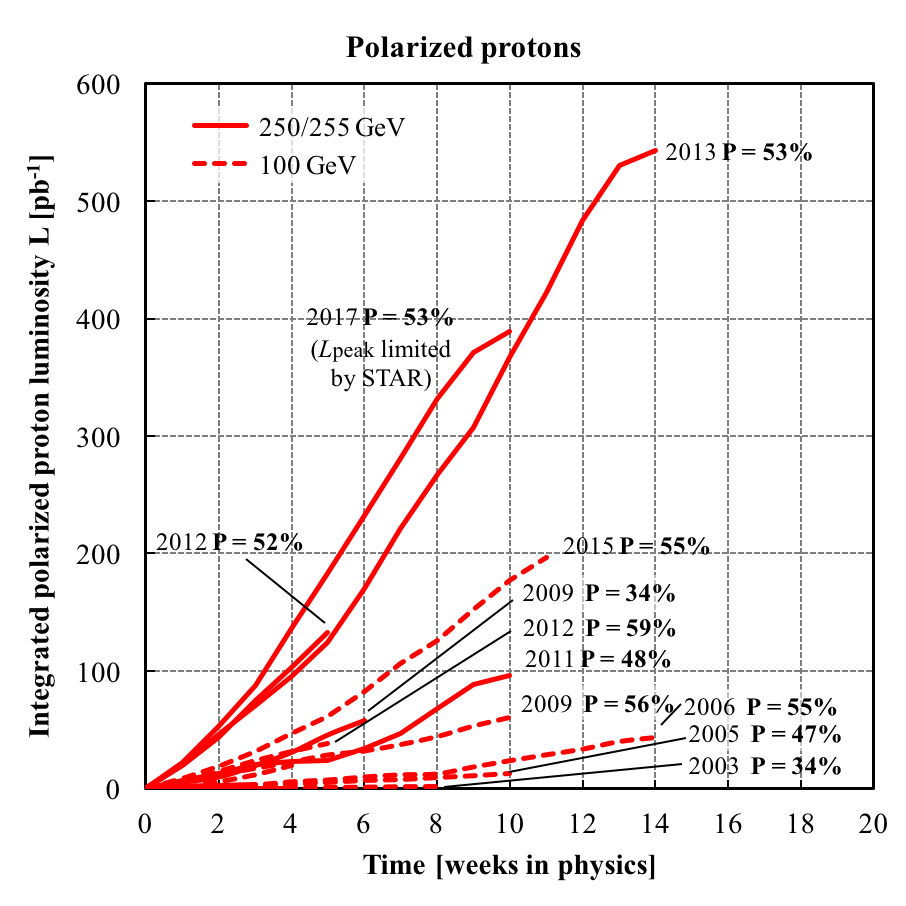
\includegraphics[width=.39\textwidth]{chapters/dataSampleSTAR/img/RhicLuminosityPP.png}
	\hfill
	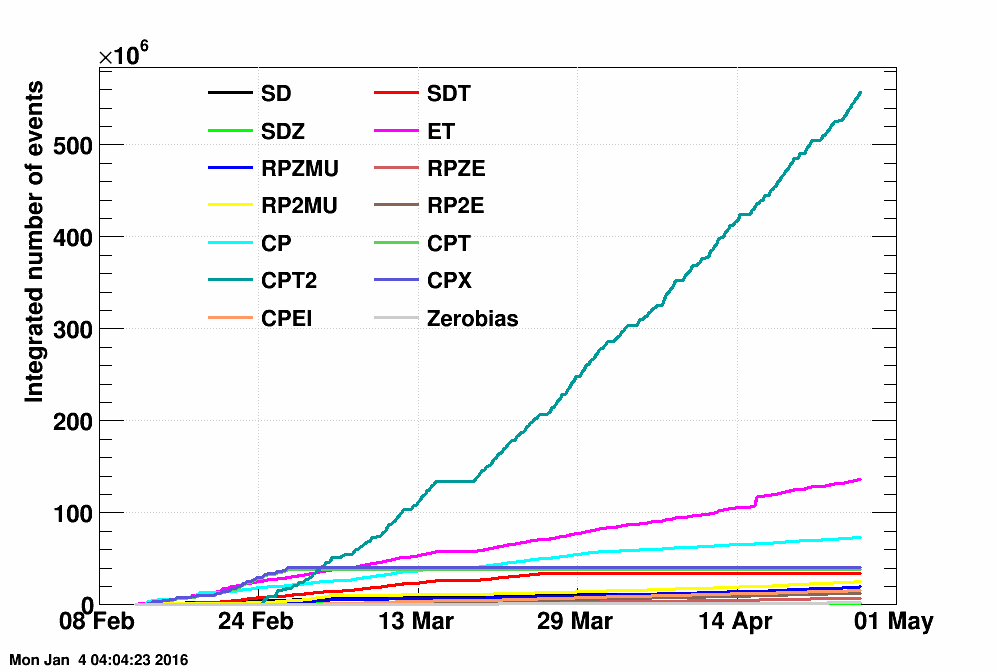
\includegraphics[width=.6\textwidth]{chapters/dataSampleSTAR/img/nEvents.png}
	\caption{(left) Integrated lumonosity delivered by the collider over the seventeen years of operation of RHIC~\cite{RHIC:rhicRunLuminosity}. Dashed lines are for $100$~GeV/c proton momentum mailnly for transverse spin physics programs, while continuous lines are for $250/255$~GeV/c proton beams aimed predominantly at the $W$-physics program. The percentage polarization reached in each run is indicated next to the curves. (right) Integrated number of events collected for each trigger in the~\ac{RP} data stream during Run 15. }
	\label{fig:lumiRHIC}
\end{figure}

All of the studies in this work use data from only the SDT trigger condition, which was the main trigger designed for SDD studies in Run 15 and used in this analysis. It was formed by the following conditions combined with the logical AND:
\begin{enumerate}
	\item RP\_EOR $||$ RP\_WOR - signal in at least one RP on one side of the STAR central detector.
	\item Veto on any signal in small BBC tiles or ZDC on the triggered RP  side of the~STAR central detector.
	\item At least two TOF hits.
\end{enumerate}
Above requirements were imposed in accordance with the diffractive events topology. Veto on any signal in small BBC tiles and ZDC allows to accept only events with rapidity gap and reject diffractive events with parallel pile-up event. The requirement of at least two TOF hits was to ensure activity in the mid-rapidity.

Integrated luminosity delivered by the RHIC to the STAR detector in $pp$ collisions during Run 15 amounts to $185.1$~pb$^{-1}$~\cite{RHIC:rhicRunLuminosity}, shown in Fig.~\ref{fig:lumiRHIC}, whereas about $34.4$M SDT events were gathered by the STAR detector, which corresponds to $16$~nb$^{-1}$ of integrated luminosity.
%\FloatBarrier

%trigger
\section{Online Selection}\label{section:star_trigger_selection}

The first stage of event selection was at online level. The SDT trigger was formed by the following conditions combined with the logical AND:
\begin{enumerate}
	\item RP\_EOR $||$ RP\_WOR - signal in at least one RP on one side of the STAR central detector.
	\item Veto on any signal in small BBC tiles or ZDC on the triggered RP  side of the~STAR central detector.
	\item At least two TOF hits.
\end{enumerate}


Above requirements were imposed in accordance with the diffractive events topology. Veto on any signal in small BBC tiles and ZDC allows to accept only events with rapidity gap and reject diffractive events with parallel pile-up event. The requirement of at least two TOF hits was to ensure activity in the mid-rapidity.
%trigger
\section{Reconstruction}\label{sec:reconstruction}
Raw data was processed with the library version SL17f with the following BFC options:
\vspace{1em}

\noindent\texttt{DbV20160418,pp2015c,btof,mtd,mtdCalib,pp2pp,-beamline,beamline3D, \newline UseBTOFmatchOnly,VFStoreX, fmsDat,fmsPoint,fpsDat,BEmcChkStat,-evout,  \newline CorrX,OSpaceZ2,OGridLeak3D,-hitfilt}
\vspace{1em}

The \texttt{UseBTOFmatchOnly} option was used to form the vertices only from the global TPC tracks matched with TOF hits. It was found that this option provides better signal reconstruction efficiency and resolutions. 

The produced MuDst files (standard STAR data format) were further reduced to Cracow's picoDst data format. 

%nomenclature
%\section{Reconstructed Track Notions}\label{section:star_track_labels}
STAR uses the notions of global and primary tracks. When the event is recorder, the reconstruction algorithm fits a set of TPC hits  with helices, which results in a collection of \textit{global tracks}. Next, all the reconstructed global tracks are extrapolated to the $z$-axis. Tracks that point towards the same vertex are grouped by a minimalization technique and then refitted to include the primary vertex. The resulting tracks are referred to as \textit{primary tracks}, whose momentum resolution is much better in comparison to global tracks.


%event selection
% !TeX spellcheck = en_GB
\subsubsection{Event Selection}\label{section:star_event_selection}
Events were selected from those passing the SDT trigger condition. In order to remove events of poor quality and to suppress background the following conditions were required:
\begin{enumerate}
	\item trigger signals in exactly two stations of one arm of \ac{RP} system (this requirement divides the~sample into four  sub-samples, which were later analysed independently, e.g. for background studies),
	\item any trigger signal in small BBC tiles on the opposite side of the STAR central detector to the~triggered RP station,
	\item exactly one proton track in the above RP stations with $0.02 < \xi < 0.2$ and $0.04 < -t < 0.16$~GeV$^{2}$/c$^{2}$. 
	\item exactly one  vertex  reconstructed from  TPC tracks matched with hits in TOF (later in the~text such vertex  is referred as a TOF vertex),
	\item TOF vertex  within $|V_z|<80$~cm - events with vertices away from the~nominal IP have low acceptance for the central and forward tracks,%~\cite{supplementaryNote},
	\item at least two but no more than eight primary TPC tracks, $2\leq n_{\textrm{sel}}\leq 8$, matched with hits in TOF and satisfying the selection criteria described in Sec.~\ref{section:star_track_selection},
	\item if there are exactly two primary tracks satisfying the~above criteria and exactly two global tracks used in vertex reconstruction (Sec.~\ref{section:star_vertex}), the longitudinal distance between these global tracks should be smaller than $2$~cm, $|\Delta z_0|<2$~cm. %, due to small ($<20\%$) vertex reconstruction efficiency for tracks with $|\Delta z_0|>2$~cm (as described in Sec.~\ref{section:star_vertex}).
\end{enumerate}
Figure~\ref{fig:vertexSTAR} shows the multiplicity of TOF vertices $n_\textrm{vrt}$ (left)  and the $z$-position of  reconstructed vertices in single TOF vertex events (right). Data are compared to embedded PYTHIA~8 SD sample. These distributions are not significantly process-dependent, therefore, contributions from other processes are not included in these plots. Most events with $n_\textrm{vrt} > 1$ originate from in-time pile-up and are excluded from the~analysis.
\begin{figure}[b!]
	\centering
	\includegraphics[width=.49\textwidth, page=13]{chapters/chrgSTAR/img/selection/SDT.pdf}
	\includegraphics[width=.49\textwidth, page=7]{chapters/chrgSTAR/img/selection/SDT.pdf}
	\caption{(left) Vertex multiplicity  and  (right) the~$z$-position of  reconstructed vertices in single TOF vertex events before applying  the~cut on the~quantity shown. Blue lines indicate regions accepted in the analysis.}
	\label{fig:vertexSTAR}
\end{figure}

%\FloatBarrier
%track selection
\section{Track Selection}\label{section:star_track_selection}
The following quality cuts had to be passed by the selected primary tracks in this analysis (TPC and TOF efficiencies are described in~\cite{supplementaryNote}):
\begin{enumerate}
	\item The tracks must be matched with hits reconstructed in TOF,
	\item The number of the  TPC hits used in the helix fit $N_{\textrm{hits}}^{\textrm{fit}}$ must be greater than $24$,
	\item The~ratio of $N_{\textrm{hits}}^{\textrm{fit}}$ to the~number of all possible TPC hits, $N_{\textrm{hits}}^{\textrm{fit}}/N_{\textrm{hits}}^{\textrm{possible}}$, must be greater than $0.52$,
	\item The number of the  TPC hits used to determine the $dE/dx$ information $N_{\textrm{hits}}^{\textrm{dE/dx}}$ must be greater than $14$,
	\item The transverse impact parameter with respect to the beamline $d_0$ must be less than $1.5$~cm,
	\item The radial component of the distance of the closest approach between  the global helix and the vertex $\textrm{DCA}_{xy}$ must be less than $1.5$~cm (consistent with the $d_0$ limit),
	\item The absolute magnitude of  longitudinal component of the distance of the closest approach between  the global helix and the vertex $|\textrm{DCA}_{z}|$ must be less than $1$~cm,
	\item The track's transverse momentum $p_\textrm{T}$ must be greater than $0.2$~GeV/c,
	\item The track's absolute value of  pseudorapidity $|\eta|$ must be smaller than $0.7$.
\end{enumerate}

\begin{figure}[b!]
	\centering
	\begin{subfigure}{.45\textwidth}
		\includegraphics[width=\textwidth, page=10]{chapters/chrgSTAR/img/selection/SDT.pdf}
		\caption{}
	\end{subfigure}
	\begin{subfigure}{.45\textwidth}
		\includegraphics[width=\textwidth, page=9]{chapters/chrgSTAR/img/selection/SDT.pdf}
		\caption{}
	\end{subfigure}
	\begin{subfigure}{.45\textwidth}
		\includegraphics[width=\textwidth, page=5]{chapters/chrgSTAR/img/selection/SDT.pdf}
		\caption{}
	\end{subfigure}
	\begin{subfigure}{.45\textwidth}
		\includegraphics[width=\textwidth, page=6]{chapters/chrgSTAR/img/selection/SDT.pdf}
		\caption{}
	\end{subfigure}
	\begin{subfigure}{.45\textwidth}
		\includegraphics[width=\textwidth, page=11]{chapters/chrgSTAR/img/selection/SDT.pdf}
		\caption{}
	\end{subfigure}
	\begin{minipage}{.45\textwidth}
		
		
		\caption{Number of the  TPC hits used in the helix fit (a) and number of the  TPC hits used to determine the $dE/dx$ (b), the radial component (c) and the absolute magnitude of the longitudinal component (d) of the distance of the closest approach between  the global helix and the vertex, transverse impact parameter w.r.t. beam-line (e). All distributions are shown before applying  the corresponding cuts. Blue lines indicate regions accepted in the analysis.}
		\label{fig:dca_nhitsSTAR}
	\end{minipage}
\end{figure}

\begin{figure}[h!]
	\centering
	\begin{subfigure}{.45\textwidth}
		\includegraphics[width=\textwidth, page=2]{chapters/chrgSTAR/img/selection/SDT.pdf}
		\caption{}
	\end{subfigure}
	\begin{subfigure}{.45\textwidth}
		\includegraphics[width=\textwidth, page=3]{chapters/chrgSTAR/img/selection/SDT.pdf}
		\caption{}
	\end{subfigure}
	\begin{subfigure}{.45\textwidth}
		\includegraphics[width=\textwidth, page=12]{chapters/chrgSTAR/img/selection/SDT_0.pdf}
		\caption{}
	\end{subfigure}
	\begin{subfigure}{.45\textwidth}
		\includegraphics[width=\textwidth, page=12]{chapters/chrgSTAR/img/selection/SDT_1.pdf}
		\caption{}
	\end{subfigure}
	\begin{subfigure}{.45\textwidth}
		\includegraphics[width=\textwidth, page=4]{chapters/chrgSTAR/img/selection/SDT.pdf}
		\caption{}
	\end{subfigure}
	\begin{minipage}{.45\textwidth}
		
		
		\caption{Pseudorapidity of the~reconstructed tracks for events in which forward proton is on  west (a) and east (b) side of the IP, track azimuthal angle for runs $\leq 16073050$ (c) and $>16073050$ (d) and track transverse momentum (e). All distributions are shown before applying  the~corresponding cuts. Blue lines indicate regions accepted in the analysis.}
		\label{fig:ptEtaPhiSTAR}
	\end{minipage}
\end{figure}


The $N_{\textrm{hits}}^{\textrm{fit}}$ and $N_{\textrm{hits}}^{\textrm{fit}}/N_{\textrm{hits}}^{\textrm{possible}}$ cuts are used to reject low quality TPC tracks and avoid track splitting effects. The $d_0$ and global $\textrm{DCA}_{xy}$,  $|\textrm{DCA}_{z}|$ cuts are used to select tracks that originate from the primary interaction vertex. The cut on $N_{\textrm{hits}}^{\textrm{dE/dx}}$ is used to ensure that selected tracks have sufficient energy loss information
for particle identification purposes. In this analysis tracks without identification are required to have $p_\textrm{T} > 0.2$~GeV/c and $|\eta| < 0.7$ due to high track reconstruction and TOF matching efficiencies in this region. For the identified particle-antiparticle ratio analysis, where charged pions, charged kaons and (anti)protons  are measured, the $p_T$ cut was increased for kaons and (anti)protons  to $0.3$ and $0.4$~GeV/c, respectively. 
The distributions of the $\textrm{DCA}_{xy}$, $|\textrm{DCA}_{z}|$, $d_0$, $N_{\textrm{hits}}^{\textrm{fit}}$ and $N_{\textrm{hits}}^{\textrm{dE/dx}}$ quatities together with applied cuts are shown in Fig.~\ref{fig:dca_nhitsSTAR}, while the~$p_T$, $\eta$ and  the~azimuthal angle, $\phi$, of the~reconstructed tracks are shown in Fig.~\ref{fig:ptEtaPhiSTAR}. Data are compared to embedded PYTHIA~8 SD sample. The~azimuthal angle of the~reconstructed tracks for runs $\leq 16073050$ is not described by PYTHIA~8, therefore, additional data-driven corrections to track efficiencies are used~\cite{supplementaryNote}.





%fiducial 
\section{Fiducial Region of the Measurement}\label{section:star_fiducial}
A fiducial phase space of measurement  is defined by the~following criteria. Primary charged particles are defined as charged particles with a mean lifetime $\tau >300$~ps, either directly produced in $pp$ interaction or from subsequent decays of directly produced particles with $\tau <30$~ps. Primary charged particles had to be contained within the kinematic range of $p_\textrm{T}>0.2$~GeV/c and $|\eta|<0.7$.
The~results are corrected to the~region of the total number of primary charged particles (without identification), $2\leq n_\textrm{ch} \leq 8$.  In identified charged antiparticle to particle ratio measurement, the lower transverse momentum limit was set for the analysed particles as follows: $0.2$~GeV/c (pions), $0.3$~GeV/c (kaons), $0.4$~GeV/c (protons and antiprotons).





\begin{figure}[b!]
	\centering
	\includegraphics[width=\textwidth, page=17]{chapters/dataSampleSTAR/img/true.pdf}
	\caption{$\epsilon_{ n_\textrm{ch} \geq 2}$ as a function of $\log_{10}\xi$ calculated from PYTHIA~8 (MBR).}
	\label{fig:STARtrueMCfiducial}
\end{figure}
The measurements were performed in a fiducial phase space of the forward-scattered protons of $0.04<-t<0.16$~GeV$^{2}$/c$^2$ and $0.02 < \xi<0.2$. Figure~\ref{fig:STARtrueMCfiducial} shows that the~fraction  of events containing at least two primary charged particles, $\epsilon_{n_\textrm{ch}\geq 2}(\log_{10}\xi)$,  is reduced by half for $\xi <0.02$ compared to the~region of larger $\xi$. In addition, the~accidental background contribution at $\xi<0.02$  is significant and  approximately equal to $10\%$ (Sec.~\ref{section:star_accidentals}). For these reasons the~lower $\xi$ cut was introduced.  The~upper $\xi$ cut was required since the~region of larger $\xi$ is dominated by \ac{DD} and \ac{ND} (Sec.~\ref{section:star_nonSD}). The joint RP  acceptance and track reconstruction efficiency was defined as the~probability that true-level proton was reconstructed as a~track passing the selection criteria. This efficiency was calculated as a function of $-t$ for three ranges of $\xi$ separately and is shown in Fig.~\ref{fig:STARAcceptance}. 
Events were accepted only if the~reconstructed values of $-t$ for protons fall within $>5\%$ acceptance regions, which were required to be the same for each $\xi$ region  and similar to those defined in the~elastic analysis~\cite{STARelastic2015}. Therefore,  cuts on $0.04 < -t < 0.16$~GeV$^2$/c$^2$ were introduced.
All measured observables are presented in three $\xi$ regions: $0.02<\xi<0.05$, $0.05<\xi<0.1$ and $0.1<\xi<0.2$.
\begin{figure}[h!]
	\thisfloatpagestyle{fancy}
	\centering
	\includegraphics[width=\textwidth, page=4]{chapters/dataSampleSTAR/img/rpeffi.pdf}
	\caption{RP acceptance and track reconstruction efficiency as a~function $-t$ in three ranges of $\xi$, calculated using PYTHIA~8 4C (SaS). Magenta lines indicate region accepted in the~analysis.}
	\label{fig:STARAcceptance}
\end{figure}

\FloatBarrier

%MC sample
\chapter{Monte Carlo Samples }\label{section:star_mc}
\ac{MC} samples used to correct data for detector effects were obtained by the embedding \ac{MC} technique~\cite{STAR:tpc}, in which  simulated particles are mixed with the real Zerobias events at the raw data level. Zerobias data events used in the embedding were sampled over the entire data-taking period in order to properly describe the data set used in the analysis.  Two samples of embedding MC were produced:
\begin{enumerate}
	\item Single particle \ac{MC}, in which particles are generated from flat distributions in $\eta$ and $p_\textrm{T}$, in order to have similar statistics in all bins.
	\item The \ac{SaS} model implemented in PYTHIA~8 with 4C tune. 
\end{enumerate}
The particles were propagated through the full simulation of the STAR TPC and RP system detectors using GEANT3~\cite{GEANT:three} and GEANT4~\cite{GEANT:four}, respectively. Obtained information for the simulated particles was embedded into the existing information of the real data. These events were next processed through the~full reconstruction chain. 

An~iterative unfolding procedure was used to express the track multiplicity in terms of the~number of charged particles.  The~unfolding matrices were obtained from PYTHIA~8 4C (\ac{SaS}). In order to keep statistical precision coming
from the~matrices high, samples filtered on true-level values of $\xi$ and $t$ (not necessarily with reconstructed proton track in RP) are used. 

It is preferred to get the detector corrections from a~MC, which is dedicated to simulate the~studied  physics process. However, for this purpose, the statistics in the MC should be several times greater than we have in the data for analysis. Since this is not possible with  low efficiency of TPC and TOF, the basic method of corrections used in the analysis for $p_\textrm{T}$ and $\bar{\eta}$ distributions is a~method of factorization of global efficiency into the product of single-particle efficiencies. In this way, statistically precise multidimensional corrections on TPC and TOF were obtained from the~single particle MC. %These corrections were not applied to charged-particle multiplicity distributions since  the~unfolding matrices already contain TPC and TOF efficiencies.
The~charged-particle multiplicity distributions were unfolded from the~measured multiplicities of TPC tracks based on the~response matrix, which takes into account  all detector effects and was obtained from PYTHIA 8 4C (SaS) simulation of SD process. In this procedure single particle MC samples were not used.  



%For charged-particle multiplicity distributions 
 %Dla n_ch  robi Pan unfolding i korzysta z PYTHII.
 %To trzeba napisać.  Ale nadal  jak rozumiem faktoryzuje Pan stan centralny i protony do przodu w tym sensie, że macierze odpowiedzi maja cięcie na 
 %xi i t na poziomie true, bez wymagania obserwacji protonu w RP.

Several additional MC samples were generated, in which  simulated particles were propagated through full simulation and reconstruction chain but were  not embedded  into Zerobias events.   
Systematic effect related to hadronization of the diffractive system was determined by using alternative hadronization models implemented in HERWIG and EPOS. Results are compared to model predictions from PYTHIA 8 4C (\ac{SaS}), HERWIG, EPOS and alternative PYTHIA 8 model  \ac{MBR}  with A2 tune. EPOS predicts very large contribution of forward 
protons, which originate from non-diffractive events and are well separated in rapidity from other final state particles. This is the result of low mass excitation of the proton remnant ($<1$ GeV) leading to hadronization of the beam remnant back to the proton. Therefore EPOS predictions were separated in two classes: diffractive (EPOS SD) modelled by Pomeron exchange and non-diffractive modelled  by low mass excitation of the proton remnant (EPOS SD$^\prime$). Such remnant treatment is very unique in EPOS compared to other string models, especially, to that used in PYTHIA~8, where \ac{ND} forward protons are rare 
and  arise from string fragmentation and hadronization. In all PYTHIA~8 models, diffractive cross-sections are scaled by the~fudge factors, which were introduced in order to describe the~full phase space~\cite{Sjostrand:2006za,MBR:intro}. In the~\ac{SaS} model, the~fudge factors for SD and DD,  $F_{\textrm{SD}}$ and $F_{\textrm{DD}}$, are defined as a~function of diffractive masses:

\begin{equation}
F_{\textrm{SD}}=\left(1-\frac{M^2}{s}\right)\left(1+\frac{c_\textrm{res}M^2_\textrm{res}}{M^2_\textrm{res}+M^2}\right)
\end{equation}

\begin{equation}
F_{\textrm{DD}}=\left(1-\frac{M_a^2+M_b^2}{s}\right)\left(\frac{sm^2_p}{sm^2_p+M_a^2M_b^2}\right)\times
\left(1+\frac{c_\textrm{res}M_\textrm{res}^2}{M_\textrm{res}^2+M_a^2}\right)\left(1+\frac{c_\textrm{res}M_\textrm{res}^2}{M_\textrm{res}^2+M_b^2}\right)
\end{equation}
where $M$ and $M_{a}$, $M_{b}$ are the~invariant masses of the~systems $X$ and $X_a$, $X_b$ for SD and DD, respectively, $c_\textrm{res}=2$ and $M_\textrm{res}=2$~GeV/c$^2$ were obtained from a~fit to $pp/\bar{p}p$ data~\cite{Sjostrand:2006za}. On the~other hand, in the~\ac{MBR} model the~fudge factor is given as a function of the~rapidity gap~\cite{MBR:intro}:
\begin{equation}
S=\frac{1}{2}\left[1+\textrm{erf}\left(\frac{\Delta y-\Delta y_S}{\sigma_S}\right)\right]
\end{equation}
where $\Delta y$ is the~rapidity gap, $\Delta y_S=2$ and $\sigma_S=0.5$. As a result, diffractive cross sections are artificially suppressed at 
relatively large values of $\xi$ ($>$0.05). This artificial suppression significantly changes predicted distribution of $\xi$ and fractions of different processes in our fiducial phase space. Therefore data is also compared with expectations obtained without suppression of the~diffractive cross sections (MBR-tuned).

Figure~\ref{fig:STARtrueMC} shows $\xi$ and $|t|$ distributions generated with  EPOS (SD and SD+SD$^\prime$) and PYTHIA~8 SD (MBR and MBR-tuned). There are differences among models in both the~low and high $\xi$ regions. The~minimum value of $|t|$ depends on the mass of the~diffractive system, hence, all models predict suppression of the~cross-section at small $|t|$. EPOS SD is only relevant for very small $|t|$ and is suppressed in the~STAR acceptance region, $0.04<|t|<0.16$, where EPOS SD$^\prime$ contribution dominates. In addition, the $t$-slope is  very different for EPOS SD and SD$^\prime$, while it is similar for EPOS SD$^\prime$ and PYTHIA~8 predictions. The~PYTHIA~8 (MBR-tuned) expectations, as opposed to the~MBR model,  lead
to the~larger cross-sections in the high-mass regions.
 
\begin{figure}[h!]
	\centering
	\includegraphics[width=0.49\textwidth, page=14]{chapters/dataSampleSTAR/img/true.pdf}
	\includegraphics[width=0.49\textwidth, page=13]{chapters/dataSampleSTAR/img/true.pdf}
	\caption{(left) $\xi$ and  (right) $|t|$ distributions for various MC generators at $\sqrt{s} = 200$~GeV.}
	\label{fig:STARtrueMC}
\end{figure}

%Analysis STAR
%\chapter{STAR Data Analysis}\label{chapter:star_analysis}
%\section{Roman Pot Simulation}\label{section:reconstructionSTAR_pp2pp_Sim}
\begin{figure}[h!]
	\centering
	\begin{subfigure}{.64\textwidth}
		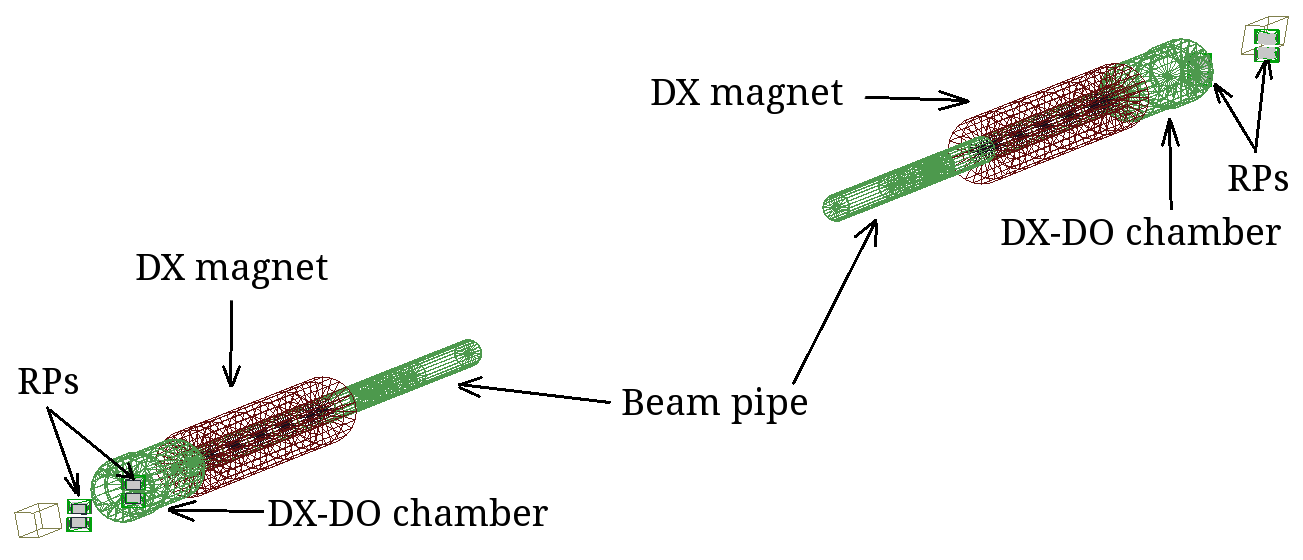
\includegraphics[width=\textwidth]{chapters/dataSampleSTAR/img/pp2ppSim/geant4plot.png}
	\end{subfigure}
	\begin{subfigure}{.34\textwidth}
		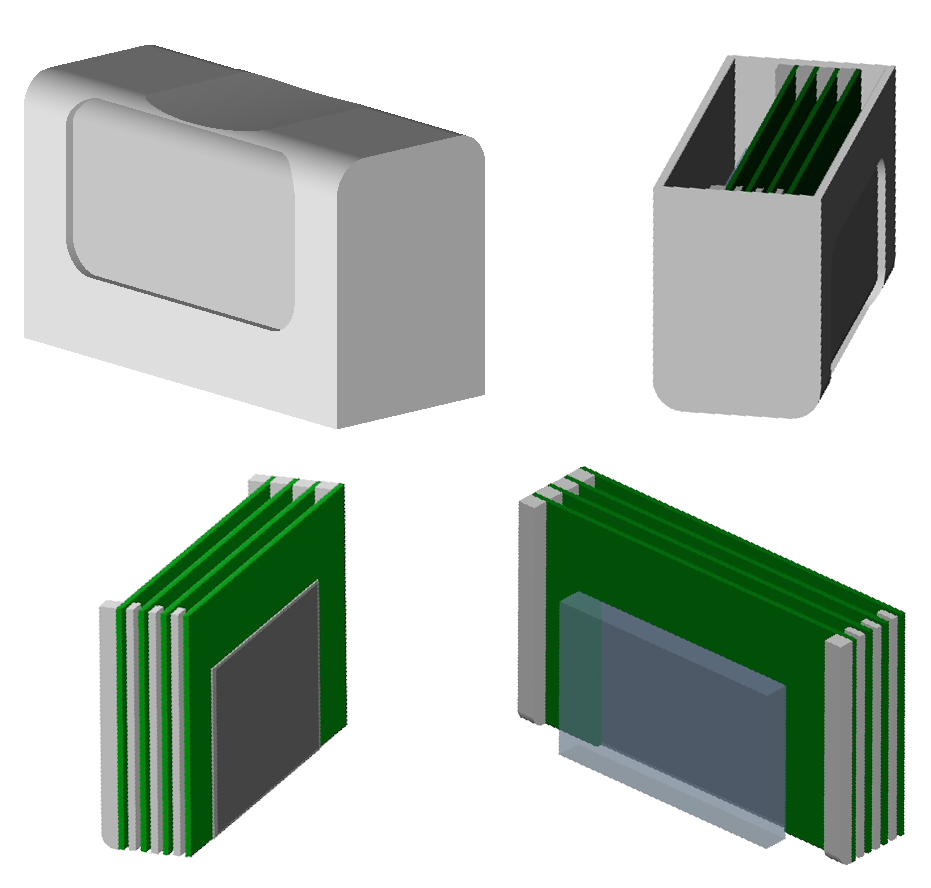
\includegraphics[width=\textwidth]{chapters/dataSampleSTAR/img/pp2ppSim/g4Rp.png}
	\end{subfigure}	
	
	\caption{(left) GEANT4 implementation of the RP system and (right) RP vessel together with SSD. Figure courtesy of R. Sikora (STAR Collaboration).}
	\label{fig:pp2ppSim}
\end{figure}

The geometry of the \ac{RP} detectors is not implemented in the~standard \ac{STAR} GEANT3 simulation. Therefore, a~standalone GEANT4 simulation of the \ac{RP} \ac{SSD} detectors~\cite{RafalInz,RafalMgr} and the \ac{RHIC} magnet lattice was developed~\cite{LukaszInz,LukaszMgr}. The application was orginally dedicated to the configuration of the \ac{RP}s for RHIC Run 2009~\cite{pp2pp:elastic}. When the \ac{RP}s were moved to their current location in the \ac{RHIC} tunnel, the simulation was updated. The geometry of  \ac{RHIC}, i.e. magnets and beampipe, is based on the technical drawings of  \ac{RHIC}, whereas the MAD-X~\cite{MADX} output provides information about the magnetic field of the RHIC DX magnets. In case of the \ac{RP} vessels and \ac{SSD}s, technical drawings together with the dedicated survey were used to best implement their geometry.

Figure~\ref{fig:pp2ppSim} shows the GEANT4 visualisation of the \ac{RP} setup together with all beam-line elements. In addition, the  implementation of the \ac{RP} vessels and \ac{SSD}s is  presented. 



 

%MC sample
\chapter{Monte Carlo Samples }\label{section:star_mc}
\ac{MC} samples used to correct data for detector effects were obtained by the embedding \ac{MC} technique~\cite{STAR:tpc}, in which  simulated particles are mixed with the real Zerobias events at the raw data level. Zerobias data events used in the embedding were sampled over the entire data-taking period in order to properly describe the data set used in the analysis.  Two samples of embedding MC were produced:
\begin{enumerate}
	\item Single particle \ac{MC}, in which particles are generated from flat distributions in $\eta$ and $p_\textrm{T}$, in order to have similar statistics in all bins.
	\item The \ac{SaS} model implemented in PYTHIA~8 with 4C tune. 
\end{enumerate}
The particles were propagated through the full simulation of the STAR TPC and RP system detectors using GEANT3~\cite{GEANT:three} and GEANT4~\cite{GEANT:four}, respectively. Obtained information for the simulated particles was embedded into the existing information of the real data. These events were next processed through the~full reconstruction chain. 

An~iterative unfolding procedure was used to express the track multiplicity in terms of the~number of charged particles.  The~unfolding matrices were obtained from PYTHIA~8 4C (\ac{SaS}). In order to keep statistical precision coming
from the~matrices high, samples filtered on true-level values of $\xi$ and $t$ (not necessarily with reconstructed proton track in RP) are used. 

It is preferred to get the detector corrections from a~MC, which is dedicated to simulate the~studied  physics process. However, for this purpose, the statistics in the MC should be several times greater than we have in the data for analysis. Since this is not possible with  low efficiency of TPC and TOF, the basic method of corrections used in the analysis for $p_\textrm{T}$ and $\bar{\eta}$ distributions is a~method of factorization of global efficiency into the product of single-particle efficiencies. In this way, statistically precise multidimensional corrections on TPC and TOF were obtained from the~single particle MC. %These corrections were not applied to charged-particle multiplicity distributions since  the~unfolding matrices already contain TPC and TOF efficiencies.
The~charged-particle multiplicity distributions were unfolded from the~measured multiplicities of TPC tracks based on the~response matrix, which takes into account  all detector effects and was obtained from PYTHIA 8 4C (SaS) simulation of SD process. In this procedure single particle MC samples were not used.  



%For charged-particle multiplicity distributions 
 %Dla n_ch  robi Pan unfolding i korzysta z PYTHII.
 %To trzeba napisać.  Ale nadal  jak rozumiem faktoryzuje Pan stan centralny i protony do przodu w tym sensie, że macierze odpowiedzi maja cięcie na 
 %xi i t na poziomie true, bez wymagania obserwacji protonu w RP.

Several additional MC samples were generated, in which  simulated particles were propagated through full simulation and reconstruction chain but were  not embedded  into Zerobias events.   
Systematic effect related to hadronization of the diffractive system was determined by using alternative hadronization models implemented in HERWIG and EPOS. Results are compared to model predictions from PYTHIA 8 4C (\ac{SaS}), HERWIG, EPOS and alternative PYTHIA 8 model  \ac{MBR}  with A2 tune. EPOS predicts very large contribution of forward 
protons, which originate from non-diffractive events and are well separated in rapidity from other final state particles. This is the result of low mass excitation of the proton remnant ($<1$ GeV) leading to hadronization of the beam remnant back to the proton. Therefore EPOS predictions were separated in two classes: diffractive (EPOS SD) modelled by Pomeron exchange and non-diffractive modelled  by low mass excitation of the proton remnant (EPOS SD$^\prime$). Such remnant treatment is very unique in EPOS compared to other string models, especially, to that used in PYTHIA~8, where \ac{ND} forward protons are rare 
and  arise from string fragmentation and hadronization. In all PYTHIA~8 models, diffractive cross-sections are scaled by the~fudge factors, which were introduced in order to describe the~full phase space~\cite{Sjostrand:2006za,MBR:intro}. In the~\ac{SaS} model, the~fudge factors for SD and DD,  $F_{\textrm{SD}}$ and $F_{\textrm{DD}}$, are defined as a~function of diffractive masses:

\begin{equation}
F_{\textrm{SD}}=\left(1-\frac{M^2}{s}\right)\left(1+\frac{c_\textrm{res}M^2_\textrm{res}}{M^2_\textrm{res}+M^2}\right)
\end{equation}

\begin{equation}
F_{\textrm{DD}}=\left(1-\frac{M_a^2+M_b^2}{s}\right)\left(\frac{sm^2_p}{sm^2_p+M_a^2M_b^2}\right)\times
\left(1+\frac{c_\textrm{res}M_\textrm{res}^2}{M_\textrm{res}^2+M_a^2}\right)\left(1+\frac{c_\textrm{res}M_\textrm{res}^2}{M_\textrm{res}^2+M_b^2}\right)
\end{equation}
where $M$ and $M_{a}$, $M_{b}$ are the~invariant masses of the~systems $X$ and $X_a$, $X_b$ for SD and DD, respectively, $c_\textrm{res}=2$ and $M_\textrm{res}=2$~GeV/c$^2$ were obtained from a~fit to $pp/\bar{p}p$ data~\cite{Sjostrand:2006za}. On the~other hand, in the~\ac{MBR} model the~fudge factor is given as a function of the~rapidity gap~\cite{MBR:intro}:
\begin{equation}
S=\frac{1}{2}\left[1+\textrm{erf}\left(\frac{\Delta y-\Delta y_S}{\sigma_S}\right)\right]
\end{equation}
where $\Delta y$ is the~rapidity gap, $\Delta y_S=2$ and $\sigma_S=0.5$. As a result, diffractive cross sections are artificially suppressed at 
relatively large values of $\xi$ ($>$0.05). This artificial suppression significantly changes predicted distribution of $\xi$ and fractions of different processes in our fiducial phase space. Therefore data is also compared with expectations obtained without suppression of the~diffractive cross sections (MBR-tuned).

Figure~\ref{fig:STARtrueMC} shows $\xi$ and $|t|$ distributions generated with  EPOS (SD and SD+SD$^\prime$) and PYTHIA~8 SD (MBR and MBR-tuned). There are differences among models in both the~low and high $\xi$ regions. The~minimum value of $|t|$ depends on the mass of the~diffractive system, hence, all models predict suppression of the~cross-section at small $|t|$. EPOS SD is only relevant for very small $|t|$ and is suppressed in the~STAR acceptance region, $0.04<|t|<0.16$, where EPOS SD$^\prime$ contribution dominates. In addition, the $t$-slope is  very different for EPOS SD and SD$^\prime$, while it is similar for EPOS SD$^\prime$ and PYTHIA~8 predictions. The~PYTHIA~8 (MBR-tuned) expectations, as opposed to the~MBR model,  lead
to the~larger cross-sections in the high-mass regions.
 
\begin{figure}[h!]
	\centering
	\includegraphics[width=0.49\textwidth, page=14]{chapters/dataSampleSTAR/img/true.pdf}
	\includegraphics[width=0.49\textwidth, page=13]{chapters/dataSampleSTAR/img/true.pdf}
	\caption{(left) $\xi$ and  (right) $|t|$ distributions for various MC generators at $\sqrt{s} = 200$~GeV.}
	\label{fig:STARtrueMC}
\end{figure}

%data sample
\chapter{Data Sample and Signal Selection}\label{section:star_data_sample}\label{section:star_trigger_selection}
The data sample used in this analysis was collected in proton-proton collisions at centre-of-mass energy of $\sqrt{s}=200$~GeV during RHIC Run 15, i.e. in year 2015. %Data from the RP related triggers is stored in a~special data stream.  

\begin{figure}[h!]
	\centering
	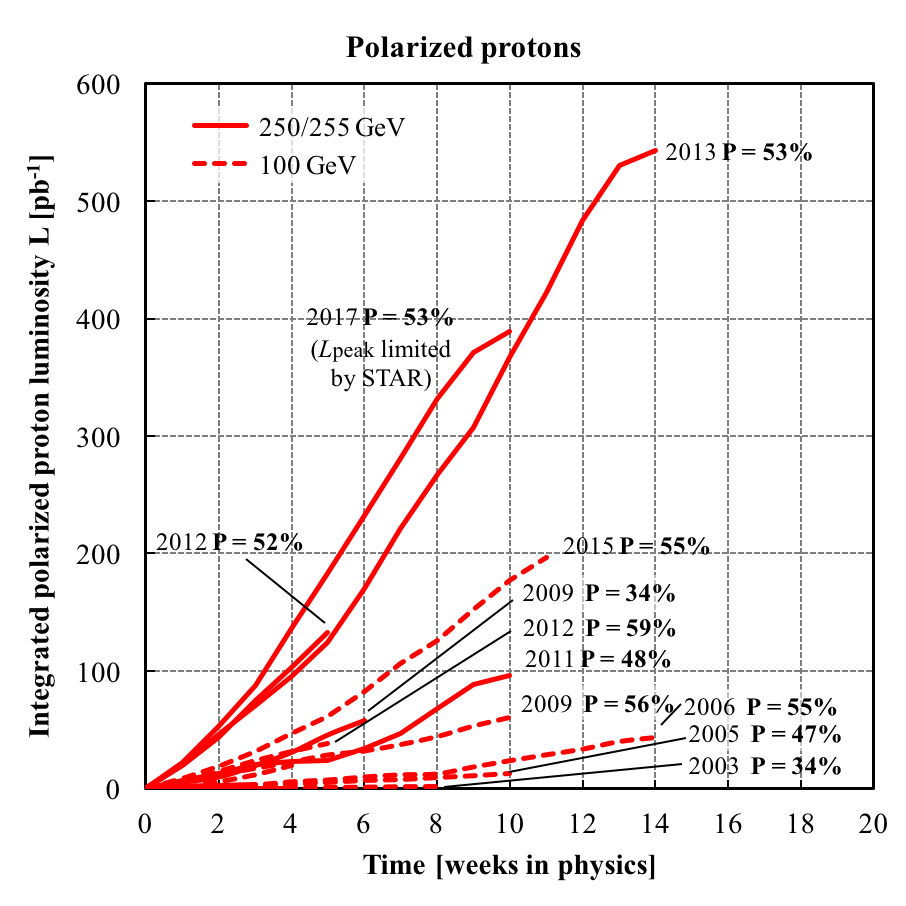
\includegraphics[width=.39\textwidth]{chapters/dataSampleSTAR/img/RhicLuminosityPP.png}
	\hfill
	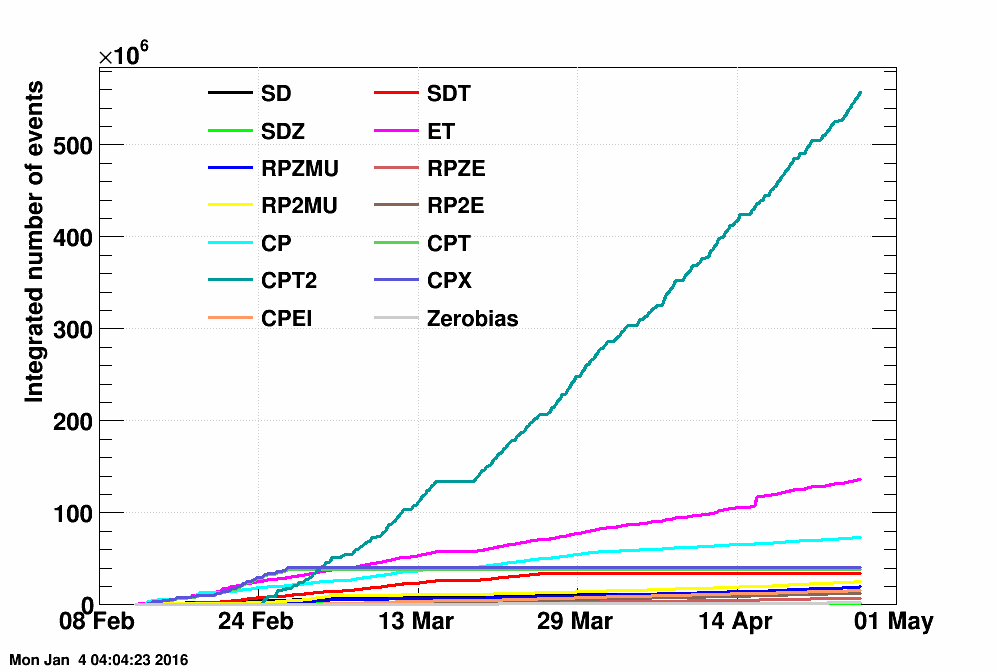
\includegraphics[width=.6\textwidth]{chapters/dataSampleSTAR/img/nEvents.png}
	\caption{(left) Integrated lumonosity delivered by the collider over the seventeen years of operation of RHIC~\cite{RHIC:rhicRunLuminosity}. Dashed lines are for $100$~GeV/c proton momentum mailnly for transverse spin physics programs, while continuous lines are for $250/255$~GeV/c proton beams aimed predominantly at the $W$-physics program. The percentage polarization reached in each run is indicated next to the curves. (right) Integrated number of events collected for each trigger in the~\ac{RP} data stream during Run 15. }
	\label{fig:lumiRHIC}
\end{figure}

All of the studies in this work use data from only the SDT trigger condition, which was the main trigger designed for SDD studies in Run 15 and used in this analysis. It was formed by the following conditions combined with the logical AND:
\begin{enumerate}
	\item RP\_EOR $||$ RP\_WOR - signal in at least one RP on one side of the STAR central detector.
	\item Veto on any signal in small BBC tiles or ZDC on the triggered RP  side of the~STAR central detector.
	\item At least two TOF hits.
\end{enumerate}
Above requirements were imposed in accordance with the diffractive events topology. Veto on any signal in small BBC tiles and ZDC allows to accept only events with rapidity gap and reject diffractive events with parallel pile-up event. The requirement of at least two TOF hits was to ensure activity in the mid-rapidity.

Integrated luminosity delivered by the RHIC to the STAR detector in $pp$ collisions during Run 15 amounts to $185.1$~pb$^{-1}$~\cite{RHIC:rhicRunLuminosity}, shown in Fig.~\ref{fig:lumiRHIC}, whereas about $34.4$M SDT events were gathered by the STAR detector, which corresponds to $16$~nb$^{-1}$ of integrated luminosity.
%\FloatBarrier

%trigger
%\section{Online Selection}\label{section:star_trigger_selection}

The first stage of event selection was at online level. The SDT trigger was formed by the following conditions combined with the logical AND:
\begin{enumerate}
	\item RP\_EOR $||$ RP\_WOR - signal in at least one RP on one side of the STAR central detector.
	\item Veto on any signal in small BBC tiles or ZDC on the triggered RP  side of the~STAR central detector.
	\item At least two TOF hits.
\end{enumerate}


Above requirements were imposed in accordance with the diffractive events topology. Veto on any signal in small BBC tiles and ZDC allows to accept only events with rapidity gap and reject diffractive events with parallel pile-up event. The requirement of at least two TOF hits was to ensure activity in the mid-rapidity.%poszlo do dataSample

%event selection
% !TeX spellcheck = en_GB
\subsubsection{Event Selection}\label{section:star_event_selection}
Events were selected from those passing the SDT trigger condition. In order to remove events of poor quality and to suppress background the following conditions were required:
\begin{enumerate}
	\item trigger signals in exactly two stations of one arm of \ac{RP} system (this requirement divides the~sample into four  sub-samples, which were later analysed independently, e.g. for background studies),
	\item any trigger signal in small BBC tiles on the opposite side of the STAR central detector to the~triggered RP station,
	\item exactly one proton track in the above RP stations with $0.02 < \xi < 0.2$ and $0.04 < -t < 0.16$~GeV$^{2}$/c$^{2}$. 
	\item exactly one  vertex  reconstructed from  TPC tracks matched with hits in TOF (later in the~text such vertex  is referred as a TOF vertex),
	\item TOF vertex  within $|V_z|<80$~cm - events with vertices away from the~nominal IP have low acceptance for the central and forward tracks,%~\cite{supplementaryNote},
	\item at least two but no more than eight primary TPC tracks, $2\leq n_{\textrm{sel}}\leq 8$, matched with hits in TOF and satisfying the selection criteria described in Sec.~\ref{section:star_track_selection},
	\item if there are exactly two primary tracks satisfying the~above criteria and exactly two global tracks used in vertex reconstruction (Sec.~\ref{section:star_vertex}), the longitudinal distance between these global tracks should be smaller than $2$~cm, $|\Delta z_0|<2$~cm. %, due to small ($<20\%$) vertex reconstruction efficiency for tracks with $|\Delta z_0|>2$~cm (as described in Sec.~\ref{section:star_vertex}).
\end{enumerate}
Figure~\ref{fig:vertexSTAR} shows the multiplicity of TOF vertices $n_\textrm{vrt}$ (left)  and the $z$-position of  reconstructed vertices in single TOF vertex events (right). Data are compared to embedded PYTHIA~8 SD sample. These distributions are not significantly process-dependent, therefore, contributions from other processes are not included in these plots. Most events with $n_\textrm{vrt} > 1$ originate from in-time pile-up and are excluded from the~analysis.
\begin{figure}[b!]
	\centering
	\includegraphics[width=.49\textwidth, page=13]{chapters/chrgSTAR/img/selection/SDT.pdf}
	\includegraphics[width=.49\textwidth, page=7]{chapters/chrgSTAR/img/selection/SDT.pdf}
	\caption{(left) Vertex multiplicity  and  (right) the~$z$-position of  reconstructed vertices in single TOF vertex events before applying  the~cut on the~quantity shown. Blue lines indicate regions accepted in the analysis.}
	\label{fig:vertexSTAR}
\end{figure}

%\FloatBarrier
%track selection
\section{Track Selection}\label{section:star_track_selection}
The following quality cuts had to be passed by the selected primary tracks in this analysis (TPC and TOF efficiencies are described in~\cite{supplementaryNote}):
\begin{enumerate}
	\item The tracks must be matched with hits reconstructed in TOF,
	\item The number of the  TPC hits used in the helix fit $N_{\textrm{hits}}^{\textrm{fit}}$ must be greater than $24$,
	\item The~ratio of $N_{\textrm{hits}}^{\textrm{fit}}$ to the~number of all possible TPC hits, $N_{\textrm{hits}}^{\textrm{fit}}/N_{\textrm{hits}}^{\textrm{possible}}$, must be greater than $0.52$,
	\item The number of the  TPC hits used to determine the $dE/dx$ information $N_{\textrm{hits}}^{\textrm{dE/dx}}$ must be greater than $14$,
	\item The transverse impact parameter with respect to the beamline $d_0$ must be less than $1.5$~cm,
	\item The radial component of the distance of the closest approach between  the global helix and the vertex $\textrm{DCA}_{xy}$ must be less than $1.5$~cm (consistent with the $d_0$ limit),
	\item The absolute magnitude of  longitudinal component of the distance of the closest approach between  the global helix and the vertex $|\textrm{DCA}_{z}|$ must be less than $1$~cm,
	\item The track's transverse momentum $p_\textrm{T}$ must be greater than $0.2$~GeV/c,
	\item The track's absolute value of  pseudorapidity $|\eta|$ must be smaller than $0.7$.
\end{enumerate}

\begin{figure}[b!]
	\centering
	\begin{subfigure}{.45\textwidth}
		\includegraphics[width=\textwidth, page=10]{chapters/chrgSTAR/img/selection/SDT.pdf}
		\caption{}
	\end{subfigure}
	\begin{subfigure}{.45\textwidth}
		\includegraphics[width=\textwidth, page=9]{chapters/chrgSTAR/img/selection/SDT.pdf}
		\caption{}
	\end{subfigure}
	\begin{subfigure}{.45\textwidth}
		\includegraphics[width=\textwidth, page=5]{chapters/chrgSTAR/img/selection/SDT.pdf}
		\caption{}
	\end{subfigure}
	\begin{subfigure}{.45\textwidth}
		\includegraphics[width=\textwidth, page=6]{chapters/chrgSTAR/img/selection/SDT.pdf}
		\caption{}
	\end{subfigure}
	\begin{subfigure}{.45\textwidth}
		\includegraphics[width=\textwidth, page=11]{chapters/chrgSTAR/img/selection/SDT.pdf}
		\caption{}
	\end{subfigure}
	\begin{minipage}{.45\textwidth}
		
		
		\caption{Number of the  TPC hits used in the helix fit (a) and number of the  TPC hits used to determine the $dE/dx$ (b), the radial component (c) and the absolute magnitude of the longitudinal component (d) of the distance of the closest approach between  the global helix and the vertex, transverse impact parameter w.r.t. beam-line (e). All distributions are shown before applying  the corresponding cuts. Blue lines indicate regions accepted in the analysis.}
		\label{fig:dca_nhitsSTAR}
	\end{minipage}
\end{figure}

\begin{figure}[h!]
	\centering
	\begin{subfigure}{.45\textwidth}
		\includegraphics[width=\textwidth, page=2]{chapters/chrgSTAR/img/selection/SDT.pdf}
		\caption{}
	\end{subfigure}
	\begin{subfigure}{.45\textwidth}
		\includegraphics[width=\textwidth, page=3]{chapters/chrgSTAR/img/selection/SDT.pdf}
		\caption{}
	\end{subfigure}
	\begin{subfigure}{.45\textwidth}
		\includegraphics[width=\textwidth, page=12]{chapters/chrgSTAR/img/selection/SDT_0.pdf}
		\caption{}
	\end{subfigure}
	\begin{subfigure}{.45\textwidth}
		\includegraphics[width=\textwidth, page=12]{chapters/chrgSTAR/img/selection/SDT_1.pdf}
		\caption{}
	\end{subfigure}
	\begin{subfigure}{.45\textwidth}
		\includegraphics[width=\textwidth, page=4]{chapters/chrgSTAR/img/selection/SDT.pdf}
		\caption{}
	\end{subfigure}
	\begin{minipage}{.45\textwidth}
		
		
		\caption{Pseudorapidity of the~reconstructed tracks for events in which forward proton is on  west (a) and east (b) side of the IP, track azimuthal angle for runs $\leq 16073050$ (c) and $>16073050$ (d) and track transverse momentum (e). All distributions are shown before applying  the~corresponding cuts. Blue lines indicate regions accepted in the analysis.}
		\label{fig:ptEtaPhiSTAR}
	\end{minipage}
\end{figure}


The $N_{\textrm{hits}}^{\textrm{fit}}$ and $N_{\textrm{hits}}^{\textrm{fit}}/N_{\textrm{hits}}^{\textrm{possible}}$ cuts are used to reject low quality TPC tracks and avoid track splitting effects. The $d_0$ and global $\textrm{DCA}_{xy}$,  $|\textrm{DCA}_{z}|$ cuts are used to select tracks that originate from the primary interaction vertex. The cut on $N_{\textrm{hits}}^{\textrm{dE/dx}}$ is used to ensure that selected tracks have sufficient energy loss information
for particle identification purposes. In this analysis tracks without identification are required to have $p_\textrm{T} > 0.2$~GeV/c and $|\eta| < 0.7$ due to high track reconstruction and TOF matching efficiencies in this region. For the identified particle-antiparticle ratio analysis, where charged pions, charged kaons and (anti)protons  are measured, the $p_T$ cut was increased for kaons and (anti)protons  to $0.3$ and $0.4$~GeV/c, respectively. 
The distributions of the $\textrm{DCA}_{xy}$, $|\textrm{DCA}_{z}|$, $d_0$, $N_{\textrm{hits}}^{\textrm{fit}}$ and $N_{\textrm{hits}}^{\textrm{dE/dx}}$ quatities together with applied cuts are shown in Fig.~\ref{fig:dca_nhitsSTAR}, while the~$p_T$, $\eta$ and  the~azimuthal angle, $\phi$, of the~reconstructed tracks are shown in Fig.~\ref{fig:ptEtaPhiSTAR}. Data are compared to embedded PYTHIA~8 SD sample. The~azimuthal angle of the~reconstructed tracks for runs $\leq 16073050$ is not described by PYTHIA~8, therefore, additional data-driven corrections to track efficiencies are used~\cite{supplementaryNote}.





%fiducial 
\section{Fiducial Region of the Measurement}\label{section:star_fiducial}
A fiducial phase space of measurement  is defined by the~following criteria. Primary charged particles are defined as charged particles with a mean lifetime $\tau >300$~ps, either directly produced in $pp$ interaction or from subsequent decays of directly produced particles with $\tau <30$~ps. Primary charged particles had to be contained within the kinematic range of $p_\textrm{T}>0.2$~GeV/c and $|\eta|<0.7$.
The~results are corrected to the~region of the total number of primary charged particles (without identification), $2\leq n_\textrm{ch} \leq 8$.  In identified charged antiparticle to particle ratio measurement, the lower transverse momentum limit was set for the analysed particles as follows: $0.2$~GeV/c (pions), $0.3$~GeV/c (kaons), $0.4$~GeV/c (protons and antiprotons).





\begin{figure}[b!]
	\centering
	\includegraphics[width=\textwidth, page=17]{chapters/dataSampleSTAR/img/true.pdf}
	\caption{$\epsilon_{ n_\textrm{ch} \geq 2}$ as a function of $\log_{10}\xi$ calculated from PYTHIA~8 (MBR).}
	\label{fig:STARtrueMCfiducial}
\end{figure}
The measurements were performed in a fiducial phase space of the forward-scattered protons of $0.04<-t<0.16$~GeV$^{2}$/c$^2$ and $0.02 < \xi<0.2$. Figure~\ref{fig:STARtrueMCfiducial} shows that the~fraction  of events containing at least two primary charged particles, $\epsilon_{n_\textrm{ch}\geq 2}(\log_{10}\xi)$,  is reduced by half for $\xi <0.02$ compared to the~region of larger $\xi$. In addition, the~accidental background contribution at $\xi<0.02$  is significant and  approximately equal to $10\%$ (Sec.~\ref{section:star_accidentals}). For these reasons the~lower $\xi$ cut was introduced.  The~upper $\xi$ cut was required since the~region of larger $\xi$ is dominated by \ac{DD} and \ac{ND} (Sec.~\ref{section:star_nonSD}). The joint RP  acceptance and track reconstruction efficiency was defined as the~probability that true-level proton was reconstructed as a~track passing the selection criteria. This efficiency was calculated as a function of $-t$ for three ranges of $\xi$ separately and is shown in Fig.~\ref{fig:STARAcceptance}. 
Events were accepted only if the~reconstructed values of $-t$ for protons fall within $>5\%$ acceptance regions, which were required to be the same for each $\xi$ region  and similar to those defined in the~elastic analysis~\cite{STARelastic2015}. Therefore,  cuts on $0.04 < -t < 0.16$~GeV$^2$/c$^2$ were introduced.
All measured observables are presented in three $\xi$ regions: $0.02<\xi<0.05$, $0.05<\xi<0.1$ and $0.1<\xi<0.2$.
\begin{figure}[h!]
	\thisfloatpagestyle{fancy}
	\centering
	\includegraphics[width=\textwidth, page=4]{chapters/dataSampleSTAR/img/rpeffi.pdf}
	\caption{RP acceptance and track reconstruction efficiency as a~function $-t$ in three ranges of $\xi$, calculated using PYTHIA~8 4C (SaS). Magenta lines indicate region accepted in the~analysis.}
	\label{fig:STARAcceptance}
\end{figure}

\FloatBarrier


%\FloatBarrier


%accidentals
\chapter{Background Contribution}\label{section:star_background}
The total background contribution to the charged-particle distributions can be broken down into
event-level and track-level backgrounds, which are described in detail in the following sections:
\begin{itemize}
	\item Accidental background refers to events which do not originate from a single collision of two protons.
	\item Non-SD background comprise contibution of non-SD events which originate from a single $pp$ collision.
	\item Track backgrounds from non-primary tracks consist of secondary tracks and fake tracks; the first come mostly from decays, the short-lived particles with mean life $30 < \tau < 300$~ps, or secondary interactions with the detector dead material, while the second comes from the track reconstruction algorithms and out-of-time pile-up with
	no corresponding true particles.
\end{itemize}
%accidentals
\section{Accidental Background}\label{section:star_accidentals}
The accidental backgrounds (same bunch pile-up background) are quantified using data-driven method and defined as a process where in  single bunch crossing there is coincidence of two interactions, where any single-side proton signal is collected in coincidence with a~signal in the~TPC-TOF detector. %This has the same signature as a signal process but would not come from a DD, a CD or a ND interaction. 
This type of background may come from the overlap of a~signal in \ac{RP} (proton from beamhalo, low mass \ac{SD} process without activity in TOF, elastic or low mass \ac{CD} processes with undetected proton on the other side) with a~signal in TPC+TOF (mainly \ac{ND} events without forward proton).

The accidental background contribution was calculated  from Zerobias data, where two signatures of such background were investigated: the reconstructed proton in RP and the reconstruction of vertex from TPC tracks matched with TOF. The analysis was done for each RP arm separately and thus the 
 Zerobias data was firstly required to pass the following criteria:
\begin{enumerate}
	\item no trigger in any RP or trigger in exactly one arm (two RPs) with exactly one reconstructed proton track in that arm,
	\item veto on any signal in small BBC tiles or ZDC on the same  side of the IP as  RP under consideration,
	\item no or exactly one reconstructed vertex with at least two TOF-matched tracks passing the quality criteria. The latter includes also signal in BBC small tiles on the opposite side of the IP to the RP under study. 
\end{enumerate}
 The sample of selected Zerobias data with total  number  of events $N$ was divided into four classes:
\begin{equation}
N=N(P,S)+N(R,S)+N(P,T)+N(R,T)
\label{eq:accidentalSTAR_N}
\end{equation}
where: $N(P,S)$ is the~number of events with reconstructed proton in exactly one RP and reconstructed TOF vertex, $N(R,S)$  is the~number of events with no trigger in any RP and reconstructed TOF vertex, $N(P,T)$ is the~number of events with reconstructed proton in exactly one RP and no reconstructed TOF vertex, $N(R,T)$ is the~number of events with no trigger in any RP and no reconstructed TOF vertex.\\

Since the signature of the signal is a reconstructed proton in exactly one RP and a~reconstructed TOF vertex, the number of such events can be expressed as:
\begin{equation}
N(P,S)=N\left(p_3+p_1p_2\right)
\end{equation}
where: $p_1$ is the~probability that there is a~reconstructed proton in RP and there is no reconstructed TOF vertex, $p_2$ is the~probability that there is no reconstructed proton in RP and  there is a~reconstructed TOF vertex, $p_3$ is the~probability that there is a~reconstructed proton in RP and  there is a~reconstructed TOF vertex (not accidental).

The other classes of events given in Eq.~\eqref{eq:accidentalSTAR_N} can be expressed in terms of the~above probabilities as:
\begin{equation}
\begin{split}
N(R,S)=  & N(1-p_1)p_2(1-p_3)\\
N(P,T) = & N(1-p_2)p_1(1-p_3)\\
N(R,T) = & N(1-p_1)(1-p_2)(1-p_3)
\end{split}
\end{equation}
Finally, the accidental background contribution $A_{\mathrm{bkg} }^{\mathrm{accidental}}$ is  given by:
\begin{equation}
\begin{split}
A_{\mathrm{bkg}}^{\mathrm{accidental}}=  \frac{p_1p_2}{p_3+p_1p_2}=\frac{N(R,S)N(P,T)N}{N(R)N(T)N(P,S)}
\end{split}
\label{eq:bkg_acc_norm}
\end{equation} 
where: $N(R)=N(R,S)+N(R,T)$ and $N(T)=N(P,T)+N(R,T)$.

The shapes of the accidental background related to TPC distributions come from the~above Zerobias data events which pass all the analysis selection except having no trigger in any RP. The~templates corresponding to RP distributions are from protons in the~above data sets but with no reconstructed TOF vertex. The normalization is given by Eq.~\eqref{eq:bkg_acc_norm}. Figure~\ref{fig:STARaccidentalsXi} shows distributions of the~reconstructed $\xi$ with the~accidental background contribution  for events with proton reconstructed in EU, ED, WU and WD arms. Accidental background in the~range of $0.02<\xi<0.2$ is below $1\%$.

\begin{figure}[h!]
	\centering
	\includegraphics[width=0.49\textwidth, page=40]{chapters/chrgSTAR/img/accidentals/accidentalBkg.pdf}
	\includegraphics[width=0.49\textwidth, page=41]{chapters/chrgSTAR/img/accidentals/accidentalBkg.pdf}
	\includegraphics[width=0.49\textwidth, page=42]{chapters/chrgSTAR/img/accidentals/accidentalBkg.pdf}
	\includegraphics[width=0.49\textwidth, page=43]{chapters/chrgSTAR/img/accidentals/accidentalBkg.pdf}
	\caption{Uncorrected distributions of the reconstructed $\xi$ for events with proton reconstructed in  (top left) EU, (top right) ED, (bottom left) WU and (bottom right) WD arms. Data is shown as black markers, whereas the~accidental background contribution is shown as yellow histogram.  The ratio of accidental background and data is shown in the bottom pad.}
	\label{fig:STARaccidentalsXi}
\end{figure}

The selection of Zerobias events, which is not unique, may provide some bias to the normalization of the~accidental background. As a systematic check, two criteria for  Zerobias selection were changed~to:
 \begin{enumerate}
 	\item no trigger in any RP or trigger in exactly one arm (two RPs) with \textit{no more} than one reconstructed proton track in that arm, i.e. events with trigger signals in exactly one arm and without reconstructed proton track in that arm were also used,
 	%\item veto on any signal in small BBC tiles or ZDC on the same  side of the IP as  RP under study,
 	\item no  or exactly one reconstructed TOF vertex (%not necessarily  with two TOF-matched tracks passing the quality criteria). 
 	\textit{without any additional requirements}), i.e. events with a~reconstructed TOF vertex that does not have at least two primary tracks satisfying the~selection criteria (Sec.~\ref{section:star_track_selection}), or with a~reconstructed TOF vertex that is out of the~range of $|V_z|<80$~cm, were also accepted. The requirement of signal in BBC small tiles remains unchanged. 
 \end{enumerate}
 As a result of this change in the procedure, %, as shown in Fig.~\ref{fig:STARaccidentalsXiSyst}, 
 the accidental background normalization increases of about $50\%$ with respect to the nominal value. Therefore, the background changes by $\pm50\%$ was taken as a systematic uncertainty related to the accidentals.
 
 \begin{comment}
 \begin{figure}[h!]
 	\centering
 	\includegraphics[width=0.49\textwidth, page=40]{chapters/chrgSTAR/img/accidentals/accidentalBkg_test.pdf}
 	\includegraphics[width=0.49\textwidth, page=41]{chapters/chrgSTAR/img/accidentals/accidentalBkg_test.pdf}
 	\includegraphics[width=0.49\textwidth, page=42]{chapters/chrgSTAR/img/accidentals/accidentalBkg_test.pdf}
 	\includegraphics[width=0.49\textwidth, page=43]{chapters/chrgSTAR/img/accidentals/accidentalBkg_test.pdf}
 	\caption{Uncorrected distributions of the reconstructed $\xi$ for events with proton reconstructed in (top left) EU, (top right) ED, (bottom left) WU and (bottom right) WD arms. The~accidental background contribution calculated with changed Zerobias selection criteria is also shown.}
 	\label{fig:STARaccidentalsXiSyst}
 \end{figure}
\end{comment}




%non-SD
% !TeX spellcheck = en_GB
\section{Control Plots}\label{section:star_nonSD}
\begin{comment}
The background contributions coming from \ac{ND}, \ac{DD} and \ac{CD} events are estimated from \ac{MC} simulations. Protons from elastic interactions and beam halo are not included in the~simulation. \ac{SD} background signatures which are modeled in th~\ac{MC} simulations are only coming from :
\begin{itemize}
\item forward protons produced in the \ac{SD}, \ac{CD} or \ac{DD} diffractive systems or through non-diffractive  \ac{QCD},
\item reconstructed tracks coming from showering.
\end{itemize}

Figure~\ref{fig:nonSDxit} shows the uncorrected $\xi$ and $t$ distributions in data compared to various \ac{MC} models: PYTHIA 8 A2 (MBR), PYTHIA 8 A2 (MBR-tuned) and EPOS. The \ac{MC} distributions are split into \ac{SD}, \ac{ND}, \ac{DD} and \ac{CD} components. For EPOS low mass excitation of the proton remnant (SD') is separated from the ND events. Additionally, the accidental background is also shown. Without arbitrary suppression of diffractive cross sections at large $\xi$ PYTHIA8 A2 (MBR-tuned) predictions agree much better with the data and result also in a suppression of non-SD events. EPOS describes data better than PYTHIA8 but shows a dominant contribution of SD' events. All MCs predict significant non-SD background at large $\xi$, thereby  the analysis was limited to $\xi < 0.2$. 

On the other hand, \cref{fig:nonSDnsel,fig:nonSDpt,fig:nonSDera} show the uncorrected distributions of variables used in the later analysis: $n_{\mathrm{sel}}$, $p_{\mathrm T}$ an $\bar{\eta}$. The background contributions from non-SD interactions differ a bit between each other, i.e. EPOS predicts significantly larger CD contribution, whereas DD and ND are suppressed in PYTHIA 8 A2 (MBR-tuned).  As a result PYTHIA~8~A2~(MBR) is used as the default model  of non-SD with systematic uncertainty $\pm50\%$, which covers all differences between the~models. %Moreover, SD' in EPOS was not subtracted but used separately for comparisons.

\begin{figure}[H]
\centering
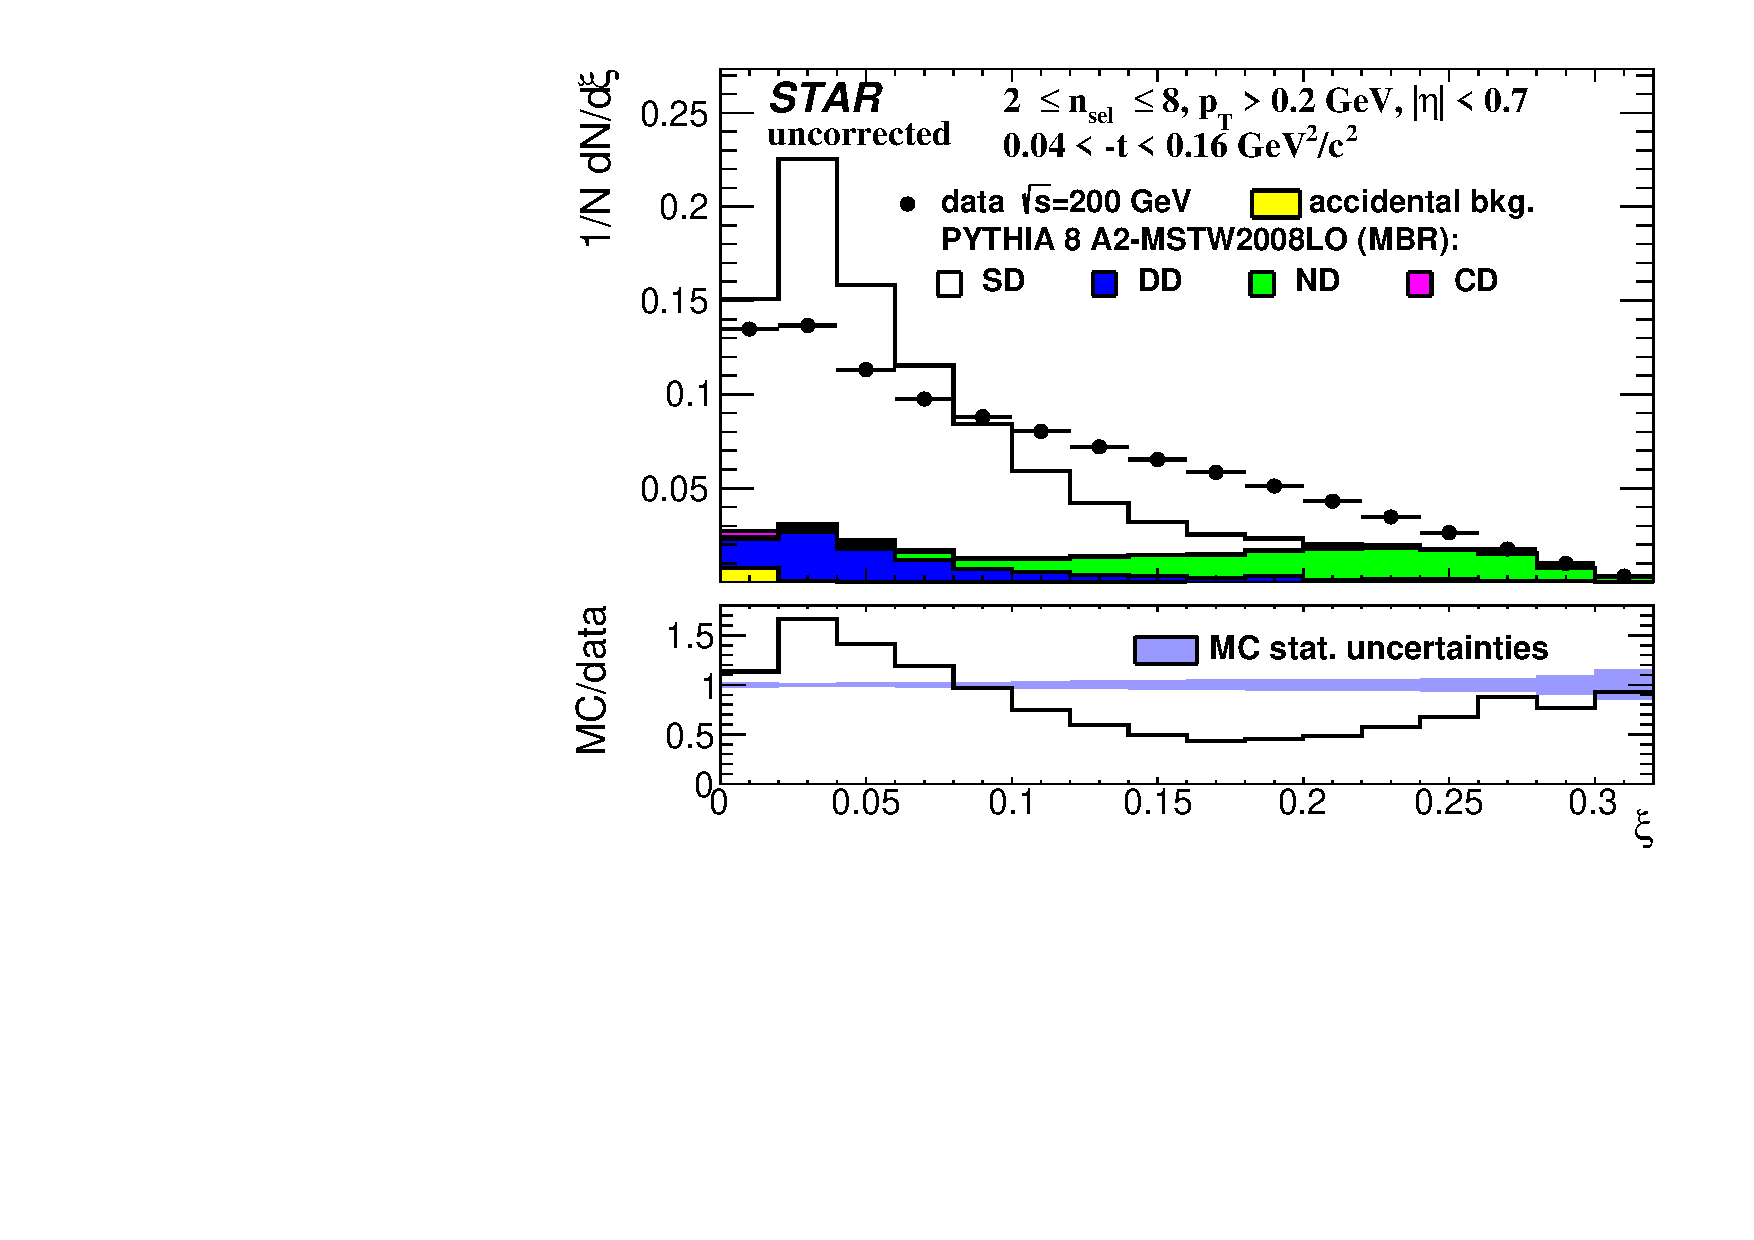
\includegraphics[width=.49\textwidth,page=1]{chapters/chrgSTAR/img/nonSD/SDT_pythia_xi0_RP_starsim_xi.pdf}
\hfill
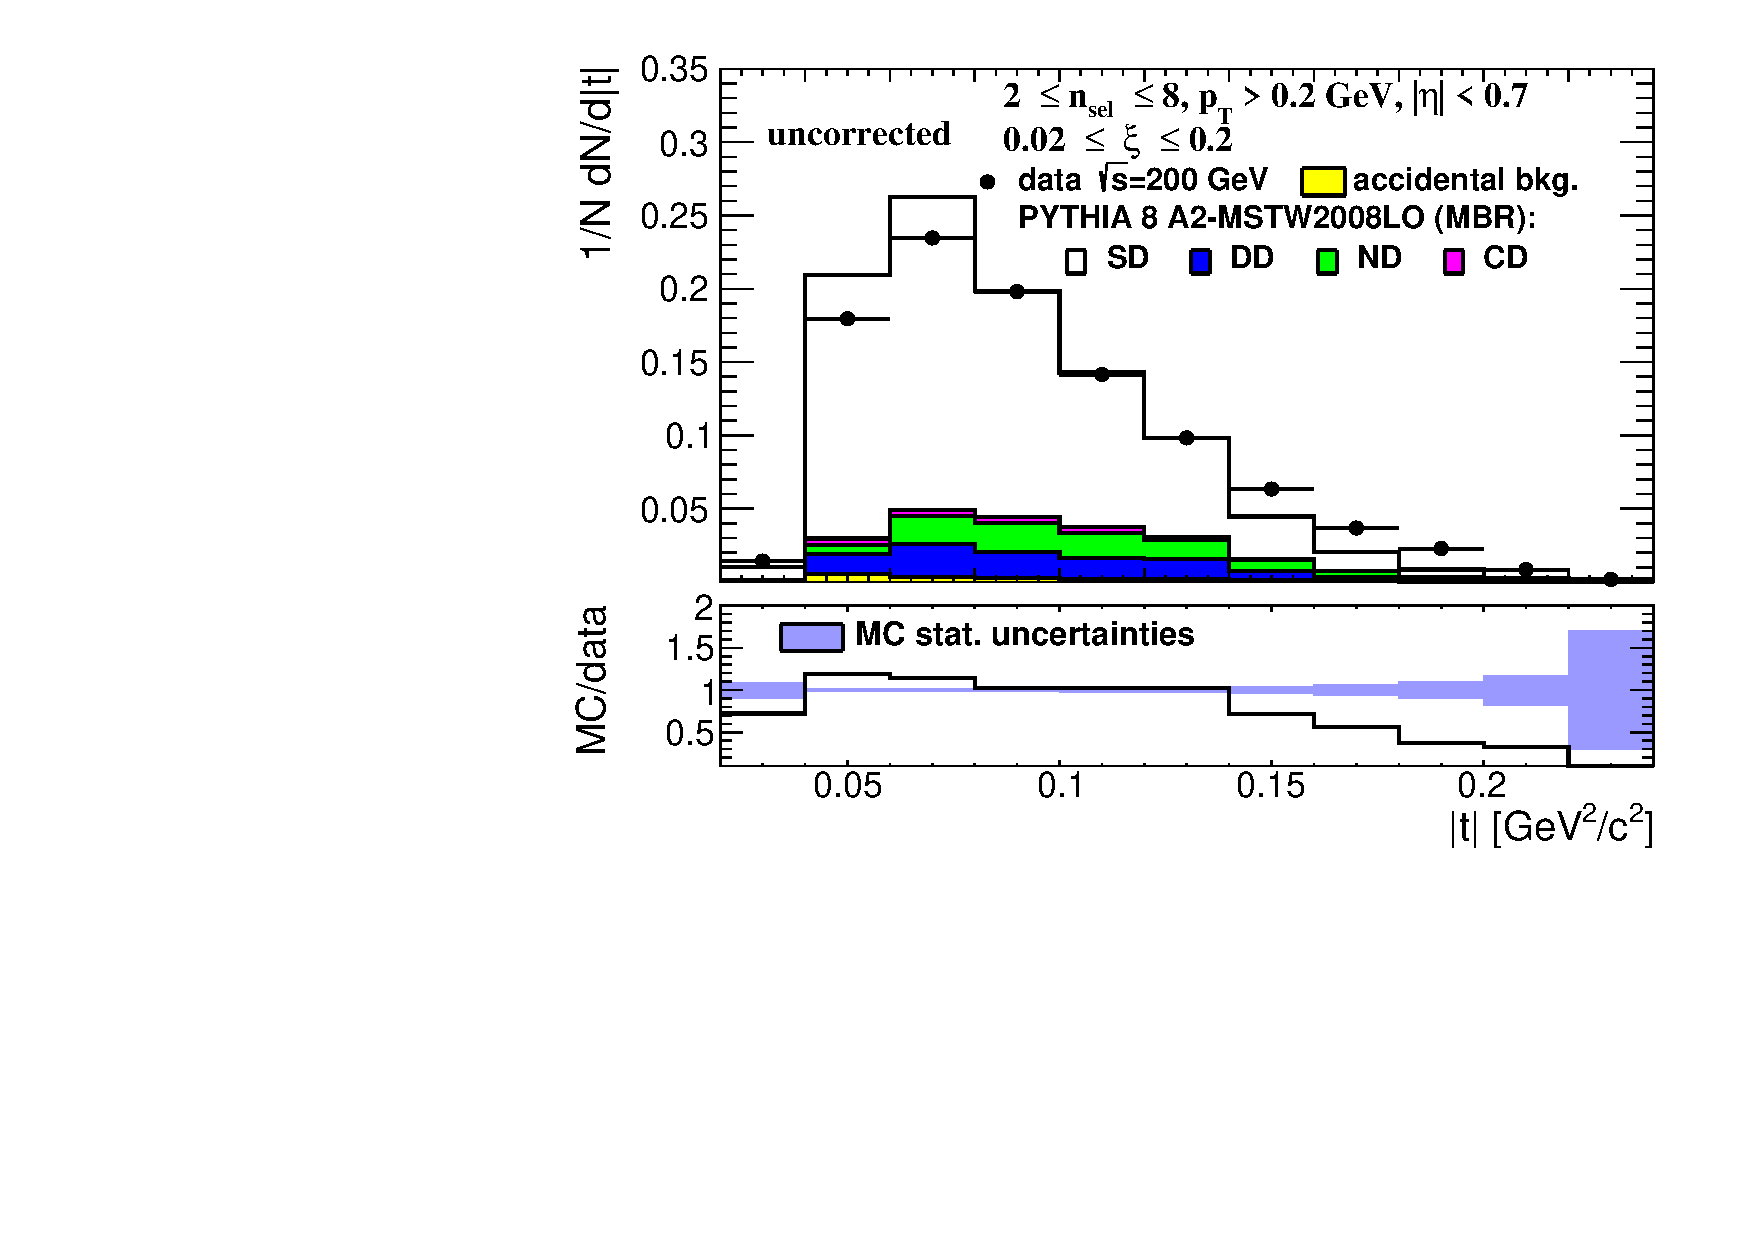
\includegraphics[width=.49\textwidth,page=1]{chapters/chrgSTAR/img/nonSD/SDT_pythia_xi0_RP_starsim_t.pdf}
\newline
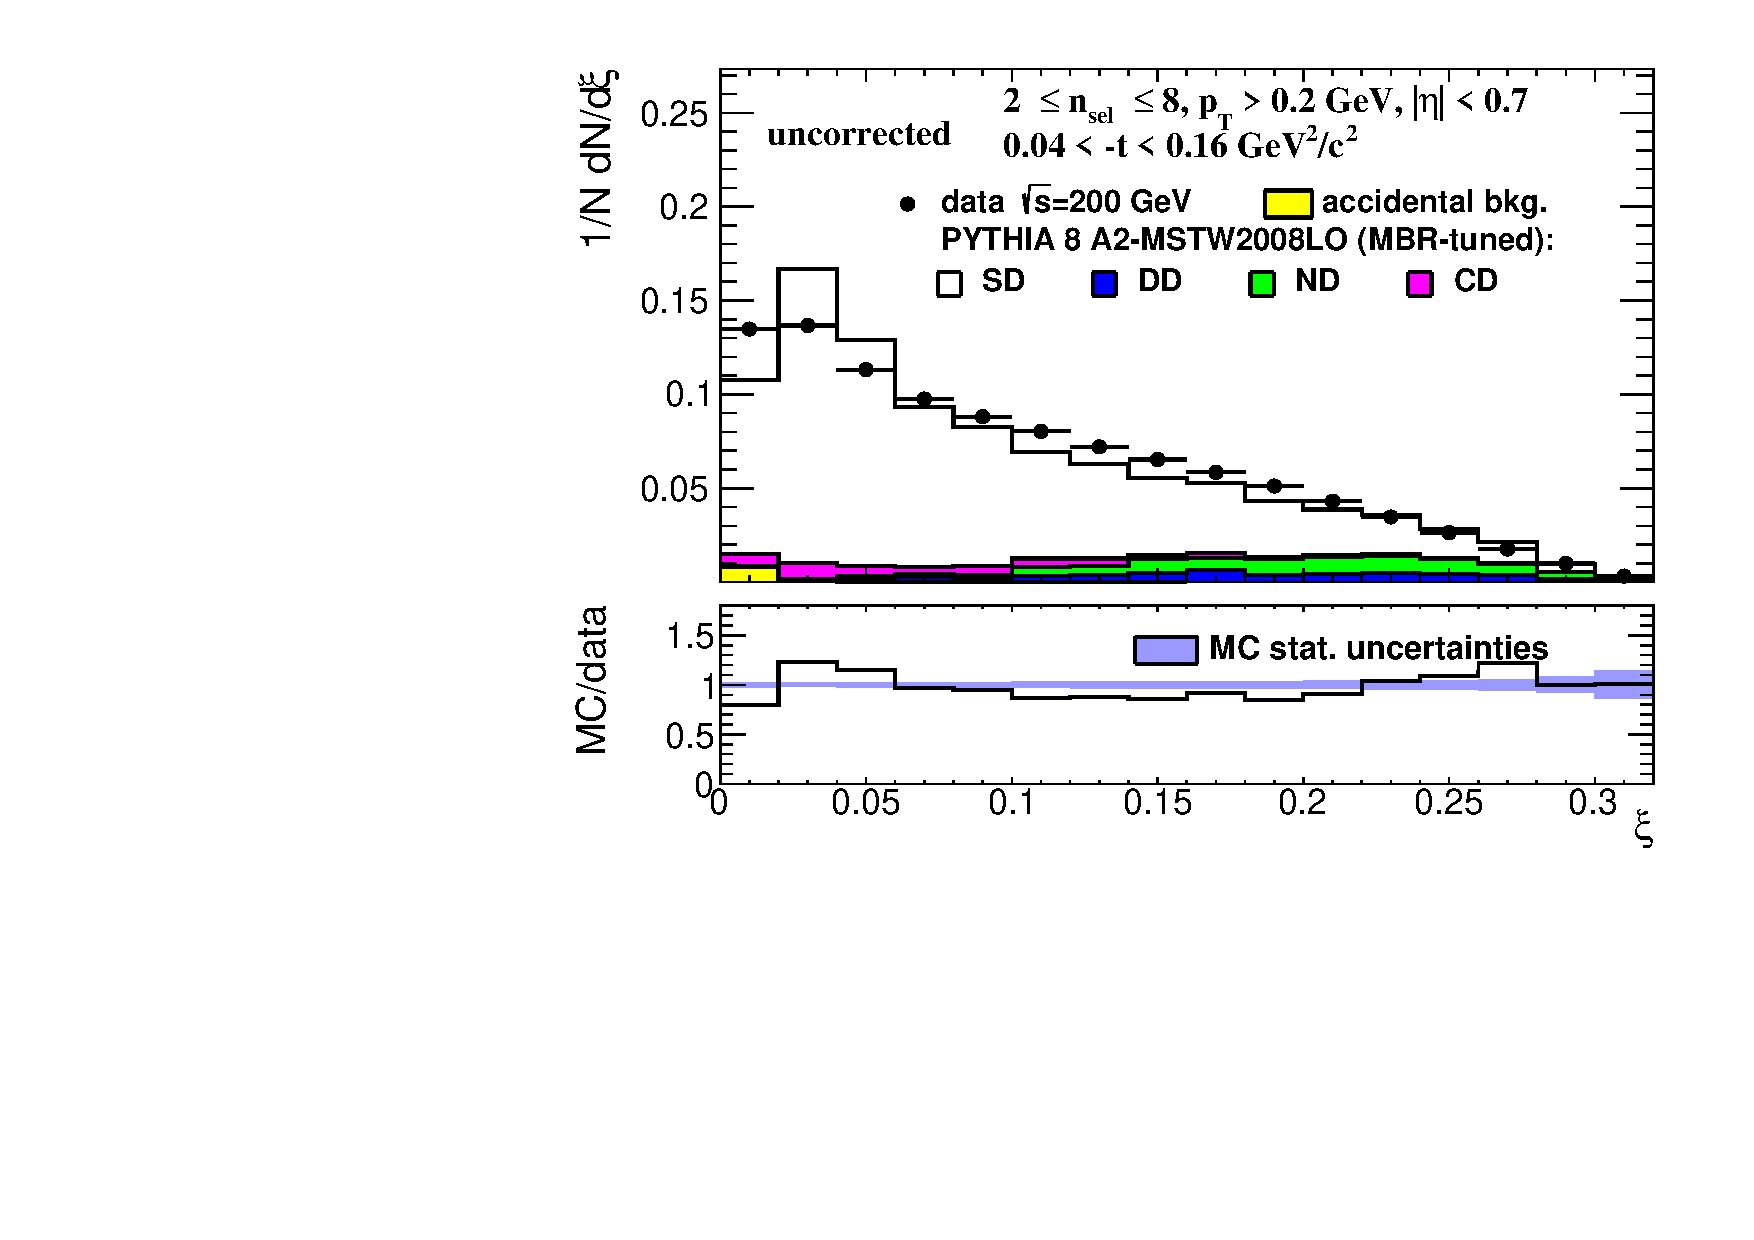
\includegraphics[width=.49\textwidth,page=1]{chapters/chrgSTAR/img/nonSD/SDT_pythia_xi0_option2_RP_starsim_xi.pdf}
\hfill
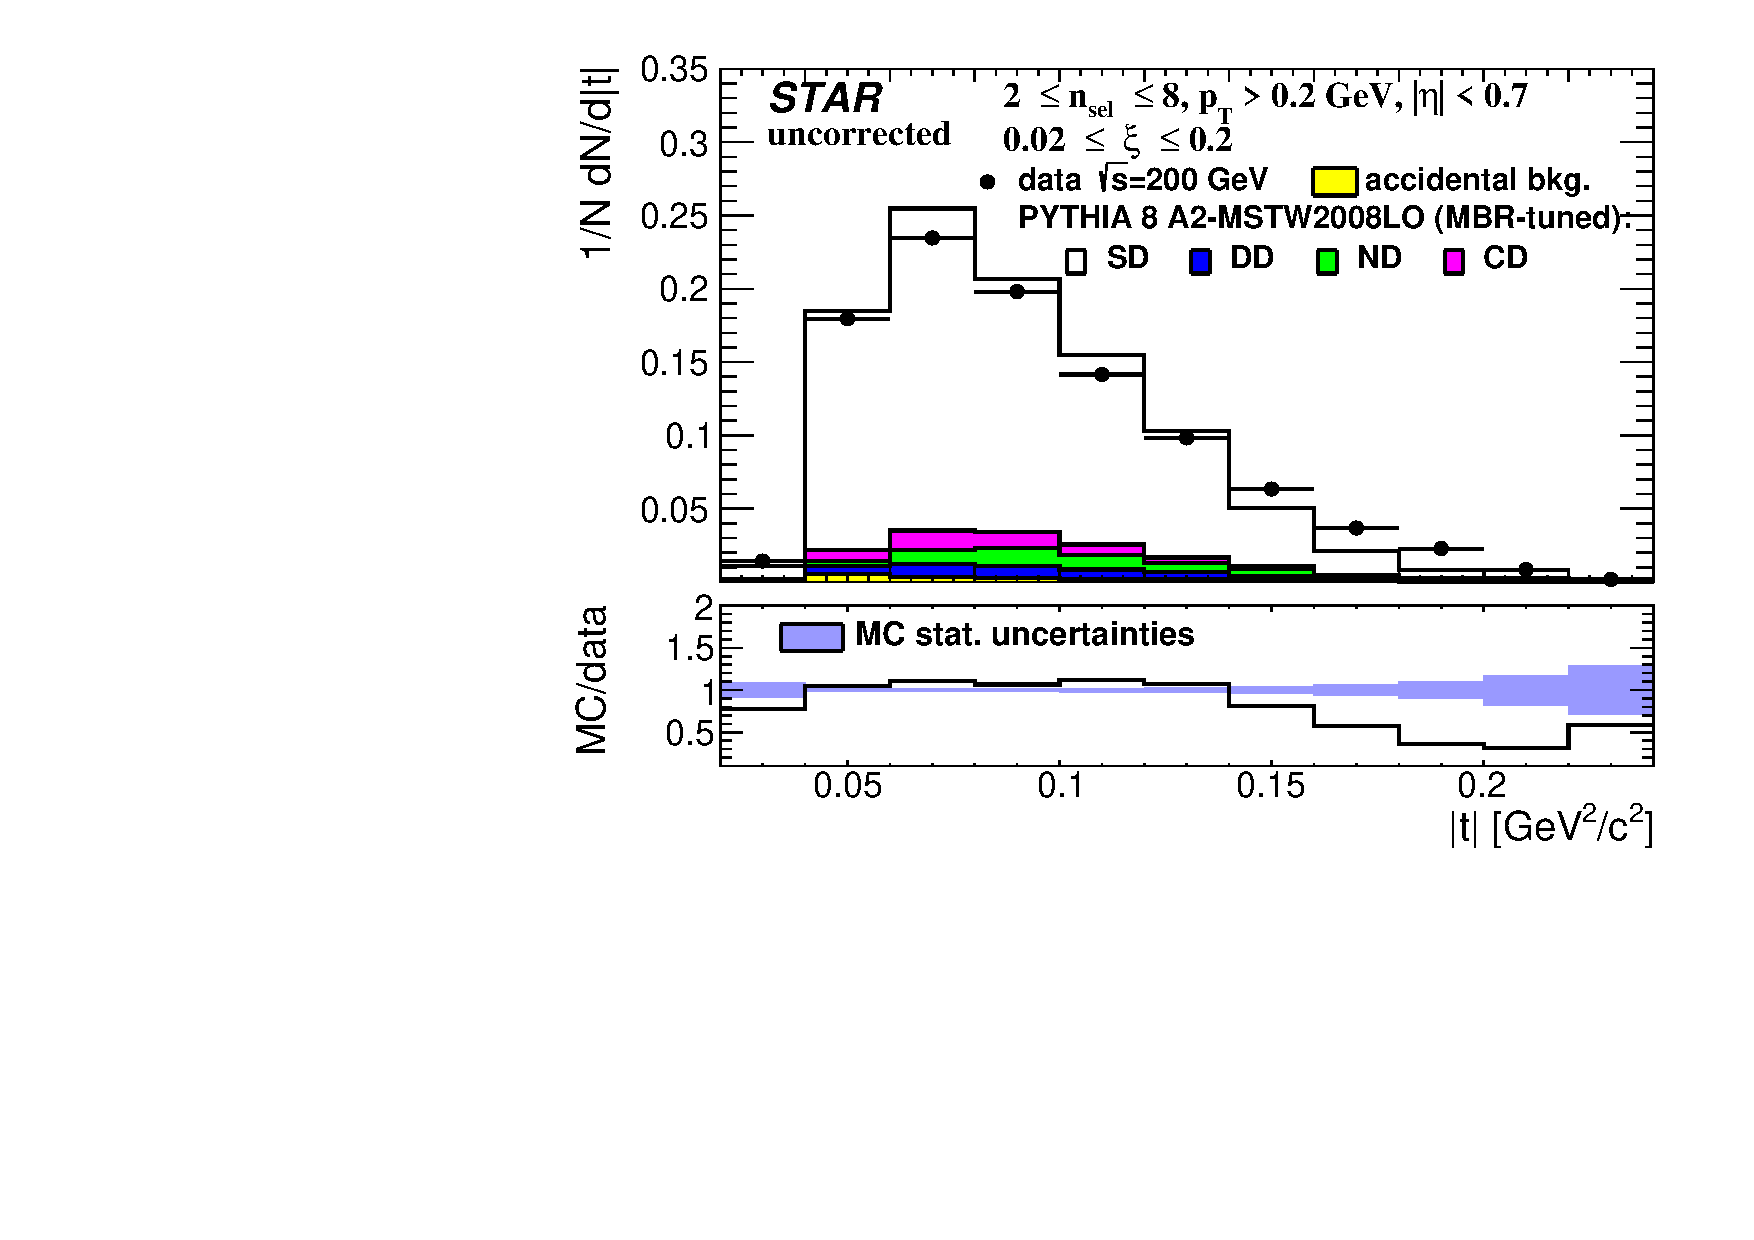
\includegraphics[width=.49\textwidth,page=1]{chapters/chrgSTAR/img/nonSD/SDT_pythia_xi0_option2_RP_starsim_t.pdf}
\newline
\includegraphics[width=.49\textwidth,page=1]{chapters/chrgSTAR/img/nonSD/SDT_epos_xi0_RP_starsim_xi.pdf}
\hfill
\includegraphics[width=.49\textwidth,page=1]{chapters/chrgSTAR/img/nonSD/SDT_epos_xi0_RP_starsim_t.pdf}
%
\caption{Uncorrected distributions of data compared to various MC models: (top) PYTHIA8 A2 (MBR), (middle) PYTHIA8 A2 (MBR-tuned) and (bottom) EPOS, as a function of (left column) $\xi$  and (right column) $|t|$.}
\label{fig:nonSDxit}
\end{figure}
\newpage

\begin{figure}[H]
\centering
\begin{subfigure}{.45\textwidth}
\includegraphics[width=\linewidth, page=1]{chapters/chrgSTAR/img/nonSD/chrg/SDT_pythia_xi0_RP_starsim_nsel.pdf}
\end{subfigure}
\begin{subfigure}{.45\textwidth}
\includegraphics[width=\linewidth, page=1]{chapters/chrgSTAR/img/nonSD/chrg/SDT_pythia_xi0_option2_RP_starsim_nsel.pdf}
\end{subfigure}
\begin{subfigure}{.45\textwidth}
\includegraphics[width=\linewidth, page=1]{chapters/chrgSTAR/img/nonSD/chrg/SDT_epos_xi0_RP_starsim_nsel.pdf}
\end{subfigure}
\begin{minipage}{.45\textwidth}
\caption{Uncorrected distributions of data compared to various MC models: (top left) PYTHIA8 A2 (MBR), (top right) PYTHIA8 A2 (MBR-tuned) and (bottom) EPOS, as a function of $n_{\mathrm{sel}}$.}
\label{fig:nonSDnsel}
\end{minipage}

\end{figure}
\begin{figure}[H]
%	\vspace{-0.5cm}
\centering
\begin{subfigure}{.45\textwidth}
\includegraphics[width=\linewidth, page=1]{chapters/chrgSTAR/img/nonSD/chrg/SDT_pythia_xi0_RP_starsim_pt.pdf}
\end{subfigure}
\begin{subfigure}{.45\textwidth}
\includegraphics[width=\linewidth, page=1]{chapters/chrgSTAR/img/nonSD/chrg/SDT_pythia_xi0_option2_RP_starsim_pt.pdf}
\end{subfigure}
\begin{subfigure}{.45\textwidth}
\includegraphics[width=\linewidth, page=1]{chapters/chrgSTAR/img/nonSD/chrg/SDT_epos_xi0_RP_starsim_pt.pdf}
\end{subfigure}
\begin{minipage}{.45\textwidth}
\caption{Uncorrected distributions of data compared to various MC models: (top left) PYTHIA8 A2 (MBR), (top right) PYTHIA8 A2 (MBR-tuned) and (bottom) EPOS, as a function of $p_{\mathrm{T}}$.}
\label{fig:nonSDpt}
\end{minipage}

\end{figure}
\newpage
\begin{figure}[H]
%	\vspace{-0.5cm}
\centering
\begin{subfigure}{.45\textwidth}
\includegraphics[width=\linewidth, page=1]{chapters/chrgSTAR/img/nonSD/chrg/SDT_pythia_xi0_RP_starsim_eta.pdf}
\end{subfigure}
\begin{subfigure}{.45\textwidth}
\includegraphics[width=\linewidth, page=1]{chapters/chrgSTAR/img/nonSD/chrg/SDT_pythia_xi0_option2_RP_starsim_eta.pdf}
\end{subfigure}
\begin{subfigure}{.45\textwidth}
\includegraphics[width=\linewidth, page=1]{chapters/chrgSTAR/img/nonSD/chrg/SDT_epos_xi0_RP_starsim_eta.pdf}
\end{subfigure}
\begin{minipage}{.45\textwidth}
\caption{Uncorrected distributions of data compared to various MC models: (top left) PYTHIA8 A2 (MBR), (top right) PYTHIA8 A2 (MBR-tuned) and (bottom) EPOS, as a function of $\bar{\eta}$. }
\label{fig:nonSDera}
\end{minipage}

\end{figure}
\end{comment}
Events, in which  forward-scattered proton and reconstructed TOF
vertex are the result of the same $pp$ interaction, may originate from \ac{ND}, \ac{DD}, \ac{SD}, and \ac{CD} processes.  It is preferred to estimate the~background contribution from data, using dedicated control regions.
Since such regions were not found, the~relative contributions from the~above processes were  estimated from MC models and are therefore model dependent. Tracks reconstructed in \ac{RP}s  %which are modeled in the~\ac{MC} simulations are only coming from:
may also be:
\begin{itemize}
	\item forward-scattered protons produced in the \ac{SD}, \ac{CD} or \ac{DD} diffractive systems or from \ac{ND} events,
	\item secondary particles from showering initiated 
	by interaction of forward-scattered protons with beam-line elements. This contribution is negligible.
\end{itemize}


Figure~\ref{fig:nonSDxit} shows the uncorrected $\xi$ and $t$ distributions in data compared to various \ac{MC} models: PYTHIA~8 A2 (MBR), PYTHIA~8 A2 (MBR-tuned), PYTHIA~8 4C (SaS) and EPOS. The \ac{MC} distributions are split into \ac{SD}, \ac{ND}, \ac{DD} and \ac{CD} components. For EPOS, SD$^\prime$ is separated from the ND events. Additionally, the accidental background is also shown. PYTHIA~8 A2 (MBR) predictions, shown in Fig.~\ref{fig:nonSDxit} (a-b), do not agree with the data, especially  there is small number of events in the~region of large values of $\xi$. 
This effect may be due to the~scaling factors, which are introduced in PYTHIA~8 to artificially suppress diffractive cross sections in the~high mass region, or due to too large Pomeron intercept ($\epsilon=0.104$).
 Therefore,
additional two samples of PYTHIA~8 were generated: without this artificial suppression  (\mbox{MBR-tuned}) and with  $\epsilon=0$ (\mbox{SaS}). Their predictions, shown in Fig.~\ref{fig:nonSDxit} (c-f), agree much better with the~data than PYTHIA~8 A2 (MBR) and result also in a~suppression of non-SD events. Amongst PYTHIA~8 models, PYTHIA~8 A2 (MBR-tuned) shows the~best agreement  with the~data.
EPOS predictions,  shown in Fig.~\ref{fig:nonSDxit} (g-h), describes data better than PYTHIA~8 but shows a dominant contribution of SD$^\prime$ events. The~CD contribution in EPOS is several times greater than in PYTHIA~8 (MBR), but it was never tuned to describe any data, as opposed to PYTHIA~8 (MBR) in which the~\ac{CD} cross sections are constrained by CDF measurements~\cite{Acosta:2003xi}. 
The~\ac{CD} component in the~\ac{SaS} model is based on simple scaling assumption, therefore, it is not usually used by the~experimental communities. All MCs predict significant \ac{DD} and \ac{ND} background at large $\xi$, thereby  the analysis was limited to $\xi < 0.2$. 


\Cref{fig:nonSDnsel,fig:nonSDpt,fig:nonSDera} show the uncorrected distributions of variables used in the later analysis: $n_{\mathrm{sel}}$, $p_{\mathrm T}$ an $\bar{\eta}$. The  contributions from non-SD (except  EPOS SD$^\prime$) interactions differ a bit between each other, i.e. EPOS predicts significantly larger CD contribution, whereas DD and ND are suppressed in PYTHIA~8 A2 (MBR-tuned) and PYTHIA~8 4C (SaS).  PYTHIA~8~A2~(MBR) is used as the default model  of non-SD contribution subtracted from the data with systematic uncertainty $\pm50\%$, which covers all differences between the~models except EPOS SD$^\prime$.  In this analysis EPOS SD$^\prime$ is   considered as an~alternative to PYTHIA~8 SD model of events with forward-scattered proton in the final state,  where one of the proton remnants hadronizes back to a~single proton (non-diffractive process), while in  PYTHIA~8 the~initial proton stays intact (diffractive process). As a~consequence, results  are compared  with the~sum of SD and SD$^\prime$ processes for EPOS model.  
%\end{comment}
%\thispagestyle{empty}

%\newpage
\begin{figure}[H]
	%\vspace{-1.cm}
	\thisfloatpagestyle{fancy}
	\centering
	\begin{overpic}[width=0.47\textwidth,tics=4,page=1]{chapters/chrgSTAR/img/nonSD/SDT_pythia_xi0_RP_starsim_xi.pdf}
		\put (88,40) {\Large{a}}
	\end{overpic}
	\vspace{-0.2cm}
	\begin{overpic}[width=0.47\textwidth,tics=4,page=1]{chapters/chrgSTAR/img/nonSD/SDT_pythia_xi0_RP_starsim_t.pdf}
		\put (85,35) {\Large{b}}
	\end{overpic}
	\begin{overpic}[width=0.47\textwidth,tics=4,page=1]{chapters/chrgSTAR/img/nonSD/SDT_pythia_xi0_option2_RP_starsim_xi.pdf}
		\put (85,35) {\Large{c}}
	\end{overpic}
	\vspace{-0.2cm}
	\begin{overpic}[width=0.47\textwidth,tics=4,page=1]{chapters/chrgSTAR/img/nonSD/SDT_pythia_xi0_option2_RP_starsim_t.pdf}
		\put (85,35) {\Large{d}}
	\end{overpic}
	\begin{overpic}[width=0.47\textwidth,tics=4,page=1]{chapters/chrgSTAR/img/nonSD/SDT_pythia_xi0_sas_RP_starsim_xi.pdf}
		\put (85,35) {\Large{e}}
	\end{overpic}
	\vspace{-0.2cm}
	\begin{overpic}[width=0.47\textwidth,tics=4,page=1]{chapters/chrgSTAR/img/nonSD/SDT_pythia_xi0_sas_RP_starsim_t.pdf}
		\put (85,35) {\Large{f}}
	\end{overpic}
	\begin{overpic}[width=0.47\textwidth,tics=4,page=1]{chapters/chrgSTAR/img/nonSD/SDT_epos_xi0_RP_starsim_xi.pdf}
		\put (85,35) {\Large{g}}
	\end{overpic}
	\vspace{-0.2cm}
	\begin{overpic}[width=0.47\textwidth,tics=4,page=1]{chapters/chrgSTAR/img/nonSD/SDT_epos_xi0_RP_starsim_t.pdf}
		\put (85,35) {\Large{h}}
	\end{overpic}
	\vspace{-0.2cm}
	%
	\caption{Uncorrected distributions of data compared to various MC models: (a-b) PYTHIA~8 A2 (MBR), (c-d) PYTHIA~8 A2 (MBR-tuned), (e-f) PYTHIA~8 4C (SaS) and (g-h) EPOS, as a~function of (left column) $\xi$  and (right column) $|t|$. The~ratio of MC predictions and data is shown in the~bottom panels.}
	\label{fig:nonSDxit}
	%\vspace{-0.5cm}
\end{figure}

\begin{figure}[t!]
	\vspace{-1.5cm}
	\thisfloatpagestyle{fancy}
	\centering
	\begin{subfigure}{.49\textwidth}
		\includegraphics[width=\linewidth, page=1]{chapters/chrgSTAR/img/nonSD/chrg/SDT_pythia_xi0_RP_starsim_nsel.pdf}
	\end{subfigure}
	\begin{subfigure}{.49\textwidth}
		\includegraphics[width=\linewidth, page=1]{chapters/chrgSTAR/img/nonSD/chrg/SDT_pythia_xi0_option2_RP_starsim_nsel.pdf}
	\end{subfigure}
	\begin{subfigure}{.49\textwidth}
		\includegraphics[width=\linewidth, page=1]{chapters/chrgSTAR/img/nonSD/SDT_pythia_xi0_sas_RP_starsim_nsel.pdf}
	\end{subfigure}
	\begin{subfigure}{.49\textwidth}
		\includegraphics[width=\linewidth, page=1]{chapters/chrgSTAR/img/nonSD/chrg/SDT_epos_xi0_RP_starsim_nsel.pdf}
	\end{subfigure}
	%\begin{minipage}{.49\textwidth}
	\caption{Uncorrected distributions of data compared to various MC models: (top left) PYTHIA~8 A2 (MBR), (top right) PYTHIA~8 A2 (MBR-tuned), (bottom left) PYTHIA~8 4C (SaS) and (bottom right) EPOS, as a function of $n_{\mathrm{sel}}$. The~ratio of MC predictions and data is shown in the~bottom panels.}
	\label{fig:nonSDnsel}
	%\end{minipage}
	
%\end{figure}

%\begin{figure}[t!]
	%\vspace{-0.5cm}
	\centering
	\begin{subfigure}{.49\textwidth}
		\includegraphics[width=\linewidth, page=1]{chapters/chrgSTAR/img/nonSD/chrg/SDT_pythia_xi0_RP_starsim_pt.pdf}
	\end{subfigure}
	\begin{subfigure}{.49\textwidth}
		\includegraphics[width=\linewidth, page=1]{chapters/chrgSTAR/img/nonSD/chrg/SDT_pythia_xi0_option2_RP_starsim_pt.pdf}
	\end{subfigure}
	\begin{subfigure}{.49\textwidth}
		\includegraphics[width=\linewidth, page=1]{chapters/chrgSTAR/img/nonSD/SDT_pythia_xi0_sas_RP_starsim_pt.pdf}
	\end{subfigure}
	\begin{subfigure}{.49\textwidth}
		\includegraphics[width=\linewidth, page=1]{chapters/chrgSTAR/img/nonSD/chrg/SDT_epos_xi0_RP_starsim_pt.pdf}
	\end{subfigure}
	%\begin{minipage}{.49\textwidth}
		\caption{Uncorrected distributions of data compared to various MC models: (top left) PYTHIA~8 A2 (MBR), (top right) PYTHIA~8 A2 (MBR-tuned), (bottom left) PYTHIA~8 4C (SaS) and (bottom right) EPOS, as a function of $p_{\mathrm{T}}$. The~ratio of MC predictions and data is shown in the~bottom panels.}
		\label{fig:nonSDpt}
	%\end{minipage}
	%\vspace{-0.5cm}
\end{figure}
%\newpage
\begin{figure}[t!]
	%	\vspace{-0.5cm}
	\thisfloatpagestyle{fancy}
	\centering
	\begin{subfigure}{.49\textwidth}
		\includegraphics[width=\linewidth, page=1]{chapters/chrgSTAR/img/nonSD/chrg/SDT_pythia_xi0_RP_starsim_eta.pdf}
	\end{subfigure}
	\begin{subfigure}{.49\textwidth}
		\includegraphics[width=\linewidth, page=1]{chapters/chrgSTAR/img/nonSD/chrg/SDT_pythia_xi0_option2_RP_starsim_eta.pdf}
	\end{subfigure}
	\begin{subfigure}{.49\textwidth}
		\includegraphics[width=\linewidth, page=1]{chapters/chrgSTAR/img/nonSD/SDT_pythia_xi0_sas_RP_starsim_eta.pdf}
	\end{subfigure}
	\begin{subfigure}{.49\textwidth}
		\includegraphics[width=\linewidth, page=1]{chapters/chrgSTAR/img/nonSD/chrg/SDT_epos_xi0_RP_starsim_eta.pdf}
	\end{subfigure}
	%\begin{minipage}{.49\textwidth}
		\caption{Uncorrected distributions of data compared to various MC models: (top left) PYTHIA~8 A2 (MBR), (top right) PYTHIA~8 A2 (MBR-tuned), (bottom left) PYTHIA~8 4C (SaS) and (bottom right) EPOS, as a function of $\bar{\eta}$. The~ratio of MC predictions and data is shown in the~bottom panels.}
		\label{fig:nonSDera}
	%\end{minipage}
	
\end{figure}
%\end{comment}
%\FloatBarrier
%background non primary
\section{Background from Non-Primary Tracks}\label{section:star_background_primary}
Reconstructed tracks matched to a~non-primary particle, so-called background tracks,  originate  mainly from the~following sources:
\begin{itemize}
	\item decays of short-lived primary particles with strange quark content (mostly $K^0$, $\Lambda^0$),
	\item photons from $\pi^0$ and $\eta$ decays which are converting to $e^+e^-$,
	\item hadronic interactions of particles with the beam-pipe or detector dead material.
\end{itemize} 

\begin{figure}[b!]
	\centering
	\begin{subfigure}{.49\textwidth}
		\includegraphics[width=\linewidth, page=1]{chapters/chrgSTAR/img/chargedBkg/bkg2D.pdf}
	\end{subfigure}
	\begin{subfigure}{.49\textwidth}
		\includegraphics[width=\linewidth, page=7]{chapters/chrgSTAR/img/chargedBkg/bkg2D_epos.pdf}
	\end{subfigure}
	\begin{comment}
	\begin{subfigure}{.45\textwidth}
	\includegraphics[width=\linewidth, page=4]{chapters/chrgSTAR/img/chargedBkg/bkg2D.pdf}
	\end{subfigure}
	\begin{subfigure}{.45\textwidth}
	\includegraphics[width=\linewidth, page=5]{chapters/chrgSTAR/img/chargedBkg/bkg2D.pdf}
	\end{subfigure}
	\end{comment}
	\caption{Distribution of fraction of selected tracks  associated with non-primary particles  in the~range $0.02<\xi<0.2$ as predicted by (left) PYTHIA~8 4C (SaS) embedding and (right) EPOS SD+SD$^\prime$.}
	\label{fig:bkg_fake_charged}
\end{figure}
Figure~\ref{fig:bkg_fake_charged} (left) shows the background from non-primary tracks, $f_{\textrm{bkg}}\left(p_{\textrm{T}},\eta\right)$, %and fake track $f_{\textrm{fake}}\left(p_{\textrm{T}},\eta\right)$ contribution to reconstructed tracks 
as a~function of tracks' $p_{\textrm{T}}$ and $\eta$, predicted by PYTHIA~8 SD model. There were no differences observed in the~background contribution in different $\xi$ ranges, hence, all three $\xi$ ranges were merged for this study. The highest background fraction, which varies between $5-10\%$, was found to be at low $p_{\textrm{T}}$.  %Due to too low statistics in PYTHIA~8 embedding \ac{MC}, the~shape of the~fake track contribution was assumed to be the~same in all three $\xi$ ranges. However, its normalization was calculated for each $\xi$ range separately with a ratio between the ranges of $1: 0.74: 1.11$.


Figure~\ref{fig:bkg_fake_charged} (right) shows the~background track contribution to reconstructed tracks as a~function of $p_\textrm{T}$ and $\eta$ calculated from EPOS SD+SD$^\prime$. The differences between
PYTHIA~8 and EPOS, which are up to $50\%$ for $p_\textrm{T}>0.5$~GeV/c (as shown in Fig.~\ref{fig:bkg_epos_charged_1D}), were symmetrized and taken as a~systematic uncertainty.

There is also a~small ($<0.5\%$) contribution from fake tracks, $f_{\textrm{fake}}\left(p_{\textrm{T}},\eta\right)$, i.e. tracks not associated with true-level particles, coming from out-of-time pile-up or  formed by a~random combination of TPC hits. The~change by $\pm100\%$ in this contribution was taken as a systematic uncertainty.

\begin{figure}[t!]
	\centering
	\begin{subfigure}{.49\textwidth}
		\includegraphics[width=\linewidth, page=8]{chapters/chrgSTAR/img/chargedBkg/bkg2D.pdf}
	\end{subfigure}
	\begin{subfigure}{.49\textwidth}
		\includegraphics[width=\linewidth, page=9]{chapters/chrgSTAR/img/chargedBkg/bkg2D.pdf}
	\end{subfigure}
	\vspace{-0.25cm}
	\caption{PYTHIA~8 SD and EPOS SD+SD$^\prime$ predictions of fraction of selected tracks  associated with non-primary particles  as a~function of (left) $p_\textrm{T}$ and (right) $\eta$. The~ratio of EPOS and PYTHIA~8 predictions is shown in the~bottom panels.}
	\label{fig:bkg_epos_charged_1D}
	\vspace{-0.25cm}
\end{figure}

%\FloatBarrier
%background proton
\input{chapters/chrgSTAR/backgroundProton.tex}
%background pion
\input{chapters/chrgSTAR/backgroundPion.tex}

% !TeX spellcheck = en_GB
\section{Control Plots}\label{section:star_nonSD}
\begin{comment}
The background contributions coming from \ac{ND}, \ac{DD} and \ac{CD} events are estimated from \ac{MC} simulations. Protons from elastic interactions and beam halo are not included in the~simulation. \ac{SD} background signatures which are modeled in th~\ac{MC} simulations are only coming from :
\begin{itemize}
\item forward protons produced in the \ac{SD}, \ac{CD} or \ac{DD} diffractive systems or through non-diffractive  \ac{QCD},
\item reconstructed tracks coming from showering.
\end{itemize}

Figure~\ref{fig:nonSDxit} shows the uncorrected $\xi$ and $t$ distributions in data compared to various \ac{MC} models: PYTHIA 8 A2 (MBR), PYTHIA 8 A2 (MBR-tuned) and EPOS. The \ac{MC} distributions are split into \ac{SD}, \ac{ND}, \ac{DD} and \ac{CD} components. For EPOS low mass excitation of the proton remnant (SD') is separated from the ND events. Additionally, the accidental background is also shown. Without arbitrary suppression of diffractive cross sections at large $\xi$ PYTHIA8 A2 (MBR-tuned) predictions agree much better with the data and result also in a suppression of non-SD events. EPOS describes data better than PYTHIA8 but shows a dominant contribution of SD' events. All MCs predict significant non-SD background at large $\xi$, thereby  the analysis was limited to $\xi < 0.2$. 

On the other hand, \cref{fig:nonSDnsel,fig:nonSDpt,fig:nonSDera} show the uncorrected distributions of variables used in the later analysis: $n_{\mathrm{sel}}$, $p_{\mathrm T}$ an $\bar{\eta}$. The background contributions from non-SD interactions differ a bit between each other, i.e. EPOS predicts significantly larger CD contribution, whereas DD and ND are suppressed in PYTHIA 8 A2 (MBR-tuned).  As a result PYTHIA~8~A2~(MBR) is used as the default model  of non-SD with systematic uncertainty $\pm50\%$, which covers all differences between the~models. %Moreover, SD' in EPOS was not subtracted but used separately for comparisons.

\begin{figure}[H]
\centering
\includegraphics[width=.49\textwidth,page=1]{chapters/chrgSTAR/img/nonSD/SDT_pythia_xi0_RP_starsim_xi.pdf}
\hfill
\includegraphics[width=.49\textwidth,page=1]{chapters/chrgSTAR/img/nonSD/SDT_pythia_xi0_RP_starsim_t.pdf}
\newline
\includegraphics[width=.49\textwidth,page=1]{chapters/chrgSTAR/img/nonSD/SDT_pythia_xi0_option2_RP_starsim_xi.pdf}
\hfill
\includegraphics[width=.49\textwidth,page=1]{chapters/chrgSTAR/img/nonSD/SDT_pythia_xi0_option2_RP_starsim_t.pdf}
\newline
\includegraphics[width=.49\textwidth,page=1]{chapters/chrgSTAR/img/nonSD/SDT_epos_xi0_RP_starsim_xi.pdf}
\hfill
\includegraphics[width=.49\textwidth,page=1]{chapters/chrgSTAR/img/nonSD/SDT_epos_xi0_RP_starsim_t.pdf}
%
\caption{Uncorrected distributions of data compared to various MC models: (top) PYTHIA8 A2 (MBR), (middle) PYTHIA8 A2 (MBR-tuned) and (bottom) EPOS, as a function of (left column) $\xi$  and (right column) $|t|$.}
\label{fig:nonSDxit}
\end{figure}
\newpage

\begin{figure}[H]
\centering
\begin{subfigure}{.45\textwidth}
\includegraphics[width=\linewidth, page=1]{chapters/chrgSTAR/img/nonSD/chrg/SDT_pythia_xi0_RP_starsim_nsel.pdf}
\end{subfigure}
\begin{subfigure}{.45\textwidth}
\includegraphics[width=\linewidth, page=1]{chapters/chrgSTAR/img/nonSD/chrg/SDT_pythia_xi0_option2_RP_starsim_nsel.pdf}
\end{subfigure}
\begin{subfigure}{.45\textwidth}
\includegraphics[width=\linewidth, page=1]{chapters/chrgSTAR/img/nonSD/chrg/SDT_epos_xi0_RP_starsim_nsel.pdf}
\end{subfigure}
\begin{minipage}{.45\textwidth}
\caption{Uncorrected distributions of data compared to various MC models: (top left) PYTHIA8 A2 (MBR), (top right) PYTHIA8 A2 (MBR-tuned) and (bottom) EPOS, as a function of $n_{\mathrm{sel}}$.}
\label{fig:nonSDnsel}
\end{minipage}

\end{figure}
\begin{figure}[H]
%	\vspace{-0.5cm}
\centering
\begin{subfigure}{.45\textwidth}
\includegraphics[width=\linewidth, page=1]{chapters/chrgSTAR/img/nonSD/chrg/SDT_pythia_xi0_RP_starsim_pt.pdf}
\end{subfigure}
\begin{subfigure}{.45\textwidth}
\includegraphics[width=\linewidth, page=1]{chapters/chrgSTAR/img/nonSD/chrg/SDT_pythia_xi0_option2_RP_starsim_pt.pdf}
\end{subfigure}
\begin{subfigure}{.45\textwidth}
\includegraphics[width=\linewidth, page=1]{chapters/chrgSTAR/img/nonSD/chrg/SDT_epos_xi0_RP_starsim_pt.pdf}
\end{subfigure}
\begin{minipage}{.45\textwidth}
\caption{Uncorrected distributions of data compared to various MC models: (top left) PYTHIA8 A2 (MBR), (top right) PYTHIA8 A2 (MBR-tuned) and (bottom) EPOS, as a function of $p_{\mathrm{T}}$.}
\label{fig:nonSDpt}
\end{minipage}

\end{figure}
\newpage
\begin{figure}[H]
%	\vspace{-0.5cm}
\centering
\begin{subfigure}{.45\textwidth}
\includegraphics[width=\linewidth, page=1]{chapters/chrgSTAR/img/nonSD/chrg/SDT_pythia_xi0_RP_starsim_eta.pdf}
\end{subfigure}
\begin{subfigure}{.45\textwidth}
\includegraphics[width=\linewidth, page=1]{chapters/chrgSTAR/img/nonSD/chrg/SDT_pythia_xi0_option2_RP_starsim_eta.pdf}
\end{subfigure}
\begin{subfigure}{.45\textwidth}
\includegraphics[width=\linewidth, page=1]{chapters/chrgSTAR/img/nonSD/chrg/SDT_epos_xi0_RP_starsim_eta.pdf}
\end{subfigure}
\begin{minipage}{.45\textwidth}
\caption{Uncorrected distributions of data compared to various MC models: (top left) PYTHIA8 A2 (MBR), (top right) PYTHIA8 A2 (MBR-tuned) and (bottom) EPOS, as a function of $\bar{\eta}$. }
\label{fig:nonSDera}
\end{minipage}

\end{figure}
\end{comment}
Events, in which  forward-scattered proton and reconstructed TOF
vertex are the result of the same $pp$ interaction, may originate from \ac{ND}, \ac{DD}, \ac{SD}, and \ac{CD} processes.  It is preferred to estimate the~background contribution from data, using dedicated control regions.
Since such regions were not found, the~relative contributions from the~above processes were  estimated from MC models and are therefore model dependent. Tracks reconstructed in \ac{RP}s  %which are modeled in the~\ac{MC} simulations are only coming from:
may also be:
\begin{itemize}
	\item forward-scattered protons produced in the \ac{SD}, \ac{CD} or \ac{DD} diffractive systems or from \ac{ND} events,
	\item secondary particles from showering initiated 
	by interaction of forward-scattered protons with beam-line elements. This contribution is negligible.
\end{itemize}


Figure~\ref{fig:nonSDxit} shows the uncorrected $\xi$ and $t$ distributions in data compared to various \ac{MC} models: PYTHIA~8 A2 (MBR), PYTHIA~8 A2 (MBR-tuned), PYTHIA~8 4C (SaS) and EPOS. The \ac{MC} distributions are split into \ac{SD}, \ac{ND}, \ac{DD} and \ac{CD} components. For EPOS, SD$^\prime$ is separated from the ND events. Additionally, the accidental background is also shown. PYTHIA~8 A2 (MBR) predictions, shown in Fig.~\ref{fig:nonSDxit} (a-b), do not agree with the data, especially  there is small number of events in the~region of large values of $\xi$. 
This effect may be due to the~scaling factors, which are introduced in PYTHIA~8 to artificially suppress diffractive cross sections in the~high mass region, or due to too large Pomeron intercept ($\epsilon=0.104$).
 Therefore,
additional two samples of PYTHIA~8 were generated: without this artificial suppression  (\mbox{MBR-tuned}) and with  $\epsilon=0$ (\mbox{SaS}). Their predictions, shown in Fig.~\ref{fig:nonSDxit} (c-f), agree much better with the~data than PYTHIA~8 A2 (MBR) and result also in a~suppression of non-SD events. Amongst PYTHIA~8 models, PYTHIA~8 A2 (MBR-tuned) shows the~best agreement  with the~data.
EPOS predictions,  shown in Fig.~\ref{fig:nonSDxit} (g-h), describes data better than PYTHIA~8 but shows a dominant contribution of SD$^\prime$ events. The~CD contribution in EPOS is several times greater than in PYTHIA~8 (MBR), but it was never tuned to describe any data, as opposed to PYTHIA~8 (MBR) in which the~\ac{CD} cross sections are constrained by CDF measurements~\cite{Acosta:2003xi}. 
The~\ac{CD} component in the~\ac{SaS} model is based on simple scaling assumption, therefore, it is not usually used by the~experimental communities. All MCs predict significant \ac{DD} and \ac{ND} background at large $\xi$, thereby  the analysis was limited to $\xi < 0.2$. 


\Cref{fig:nonSDnsel,fig:nonSDpt,fig:nonSDera} show the uncorrected distributions of variables used in the later analysis: $n_{\mathrm{sel}}$, $p_{\mathrm T}$ an $\bar{\eta}$. The  contributions from non-SD (except  EPOS SD$^\prime$) interactions differ a bit between each other, i.e. EPOS predicts significantly larger CD contribution, whereas DD and ND are suppressed in PYTHIA~8 A2 (MBR-tuned) and PYTHIA~8 4C (SaS).  PYTHIA~8~A2~(MBR) is used as the default model  of non-SD contribution subtracted from the data with systematic uncertainty $\pm50\%$, which covers all differences between the~models except EPOS SD$^\prime$.  In this analysis EPOS SD$^\prime$ is   considered as an~alternative to PYTHIA~8 SD model of events with forward-scattered proton in the final state,  where one of the proton remnants hadronizes back to a~single proton (non-diffractive process), while in  PYTHIA~8 the~initial proton stays intact (diffractive process). As a~consequence, results  are compared  with the~sum of SD and SD$^\prime$ processes for EPOS model.  
%\end{comment}
%\thispagestyle{empty}

%\newpage
\begin{figure}[H]
	%\vspace{-1.cm}
	\thisfloatpagestyle{fancy}
	\centering
	\begin{overpic}[width=0.47\textwidth,tics=4,page=1]{chapters/chrgSTAR/img/nonSD/SDT_pythia_xi0_RP_starsim_xi.pdf}
		\put (88,40) {\Large{a}}
	\end{overpic}
	\vspace{-0.2cm}
	\begin{overpic}[width=0.47\textwidth,tics=4,page=1]{chapters/chrgSTAR/img/nonSD/SDT_pythia_xi0_RP_starsim_t.pdf}
		\put (85,35) {\Large{b}}
	\end{overpic}
	\begin{overpic}[width=0.47\textwidth,tics=4,page=1]{chapters/chrgSTAR/img/nonSD/SDT_pythia_xi0_option2_RP_starsim_xi.pdf}
		\put (85,35) {\Large{c}}
	\end{overpic}
	\vspace{-0.2cm}
	\begin{overpic}[width=0.47\textwidth,tics=4,page=1]{chapters/chrgSTAR/img/nonSD/SDT_pythia_xi0_option2_RP_starsim_t.pdf}
		\put (85,35) {\Large{d}}
	\end{overpic}
	\begin{overpic}[width=0.47\textwidth,tics=4,page=1]{chapters/chrgSTAR/img/nonSD/SDT_pythia_xi0_sas_RP_starsim_xi.pdf}
		\put (85,35) {\Large{e}}
	\end{overpic}
	\vspace{-0.2cm}
	\begin{overpic}[width=0.47\textwidth,tics=4,page=1]{chapters/chrgSTAR/img/nonSD/SDT_pythia_xi0_sas_RP_starsim_t.pdf}
		\put (85,35) {\Large{f}}
	\end{overpic}
	\begin{overpic}[width=0.47\textwidth,tics=4,page=1]{chapters/chrgSTAR/img/nonSD/SDT_epos_xi0_RP_starsim_xi.pdf}
		\put (85,35) {\Large{g}}
	\end{overpic}
	\vspace{-0.2cm}
	\begin{overpic}[width=0.47\textwidth,tics=4,page=1]{chapters/chrgSTAR/img/nonSD/SDT_epos_xi0_RP_starsim_t.pdf}
		\put (85,35) {\Large{h}}
	\end{overpic}
	\vspace{-0.2cm}
	%
	\caption{Uncorrected distributions of data compared to various MC models: (a-b) PYTHIA~8 A2 (MBR), (c-d) PYTHIA~8 A2 (MBR-tuned), (e-f) PYTHIA~8 4C (SaS) and (g-h) EPOS, as a~function of (left column) $\xi$  and (right column) $|t|$. The~ratio of MC predictions and data is shown in the~bottom panels.}
	\label{fig:nonSDxit}
	%\vspace{-0.5cm}
\end{figure}

\begin{figure}[t!]
	\vspace{-1.5cm}
	\thisfloatpagestyle{fancy}
	\centering
	\begin{subfigure}{.49\textwidth}
		\includegraphics[width=\linewidth, page=1]{chapters/chrgSTAR/img/nonSD/chrg/SDT_pythia_xi0_RP_starsim_nsel.pdf}
	\end{subfigure}
	\begin{subfigure}{.49\textwidth}
		\includegraphics[width=\linewidth, page=1]{chapters/chrgSTAR/img/nonSD/chrg/SDT_pythia_xi0_option2_RP_starsim_nsel.pdf}
	\end{subfigure}
	\begin{subfigure}{.49\textwidth}
		\includegraphics[width=\linewidth, page=1]{chapters/chrgSTAR/img/nonSD/SDT_pythia_xi0_sas_RP_starsim_nsel.pdf}
	\end{subfigure}
	\begin{subfigure}{.49\textwidth}
		\includegraphics[width=\linewidth, page=1]{chapters/chrgSTAR/img/nonSD/chrg/SDT_epos_xi0_RP_starsim_nsel.pdf}
	\end{subfigure}
	%\begin{minipage}{.49\textwidth}
	\caption{Uncorrected distributions of data compared to various MC models: (top left) PYTHIA~8 A2 (MBR), (top right) PYTHIA~8 A2 (MBR-tuned), (bottom left) PYTHIA~8 4C (SaS) and (bottom right) EPOS, as a function of $n_{\mathrm{sel}}$. The~ratio of MC predictions and data is shown in the~bottom panels.}
	\label{fig:nonSDnsel}
	%\end{minipage}
	
%\end{figure}

%\begin{figure}[t!]
	%\vspace{-0.5cm}
	\centering
	\begin{subfigure}{.49\textwidth}
		\includegraphics[width=\linewidth, page=1]{chapters/chrgSTAR/img/nonSD/chrg/SDT_pythia_xi0_RP_starsim_pt.pdf}
	\end{subfigure}
	\begin{subfigure}{.49\textwidth}
		\includegraphics[width=\linewidth, page=1]{chapters/chrgSTAR/img/nonSD/chrg/SDT_pythia_xi0_option2_RP_starsim_pt.pdf}
	\end{subfigure}
	\begin{subfigure}{.49\textwidth}
		\includegraphics[width=\linewidth, page=1]{chapters/chrgSTAR/img/nonSD/SDT_pythia_xi0_sas_RP_starsim_pt.pdf}
	\end{subfigure}
	\begin{subfigure}{.49\textwidth}
		\includegraphics[width=\linewidth, page=1]{chapters/chrgSTAR/img/nonSD/chrg/SDT_epos_xi0_RP_starsim_pt.pdf}
	\end{subfigure}
	%\begin{minipage}{.49\textwidth}
		\caption{Uncorrected distributions of data compared to various MC models: (top left) PYTHIA~8 A2 (MBR), (top right) PYTHIA~8 A2 (MBR-tuned), (bottom left) PYTHIA~8 4C (SaS) and (bottom right) EPOS, as a function of $p_{\mathrm{T}}$. The~ratio of MC predictions and data is shown in the~bottom panels.}
		\label{fig:nonSDpt}
	%\end{minipage}
	%\vspace{-0.5cm}
\end{figure}
%\newpage
\begin{figure}[t!]
	%	\vspace{-0.5cm}
	\thisfloatpagestyle{fancy}
	\centering
	\begin{subfigure}{.49\textwidth}
		\includegraphics[width=\linewidth, page=1]{chapters/chrgSTAR/img/nonSD/chrg/SDT_pythia_xi0_RP_starsim_eta.pdf}
	\end{subfigure}
	\begin{subfigure}{.49\textwidth}
		\includegraphics[width=\linewidth, page=1]{chapters/chrgSTAR/img/nonSD/chrg/SDT_pythia_xi0_option2_RP_starsim_eta.pdf}
	\end{subfigure}
	\begin{subfigure}{.49\textwidth}
		\includegraphics[width=\linewidth, page=1]{chapters/chrgSTAR/img/nonSD/SDT_pythia_xi0_sas_RP_starsim_eta.pdf}
	\end{subfigure}
	\begin{subfigure}{.49\textwidth}
		\includegraphics[width=\linewidth, page=1]{chapters/chrgSTAR/img/nonSD/chrg/SDT_epos_xi0_RP_starsim_eta.pdf}
	\end{subfigure}
	%\begin{minipage}{.49\textwidth}
		\caption{Uncorrected distributions of data compared to various MC models: (top left) PYTHIA~8 A2 (MBR), (top right) PYTHIA~8 A2 (MBR-tuned), (bottom left) PYTHIA~8 4C (SaS) and (bottom right) EPOS, as a function of $\bar{\eta}$. The~ratio of MC predictions and data is shown in the~bottom panels.}
		\label{fig:nonSDera}
	%\end{minipage}
	
\end{figure}
%\end{comment}
%\FloatBarrier
%efficiencies
\section{Selection Efficiencies}\label{section:star_efficiencies}
%TPC
\section{TPC Track Reconstruction}\label{section:star_TPCeffi}
The TPC track reconstruction efficiency and acceptance,
$\epsilon_\textrm{TPC}\left(p_\textrm{T},\eta,V_{z}\right)$, is defined as the~probability that a~true-level primary particle is reconstructed as a~global track passing the selection criteria. The efficiency is measured as a function of $p_\textrm{T}$, $\eta$ and $V_z$, separately for each particle type, and is expressed as:
\begin{equation}
\epsilon_\textrm{TPC}\left(p_\textrm{T},\eta,V_{z}\right) =
\frac{N_\textrm{reco}^\textrm{global}\left(p_\textrm{T},\eta,V_{z}\right)}{N_\textrm{gen}\left(p_\textrm{T},\eta,V_{z}\right)}
\end{equation}
where $p_\textrm{T}$, $\eta$ and $V_z$ are true quantities, $N_\textrm{reco}^\textrm{global}\left(p_\textrm{T},\eta,V_{z}\right)$ is number of reconstructed global tracks matched to a given true-level primary particle, $N_\textrm{gen}\left(p_\textrm{T},\eta,V_{z}\right)$ is the number of true-level primary particles in a~given $\left(p_\textrm{T},\eta,V_{z}\right)$ bin. 

%\subsubsection{Global Track to True-Level Particle Matching}
The global TPC track maching to true-level particle proceeds in two steps. First, it is required that the generated true-level particle and a reconstructed global track have the appropriate number of common hit points. 

It was found that in about $1\%$ of events there were more than one reconstructed global track matched with the same true level particle.
The true level particle end vertex $V_r^{\textrm{end}}$ is not specified if the particle neither interacted with the dead material 
nor decayed. The~analysis showed that above $1\%$ of the reconstructed tracks were matched to a~true particle which lost identity ($V_r^{\textrm{end}}<48$~cm) before entering TPC. Therefore, the following correlation in $\eta-\phi$ space between matched pair was defined:
\begin{equation}
\delta^2\left(\eta,\phi\right)=\left(\eta^\textrm{{true}}-\eta^\textrm{{reco}}\right)^2+\left(\phi^\textrm{{true}}-\phi^\textrm{{reco}}\right)^2
\end{equation}
As a result, the definition of true-level particle and global track matching was expanded. In addition to the requirement of the appropriate number of common hit points, the distance between true-level particle and track was required to be smaller than $0.15$, $\delta^2\left(\eta,\phi\right) < (0.15)^2$~\cite{RafalThesis}. This value was chosen by the requirement that only  small amount, less than $0.3\%$, of \ac{CEP} events which passed all selection criteria would not satisfy matching criteria. Figure~\ref{fig:matchingMC} shows the distance $\delta^2\left(\eta,\phi\right)$, obtained with PYTHIA~8 4C (SaS),  for $\pi^-$, $K^-$ and $\bar{p}$ with only one matched global track. 


\begin{figure}[h!]
	\centering
	\begin{subfigure}{.49\textwidth}
		\includegraphics[width=\textwidth,page=25]{chapters/chrgSTAR/img/tpcEffi/trackSplitting_CD.pdf}
	\end{subfigure}
	\begin{subfigure}{.49\textwidth}
		\includegraphics[width=\textwidth,page=26]{chapters/chrgSTAR/img/tpcEffi/trackSplitting_CD.pdf}
	\end{subfigure}
	\begin{subfigure}{.49\textwidth}
		\includegraphics[width=\textwidth,page=27]{chapters/chrgSTAR/img/tpcEffi/trackSplitting_CD.pdf}
	\end{subfigure}
	\begin{minipage}{.49\textwidth}
		\caption[$\delta^2\left(\eta,\phi\right)$ distributions between true level particles and tracks assigned to them. Only true level particles with only one reconstructed track matched to them were selected]{$\delta^2\left(\eta,\phi\right)$ distributions between true level particles and tracks assigned to them. Only true level particles with only one reconstructed track matched to them were selected. Red lines and arrows indicate the cut value of $0.15^2$, which is used in the modified true level particle-track matching definition.}
		\label{fig:matchingMC}
	\end{minipage}
	
\end{figure}
%\subsubsection{Sample of Efficiency Plots}
During Run 15, the sector $\#19$ in the TPC was dead for some runs (run number $<16073050$).  Only results for runs with the sector $\#19$ alive  are shown in the sections related to the TPC track reconstruction efficiency. Nevertheless, the correction procedure for earlier runs was the same.

The sample TPC track reconstruction efficiency for $\pi^-$ in three $V_z$ bins is shown in Fig.~\ref{fig:tpcEffi}. The high  ($\geq 50\%$ of the maximum value) acceptance and efficiency rectangular region $(p_\textrm{T},\eta)$ depends on the $V_z$. In order to minimize the systematic uncertainties related to TPC and TOF,  a rectangular $(p_\textrm{T}, \eta)$ space with limits independent from $V_z$ was applied. In addition, the cut on $V_z$ was set. All above cuts are listed in \cref{section:star_event_selection,section:star_track_selection}.

\begin{figure}[h!]
	\centering
	\begin{subfigure}{.49\textwidth}
		\includegraphics[width=\textwidth,page=3]{chapters/chrgSTAR/img/tpcEffi/Eff2D_TPC_pion_Plus_RunRange2.pdf}
	\end{subfigure}
	\begin{subfigure}{.49\textwidth}
		\includegraphics[width=\textwidth,page=11]{chapters/chrgSTAR/img/tpcEffi/Eff2D_TPC_pion_Plus_RunRange2.pdf}
	\end{subfigure}
	\begin{subfigure}{.49\textwidth}
		\includegraphics[width=\textwidth,page=18]{chapters/chrgSTAR/img/tpcEffi/Eff2D_TPC_pion_Plus_RunRange2.pdf}
	\end{subfigure}
	\begin{minipage}{.49\textwidth}
		\caption{Sample TPC acceptance and reconstruction efficiency of $\pi^-$ in 3 bins of true $V_z$. Plots represent the TPC efficiency $\epsilon_\textrm{ TPC}$ as a function of $p_\textrm{T}$ and $\eta$ in single $V_z$ bin. Black lines and arrows indicate region accepted in analysis.}
		\label{fig:tpcEffi}
	\end{minipage}
	
\end{figure}

\subsubsection{Systematic Uncertainty Related to Pile-Up Effect}
The off-time pile-up significantly reduces the TPC track reconstruction efficiency due to high density of pile-up hits. That effect is taken into account by using embedding of MC events into Zerobias real data. The systematic uncertainty related to this procedure was estimated through the comparison of relative changes of the track reconstruction efficiencies between data driven tag\&probe method\cite{RafalThesis} and embedding method. These changes are caused by different density of pile-up TPC hits. Thus, the data and MC  were divided into three samples based on mean BBC coincidence: $\langle \textrm{BBC\_AND}\rangle=700$~kHz, $\langle \textrm{BBC\_AND}\rangle=1100$~kHz, $\langle \textrm{BBC\_AND}\rangle=1400$~kHz, as shown in Fig.~\ref{fig:events_bbc_and}.  Figure~\ref{fig:events_bbc_and} shows the change of $N_\textrm{hits}^\textrm{fit}$ in three $\langle\textrm{BBC\_AND}\rangle$ regions, which is the main effect of different pile-up.
The same cut on $N_\textrm{hits}^\textrm{fit}$ in these three samples results in different TPC track reconstruction efficiency. Hence, the data-driven tag\&probe method was used to modify $N_\textrm{hits}^\textrm{fit}$ cut for samples with $\langle \textrm{BBC\_AND}\rangle=700$~kHz and $\langle \textrm{BBC\_AND}\rangle=1400$~kHz to estimate systematic uncertainty. The obtained values of $N_\textrm{hits}^\textrm{fit}$ cut were $N_\textrm{hits}^\textrm{fit} > 23.8$ and $N_\textrm{hits}^\textrm{fit} > 26$ for high and low BBC rate runs, respectively.
 

\begin{figure}[h!]%\vspace{-2pt}%  
	\centering%
	\begin{subfigure}{.49\textwidth}
		\includegraphics[width=1.\linewidth,page=5]{chapters/chrgSTAR/img/tpcEffi/Out.pdf}
	\end{subfigure}
	\begin{subfigure}{.49\textwidth}
		\includegraphics[width=1.\linewidth,page=4]{chapters/chrgSTAR/img/tpcEffi/meanNHits.pdf}
	\end{subfigure}
	
	%\caption[Number of events in embedded MC as a function of BBC\_AND rate.]
	%{}
	\caption{(left) Number of events in embedded MC as a function of BBC\_AND rate. The black and red lines represent the events with \mbox{$\langle\text{BBC\_AND}\rangle=700$~kHz} and \mbox{$\langle\text{BBC\_AND}\rangle=1400$~kHz},  respectively. The region between these two corresponds to events with \mbox{$\langle\text{BBC\_AND}\rangle=1100$~kHz}. (right) Number of hits used in the helix fit $N_\textrm{hits}^\textrm{fit}$ for embedded MC samples  selected with respect to average rate in BBC. Distributions were normalized to the number of events in \mbox{$\langle\text{BBC\_AND}\rangle=700$~kHz} sample. Red line and arrow indicate the region accepted in the analysis for nominal $N_\textrm{hits}^\textrm{fit}$ cut value.}
	\label{fig:events_bbc_and}
\end{figure}


In order to calculate the systematic uncertainty, the TPC track reconstruction efficiency is defined  as the probabilty that a~global TPC track, passing $d_0$ quality cut and compatibile with pion hypothesis $|n\sigma_{\pi^\pm}| < 3$ (Sec.~\ref{section:star_PIDdEdx}), is
matched with TOF hits and true-level primary particle satisfies $N^\textrm{fit}_\textrm{hits}$ quality cut. Figure~\ref{fig:systError1Dtpc} shows the TPC track reconstruction efficiency with nominal, for $\langle \textrm{BBC\_AND}\rangle=1100$~kHz sample, and modified quality cut on the  number of hits used in the helix fit, for $\langle\text{BBC\_AND}\rangle=700$~kHz and $\langle\text{BBC\_AND}\rangle=1400$~kHz  samples.
The systematic uncertainty on TPC track reconstruction efficiency related to embedding procedure was defined as an offset between medium and low, high pile-up runs, as shown in Fig.~\ref{fig:systError1Dtpc}:
\begin{equation}
\Delta\epsilon_\textrm{TPC}^{\left(1100,i\right)}=\epsilon_\textrm{TPC}^{\left(1100,N^\textrm{fit}_\textrm{hits}>24\right)}-\epsilon_\textrm{TPC}^i
\label{eq:tpcSystDifference}
\end{equation}
where $\epsilon_\textrm{TPC}^{\left(1100,N^\textrm{fit}_\textrm{hits}>24\right)}$ is the~TPC track selection efficiency calculated from sample with $\langle \textrm{BBC\_AND}\rangle=1100$~kHz with nominal $N^\textrm{fit}_\textrm{hits}$ cut, $\epsilon_\textrm{ TPC}^i$ is the~modified TPC track reconstruction efficiency calculated from samples with $\langle\text{BBC\_AND}\rangle=700$~kHz and $\langle\text{BBC\_AND}\rangle=1400$~kHz with modified $N^\textrm{fit}_\textrm{hits}$ quality cut. As shown in Fig.~\ref{fig:systError1Dtpc}, above offset is about $1\%$ for $\pi^\pm$. 

\begin{figure}[h!]
	\centering
		\begin{subfigure}{.49\textwidth}
			\includegraphics[width=\linewidth,page=2]{chapters/chrgSTAR/img/tpcEffi/tpcEffi.pdf}
		\end{subfigure}
		\begin{subfigure}{.49\textwidth}
			\includegraphics[width=\linewidth,page=4]{chapters/chrgSTAR/img/tpcEffi/tpcEffi.pdf}
		\end{subfigure}
	\caption{TPC track selection efficiency of $\pi^\pm$  as a function of $p_T$  for embedded MC samples with $\langle\text{BBC\_AND}\rangle=700$~kHz, $\langle\text{BBC\_AND}\rangle=1100$~kHz and $\langle\text{BBC\_AND}\rangle=1400$~kHz. The~efficiences from corresponding MC samples with changed cut on the number of hits used in the helix fit were also shown. Additionally, the offsets  from Eq.~\eqref{eq:tpcSystDifference} were drawn in the bottom of each plot. Red lines and arrows indicate region accepted in the analysis.}
	\label{fig:systError1Dtpc}
\end{figure}
%\FloatBarrier
\subsubsection{\mbox{Systematic Uncertainty Related to the Representation of  Data in Embedding}}

Only small fraction of Zerobias data was available for embedded MC production. Therefore, a~systematic uncertainty related to the proper representation of whole data sample in embedding should be calculated. The BBC\_AND rate varies between data and embedding of about $5\%$, as shown in Fig.~\ref{fig:embSyst}. The effect of different TPC track reconstruction efficiency depending on TPC occupancy (the BBC rate) is about $5\%$ for extreme cases (Fig.~\ref{fig:systError1Dtpc}). Thus, an additional systematic uncertainty due to different mean BBC\_AND rate in the data and embedded MC was set as $0.25\%$.

%A systematic uncertainty related to the representation of data sample in embedding, since there was only small fraction of Zerobias data available for embedded MC production. The BBC\_AND rate varies between data and embedding of about $5\%$, as shown in Fig.~\ref{fig:embSyst}. The effect of different TPC track reconstruction efficiency depending on BBC rate is about 10\% (Fig.~\ref{fig:systError1Dtpc}). Thus, the additional systematic error due to different mean BBC\_AND rate in the data and embedded MC was set as $0.5\%$.

\begin{figure}[h!]
	\centering
	\begin{subfigure}{.49\textwidth}
		\includegraphics[width=\textwidth,page=10]{chapters/chrgSTAR/img/tpcEffi/Out.pdf}
	\end{subfigure}
	\begin{minipage}{.49\textwidth}
		\caption{Comparison of the BBC\_AND rate in the data and embedded MC for SD.}
		\label{fig:embSyst}
	\end{minipage}
	
\end{figure}

%\FloatBarrier

\subsubsection{Systematic Uncertainty Related to the Description of  Dead Material in Simulation}

The amount of dead material in front of TPC differs up to $25\%$ between data and simulation~\cite{RafalThesis}. The symmetric systematic uncertainty on the TPC track reconstruction efficiency due to dead material $\Delta\epsilon_\textrm{TPC}^\textrm{DM}$ was introduced as:
\begin{equation}
\Delta\epsilon_\textrm{TPC}^\textrm{DM} = \pm0.25\cdot\delta\epsilon_\textrm{TPC}
\end{equation}
 where $\delta\epsilon_\textrm{TPC}$, estimated with no-pile-up MC, is the amount of lost particles due to the interaction with dead material in front of TPC. 
 \\The sample distribution of $\delta\epsilon_\textrm{TPC}$ for $\pi^-$ as a function of $p_\textrm{T}$ and $\eta$ in one $V_z$ bin is shown in Fig.~\ref{fig:deadMaterialSyst}.
\begin{figure}[h!]
	\vspace{-0.3cm}
	\centering
	\begin{subfigure}{.55\textwidth}
		\includegraphics[width=\textwidth,page=9]{chapters/chrgSTAR/img/tpcEffi/secondaries_Unbinned_SDCD_.pdf}
	\end{subfigure}
	\begin{minipage}{.44\textwidth}
		\caption{Fraction of lost $\pi^-$ due to the interaction with dead material in front of TPC as a function of  $\eta$ and $p_\textrm{T}$ in single $V_z$ bin. Red lines and arrows indicate region accepted in the analysis.}
		\label{fig:deadMaterialSyst}
	\end{minipage}
	\vspace{-0.2cm}
\end{figure}
\FloatBarrier
%TOF
\subsection{TOF Matching Efficiency}\label{section:star_TOFeffi}
$\epsilon_{TOF}\left(p_T,\eta,V_{z}\right)$
The TOF track matching and hit reconstruction efficiency, $\epsilon_{TOF}\left(p_T,\eta,V_{z}\right)$, with corresponding systematics is  described in~\cite{supplementaryNote}.
%vertexing
\subsection{Vertex Reconstruction}\label{section:star_vertex}

In $pp$ collisions, where the charged-particle multiplicity is low, the vertex finding algorithm sometimes fails to find a primary vertex. In addition, at high luminosity, vertex finder can fail due to the contribution of pile-up events and providing a wrong reconstructed vertex. In this study we required at least two reconstructed global tracks $n^{global}_{sel}\geq 2$ passing all the quality cuts listed in Sec~\ref{section:star_track_selection} but without $DCA_{xy}$ and $DCA_{z}$ cuts.  Additionally, MC events were accepted if a $z$-coordinate of the true-level primary vertex was between $-80$ and $80$~cm. All corrections, described in this section, were calculated in three ranges of $\xi$ separately.

\subsubsection{Track quality cuts used for vertexing}
The following quality cuts had to be passed by the global tracks used in the vertex reconstruction:
\begin{enumerate}
	\item Tracks must be matched with hits reconstructed in TOF,
	\item The number of the TPC hits used in the helix fit $N_{hits}^{fit}$ must be greater than 20,
	\item The ratio of the number of TPC hits used in the helix fit to the number of possible TPC hits $N_{hits}^{fit}/N_{hits}^{poss}$ must be greater than $0.52$,
	\item The transverse impact parameter with respect to the beamline $d_0$ must be less than 2 cm,
	\item The track's transverse momentum $p_T$ must be greater than $0.2$~GeV/c.
\end{enumerate}
 Above track selection criteria are different than those used in the analysis. Since that, primary vertex reconstruction efficiency and fake vertex rate were calculated as a function of number of global tracks used in vertexing $n^{global}_{vrt}$ instead of $n^{global}_{sel}$. 

\subsubsection{Vertex efficiency and fake vertex rate}
In every MC event there is a well defined primary vertex.  With the embedded event reconstructed and the MC information in hand,
the vertex-finding efficiency can be obtained. In the analysis exactly one single TOF vertex with $n_{sel}\geq 2$ is required.  The reconstructed vertex with the label \textit{best} is the one with the highest number of TOF-matched tracks. Since the fake vertices (not matched to the true-level primary vertex) were allowed in the analysis, the overall vertex-finding efficiency, $\epsilon_{vrt}\left(n_{vrt}^{global}\right)$, is expressed as:

\begin{equation}
\epsilon_{vrt}\left(n_{vrt}^{global}\right)=\epsilon_{vrt}^ {best}\left(n_{vrt}^{global}\right)+\delta_{vrt}^{fake}\left(n_{vrt}^{global}\right)
\end{equation}
where:
\begin{description}
	\item $\epsilon_{vrt}^ {best}\left(n_{vrt}^{global}\right)$ is the primary vertex reconstruction efficiency, determined as the ratio of the number of good reconstructed events (reconstructed best primary vertex with $n_{sel}\geq 2$) to the number of input MC events, where the reconstructed vertex is matched to the true-level primary vertex,
	\item $\delta_{vrt}^{fake}\left(n_{vrt}^{global}\right)$ is the fake vertex rate, determined as the ratio of the number of good reconstructed events (reconstructed best primary vertex with $n_{sel}\geq 2$) to the number of input MC events, where the reconstructed vertex is not matched to the true-level primary vertex.
\end{description}

The vertex-finding efficiency as a function of $n^{global}_{vrt}$ is shown in  Fig.~\ref{fig:vertexEffi}~(left). When there are exactly two global tracks used in the vertex reconstruction, $n^{global}_{vrt}=2$, the longitudinal distance between these tracks $|\Delta z_0|$  is utilized by the vertex-finding algorithm. Since that, the vertex finding efficiency for such events $\epsilon_{vrt}\left(|\Delta z_0|\right)$ is given by:
\begin{equation}
\epsilon_{vrt}\left(|\Delta z_0|\right)=\epsilon_{vrt}^ {best}\left(|\Delta z_0|\right)+\delta_{vrt}^{fake}\left(|\Delta z_0|\right)
\end{equation}
where:
\begin{description}
	\item $\epsilon_{vrt}^ {best}\left(|\Delta z_0|\right)$ is the primary vertex reconstruction efficiency,
	\item $\delta_{vrt}^{fake}\left(|\Delta z_0|\right)$ is the fake vertex rate.
\end{description}
Figure~\ref{fig:vertexEffi}~(right) shows the vertex finding efficiency for events with $n^{global}_{vrt}=2$. This efficiency is smaller than $20\%$ for tracks with $|\Delta z_0|>2$~cm, hence the analysis was limited to  events with  $|\Delta z_0|<2$~cm, when $n^{global}_{vrt}=2$. 
\begin{figure}[h!]
	\centering
		\includegraphics[width=0.49\textwidth,page=1]{chapters/chrgSTAR/img/vertex/vertexEffi_ksi.pdf}
		\includegraphics[width=0.49\textwidth,page=8]{chapters/chrgSTAR/img/vertex/vertexEffi_ksi.pdf}
		\caption[Vertex-finding efficiency in three ranges of $\xi$ as a function of $n^{global}_{vrt}$ and with respect to the $|\Delta z_0|$ between reconstructed tracks in events with $n^{global}_{vrt}=2$]{Vertex-finding efficiency in three ranges of $\xi$ as a function of $n^{global}_{vrt}$ (left) and with respect to the $|\Delta z_0|$ between reconstructed tracks in events with $n^{global}_{vrt}=2$ (right). }
		\label{fig:vertexEffi}
\end{figure}

\subsubsection{Other corrections to the reconstructed vertices}
Events with reconstruced best vertex are rejected if there  are:
\begin{enumerate}[label=\alph*)]
	\item more than one additional TOF vertices,
	\item additional secondary TOF vertex from the interactions with the detector dead-material,
	\item additional fake TOF vertex,
	\item additional primary TOF vertex (vertex splitting or background vertex reconstructed as best vertex),
	\item additional decay TOF vertex.  
\end{enumerate}
The correction for vetoing such events, $\epsilon_{vrt}^{veto}\left(n_{vrt}^{global}\right)$, is given by: 
\begin{equation}
\begin{split}
\epsilon_{vrt}^{veto}\left(n_{vrt}^{global}\right) & =1-\frac{\textrm{number of events with more than one reconstructed  TOF vertex}}{\textrm{number of events with at least one reconstructed TOF vertex}} \\
& =1-a-b-c-d-e
\end{split}
\end{equation}
where $a-e$ are the fractions of events with additional vertices, whose labels  are listed above.% shown in \ref{fig:vertexVeto}.

As before, the correction was calculated as a function of $|\Delta z_0|$ for events with $n^{global}_{vrt}=2$. Figure~ \ref{fig:vertexVeto} shows the fraction of multi-vertex events  with respect to the $n_{vrt}^{global}$, where each contribution is shown separately. The analysis was limited to events with $n_{sel}\leq8$, because the $\epsilon_{vrt}^{veto}(n_{vrt}^{global})$ is small ( $<50\%$) above that limit. On the other hand,  the total fraction of multi-vertex events, $a+b+c+d+e$, as a function of $|\Delta z_0|$, shown in Fig.~\ref{fig:vertexVetoDZ}, demonstrates that $\epsilon_{vrt}^{veto}(|\Delta z_0|)$ is very large ($>98\%$) for events with $n^{global}_{vrt}=2$ .
\captionsetup{format=plain,indention=0pt,justification=justified}
\begin{figure}[h!]
	\centering
	\begin{subfigure}{.49\textwidth}
		\includegraphics[width=\textwidth,page=3]{chapters/chrgSTAR/img/vertex/vertexEffi_ksi.pdf}
	\end{subfigure}
	\begin{subfigure}{.49\textwidth}
		\includegraphics[width=\textwidth,page=4]{chapters/chrgSTAR/img/vertex/vertexEffi_ksi.pdf}
	\end{subfigure}
	\begin{subfigure}{.49\textwidth}
		\includegraphics[width=\textwidth,page=5]{chapters/chrgSTAR/img/vertex/vertexEffi_ksi.pdf}
	\end{subfigure}
	\begin{subfigure}{.49\textwidth}
		\includegraphics[width=\textwidth,page=6]{chapters/chrgSTAR/img/vertex/vertexEffi_ksi.pdf}
	\end{subfigure}
	\begin{subfigure}{.49\textwidth}
		\includegraphics[width=\textwidth,page=7]{chapters/chrgSTAR/img/vertex/vertexEffi_ksi.pdf}
	\end{subfigure}
	\begin{minipage}{.49\textwidth}
			\caption[Fraction of multi-vertex events  with respect to the $n_{vrt}^{global}$ in three ranges of $\xi$.]{Fraction of multi-vertex events  with respect to the $n_{vrt}^{global}$ in three ranges of $\xi$. Each contribution is shown separately: more than one additional vertices (top left), additional secondary vertex from the interactions with the detector dead-material (top right), additional fake vertex (middle left), additional primary vertex (middle right) and additional decay vertex (bottom).}
			\label{fig:vertexVeto}
	\end{minipage}

\end{figure}

\begin{figure}[h!]
	\centering
	\begin{subfigure}{.49\textwidth}
		\includegraphics[width=\textwidth,page=9]{chapters/chrgSTAR/img/vertex/vertexEffi_ksi.pdf}
	\end{subfigure}
	\begin{minipage}{.49\textwidth}
		\caption{Total fraction of multi-vertex events as a function of $|\Delta z_0|$ for events with $n^{global}_{vrt}=2$  in three ranges of $\xi$.}
		\label{fig:vertexVetoDZ}
	\end{minipage}
\end{figure}
\captionsetup{format=default,indention=0pt,justification=justified}
\FloatBarrier
%BBC
\section{Correction to BBC-Small }\label{section:star_bbc}
The SDT trigger conditions imposed a~signal in RPs and a~veto on any signal in the same-side small BBC tiles, whereas a~signal in the opposite-side BBC-small was required by the offline event selection. These requirements were imposed in order to accept only events with rapidity gap and reduce \ac{DD}, \ac{ND} and accidental backgrounds.  A joined BBC-small efficiency, $\epsilon_\textrm{BBC}$, was obtained as a function of each measured quantity using  PYTHIA 8 4C (SaS) SD embedded into Zerobias data, EPOS SD+SD$^\prime$ and HERWIG SD \ac{MC}. The efficiency was calculated  for events within fiducial region as follows:
\begin{equation}
\epsilon_\textrm{BBC}=\frac{\textrm{number of MC events satisfying the BBC-small selection criteria}}{\textrm{number of MC events}}
\end{equation}




\Cref{fig:bbcCorection_nch,fig:bbcCorection_pt,fig:bbcCorection_eta} show the~fraction of generated true-level MC events, within the~fiducial region of the measurement, in which the selection criteria on BBC-small signal and veto are fulfilled. The~efficiency  weakly depends on the~measured variables ($n_\textrm{ch}$, $p_\textrm{T}$ and $\bar{\eta}$).
In addition, veto, signal and joined BBC-small efficiencies are presented separately as a~function of $\xi$ in Fig.~\ref{fig:bbcAcceptance}. The $\epsilon_\textrm{BBC}$  strongly depends on $\xi$ and varies from about $90\%$ for events with $\xi$ within $0.02-0.05$ to about $60\%$ for events with $0.1<\xi<0.2$. However, measurements of corrected $\xi$ distributions are out of the~scope of this analysis.



%\FloatBarrier

%\subsubsection{Systematic Uncertainty}
\begin{comment}
Data is corrected for BBC-small efficiency using PYTHIA~8~4C~(SaS).  The uncertainty related to this correction is  estimated by using HERWIG~MC sample, where the hadronisation model is different from that used in PYTHIA~8. Figure~\ref{fig:bbcCorection_syst} shows the PYTHIA~8  prediction on BBC efficiency  divided by the HERWIG prediction in three ranges of $\xi$. The deviations between these two models are of the order of $4\%$ at $0.02<\xi<0.05$, $2\%$ at $0.05<\xi<0.1$ and about $10\%$ at  $0.1<\xi<0.2$. The difference between these two hadronisation models is used as systematic uncertainty. For completeness, the~differences between PYTHIA~8 and EPOS SD+SD$^\prime$ predictions are shown in Fig.~\ref{fig:bbcCorection_syst_EPOS}. Most of them are of the order of $3\%$, except $n_\textrm{ch}\leq 3$ for which the~difference varies up to $6\%$.
\end{comment}



Data is corrected for BBC-small efficiency using PYTHIA~8~4C~(SaS).  The uncertainty related to this correction is  estimated by using HERWIG and EPOS SD+SD$^\prime$ samples, where the hadronization models are different from that used in PYTHIA~8. Figure~\ref{fig:bbcCorection_syst} shows the PYTHIA~8  prediction on BBC efficiency  divided by the HERWIG prediction in three ranges of $\xi$. The deviations between these two models are of the order of $4\%$ at $0.02<\xi<0.05$, $2\%$ at $0.05<\xi<0.1$ and about $10\%$ at  $0.1<\xi<0.2$. The~differences between PYTHIA~8 and EPOS SD+SD$^\prime$ predictions are shown in Fig.~\ref{fig:bbcCorection_syst_EPOS}. Most of them are of the order of $3\%$, except $n_\textrm{ch}\leq 3$ for which the~difference varies up to $6\%$. The~maximum difference between PYTHIA~8 and HERWIG/EPOS hadronization models is used as systematic uncertainty. 


\begin{figure}[b!]
	\vspace{0.1cm}
	\centering
	\begin{subfigure}{.49\textwidth}
		\includegraphics[width=\textwidth,page=1]{chapters/chrgSTAR/img/bbcCorrection/xi_bbc.pdf}
	\end{subfigure}
	\vspace{-0.1cm}
	\begin{subfigure}{.49\textwidth}
		\includegraphics[width=\textwidth,page=2]{chapters/chrgSTAR/img/bbcCorrection/xi_bbc.pdf}
	\end{subfigure}
	%\vspace{0.3cm}
	\begin{subfigure}{.49\textwidth}
		\includegraphics[width=\textwidth,page=3]{chapters/chrgSTAR/img/bbcCorrection/xi_bbc.pdf}
	\end{subfigure}
	\vspace{-0.2cm}
	\begin{minipage}{.49\textwidth}
		\caption{Number of true-level MC events which fulfill BBC-small selection criteria  as a function of $n_\textrm{ch}$ in three ranges of $\xi$. The fraction of such events is shown in the bottom panels.}
		\label{fig:bbcCorection_nch}
	\end{minipage}
	\vspace{-0.3cm}
\end{figure}

\begin{figure}[H]
	%\vspace{-0.5cm}
	\thisfloatpagestyle{fancy}
	\centering
	\begin{subfigure}{.49\textwidth}
		\includegraphics[width=\textwidth,page=6]{chapters/chrgSTAR/img/bbcCorrection/xi_bbc.pdf}
	\end{subfigure}
	\vspace{-0.1cm}
	\begin{subfigure}{.49\textwidth}
		\includegraphics[width=\textwidth,page=7]{chapters/chrgSTAR/img/bbcCorrection/xi_bbc.pdf}
	\end{subfigure}
	\begin{subfigure}{.49\textwidth}
		\includegraphics[width=\textwidth,page=8]{chapters/chrgSTAR/img/bbcCorrection/xi_bbc.pdf}
	\end{subfigure}
	\vspace{-0.2cm}
	\begin{minipage}{.49\textwidth}
		\caption{Number of true-level MC events which fulfill BBC-small selection criteria  as a function of $p_\textrm{T}$ in three ranges of $\xi$. The fraction of such events is shown in the bottom panels.}
		\label{fig:bbcCorection_pt}
	\end{minipage}
	%\vspace{-0.5cm}
	%\end{figure}
	%\newpage
	%\begin{figure}[H]
	\begin{subfigure}{.49\textwidth}
		\includegraphics[width=\textwidth,page=11]{chapters/chrgSTAR/img/bbcCorrection/xi_bbc.pdf}
	\end{subfigure}
	\vspace{-0.1cm}
	\begin{subfigure}{.49\textwidth}
		\includegraphics[width=\textwidth,page=13]{chapters/chrgSTAR/img/bbcCorrection/xi_bbc.pdf}
	\end{subfigure}
	\begin{subfigure}{.49\textwidth}
		\includegraphics[width=\textwidth,page=13]{chapters/chrgSTAR/img/bbcCorrection/xi_bbc.pdf}
	\end{subfigure}
	\vspace{-0.2cm}
	\begin{minipage}{.49\textwidth}
		\caption{Number of true-level MC events which fulfill BBC-small selection criteria  as a function of $\bar{\eta}$ in three ranges of $\xi$. The fraction of such events is shown in the bottom panels.}
		\label{fig:bbcCorection_eta}
	\end{minipage}
	
	%\vspace{-1.cm}
\end{figure}

\begin{figure}[H]
	
	\thisfloatpagestyle{fancy}
	\centering
	\begin{subfigure}{.49\textwidth}
		\includegraphics[width=\textwidth,page=2]{chapters/chrgSTAR/img/bbcCorrection/xiSD_bbc.pdf}
	\end{subfigure}
	\vspace{-0.1cm}
	\hfill
	\begin{subfigure}{.49\textwidth}
		\includegraphics[width=\textwidth,page=3]{chapters/chrgSTAR/img/bbcCorrection/xiSD_bbc.pdf}
	\end{subfigure}
	
	\begin{subfigure}{.49\textwidth}
		\includegraphics[width=\textwidth,page=1]{chapters/chrgSTAR/img/bbcCorrection/xiSD_bbc.pdf}
	\end{subfigure}
	\hfill
	\begin{minipage}{.47\textwidth}
		\caption{PYTHIA~8 4C (SaS), \mbox{HERWIG} and EPOS SD+SD$^\prime$ predictions on  (top left) veto, (top right) signal and (bottom) joined BBC-small efficiencies  as a~function of  $\xi$ calculated separately for BBCs on EAST and WEST side of the~IP.}
		\label{fig:bbcAcceptance}
	\end{minipage}
	%\end{figure}
	
	%\begin{figure}[H]
	%\vspace{-0.3cm}
	\begin{subfigure}{.49\textwidth}
		\includegraphics[width=0.97\textwidth,page=4]{chapters/chrgSTAR/img/bbcCorrection/xi_bbc.pdf}
	\end{subfigure}
	%\vspace{-0.1cm}
	\hfill
	\begin{subfigure}{.49\textwidth}
		\includegraphics[width=0.97\textwidth,page=9]{chapters/chrgSTAR/img/bbcCorrection/xi_bbc.pdf}
	\end{subfigure}
	\begin{subfigure}{.49\textwidth}
		\includegraphics[width=0.97\textwidth,page=14]{chapters/chrgSTAR/img/bbcCorrection/xi_bbc.pdf}
	\end{subfigure}
	%\vspace{-0.2cm}
	\hfill
	\begin{minipage}{.47\textwidth}
		\caption{PYTHIA~8 4C (SaS) prediction on BBC efficiency  divided by the~HERWIG prediction as a function of (top left) $n_\textrm{ch}$, (top right) $p_\textrm{T}$ and (bottom)  $\bar{\eta}$ in three ranges of $\xi$}
		\label{fig:bbcCorection_syst}
	\end{minipage}
\end{figure}

%\vspace{0.1cm}
\begin{figure}[h!]
	\centering
	\thisfloatpagestyle{fancy}
	\begin{subfigure}{.49\textwidth}
		\includegraphics[width=0.97\textwidth,page=5]{chapters/chrgSTAR/img/bbcCorrection/xi_bbc.pdf}
	\end{subfigure}
	%\vspace{-0.1cm}
	\hfill
	\begin{subfigure}{.49\textwidth}
		\includegraphics[width=0.97\textwidth,page=10]{chapters/chrgSTAR/img/bbcCorrection/xi_bbc.pdf}
	\end{subfigure}
	\begin{subfigure}{.49\textwidth}
		\includegraphics[width=0.97\textwidth,page=15]{chapters/chrgSTAR/img/bbcCorrection/xi_bbc.pdf}
	\end{subfigure}
	\hfill
	\begin{minipage}{.47\textwidth}
		\caption{PYTHIA~8 4C (SaS) prediction on BBC efficiency  divided by the~EPOS prediction as a function of (top left) $n_\textrm{ch}$, (top right) $p_\textrm{T}$ and (bottom)  $\bar{\eta}$ in three ranges of $\xi$}
		\label{fig:bbcCorection_syst_EPOS}
	\end{minipage}
	\vspace{0.5cm}
\end{figure}

\FloatBarrier
%migrations
\chapter{Migrations into and out of the~Fiducial Region}\label{section:star_migrations}
In this section the corrections due to the migrations of tracks and forward-scattered protons into and out of the fiducial region  are described.
%\subsubsection{Energy Loss Correction}\label{section:star_energyLoss}
Particles passing through the detector material lose energy on their way. The track transverse momentum $p_\textrm{T}$ is reconstructed by fitting a helical path to the~hits. Fitting the track points to an ideal
helical track tends to underestimate the momentum due to energy loss. To minimize biases due to this effect, a~correction procedure is applied 
during standard track momentum reconstruction. For this procedure pion hypothesis is used  and the reconstructed momentum $p_\textrm{T}^\textrm{meas}$ is corrected by the amount of energy loss specific for a pion.  For all particles but a pion some rest bias  is still present since  energy loss is specific for each particle type. 
The correction $p_\textrm{T}^\textrm{meas}-p_\textrm{T}^\textrm{true}$ due to these biased was determined from MC for each particle species as a function of $p_\textrm{T}^\textrm{meas}$, $\eta$ and $V_z$. 
The sample energy loss correction averaged over $|\eta|<0.7$ for $K^-$ and $\bar{p}$ are shown in Fig.~\ref{fig:energyLoss}. 

\begin{figure}[h!]
	\centering
	\includegraphics[width=0.49\textwidth,page=30]{chapters/chrgSTAR/img/energyLoss/energyLoss3D_OnePrtAlso.pdf}
	\includegraphics[width=0.49\textwidth,page=50]{chapters/chrgSTAR/img/energyLoss/energyLoss3D_OnePrtAlso.pdf}
		\caption{Sample energy loss correction $p_\textrm{T}^\textrm{meas} - p_\textrm{T}^\textrm{true}$ for (left) $K^-$ and (right) $\bar{p}$ as a function of reconstructed transverse 
			momentum $p_\textrm{T}^\textrm{meas}$ ($|\eta| < 0.7$) in single $z$-vertex bin, $-10 < V_z < 0$~cm. Red lines and arrows indicate region 
			accepted in analysis.}
		\label{fig:energyLoss}
	
\end{figure}




%OKR
\section{Migrations of Tracks into and out of the~Fiducial Region}\label{section:star_okr}
The procedure, described in this section, accounts for migrations of tracks into and out of the fiducial region, which originate from TPC resolution effects. The correction factor for such tracks, $f_\textrm{okr}(p_T, \eta)$ is defined as follows:
\begin{equation}
f_\textrm{okr}(p_\textrm{T}, \eta)=\frac{1-f_\textrm{okr}^-(p_\textrm{T}, \eta)}{1-f_{okr}^+(p_\textrm{T}, \eta)}
\end{equation}
where:
\begin{description}
	\item $f_\textrm{okr}^-(p_\textrm{T}, \eta)$ is the fraction of reconstructed tracks for which the corresponding primary particle is outside of the kinematic range of the measurement,
	\item $f_\textrm{okr}^+(p_\textrm{T}, \eta)$  is the fraction of primary particles for which the corresponding reconstructed track is outside of the kinematic range of the measurement.
\end{description}

The resulting residual migrations, shown in Fig.~\ref{fig:okr}, were estimated using PYTHIA~8 SD embedding MC. The main effect  was observed  at $|\eta| \sim 0.7$, where about $2-6\%$ reconstructed tracks were associated to primary particle outside the fiducial region.  However, above contributions to the~correction factor, $f_\textrm{okr}(p_T, \eta)$, cancel each other and  a~resultant factor is about $2\%$ at $|\eta| \sim 0.7$.

\begin{figure}[h!]
	\centering
	\begin{subfigure}{.45\textwidth}
		\includegraphics[width=\textwidth,page=1]{chapters/chrgSTAR/img/OKR/outOfSpace.pdf}
	\end{subfigure}
	\begin{subfigure}{.45\textwidth}
		\includegraphics[width=\textwidth,page=2]{chapters/chrgSTAR/img/OKR/outOfSpace.pdf}
	\end{subfigure}
	\begin{subfigure}{.45\textwidth}
		\includegraphics[width=\textwidth,page=3]{chapters/chrgSTAR/img/OKR/outOfSpace.pdf}
	\end{subfigure}
	\begin{minipage}{.45\textwidth}
		\caption{(top left) Fraction of selected tracks migrating from outside of the kinematic range to the signal region, (top right) fraction of particles for which the corresponding reconstructed track is outside the~kinematic range of the measurement and (bottom) the correction factor for migrations of tracks.}
		\label{fig:okr}
	\end{minipage}
	
\end{figure}



\FloatBarrier



%Xi
\section[Migrations in $\xi$]{Migrations in $\mathbf{\xi}$}\label{section:star_xi}
The analysis was performed in three ranges of $\xi$. Thus, there are
migrations into and out of these $\xi$ regions. They mainly originate from the resolution of $\xi$ reconstructed from RP tracks. Figure~\ref{fig:xi_correction_resolution} shows the resolution of $\xi$ as a function of the true-level $\xi$ (denoted as $\xi_\textrm{true}$) with fitted zeroth order polynomial. The resolution of $\xi$ is fairly constant and equals to about $0.3\%$.

The corrections due to migrations into and out of  $\xi$ regions was defined as:
 \begin{equation}
 f_{\xi} = \frac{1-f_{\xi}^-}{1-f_{\xi}^+}
 \end{equation}
 where:
 \begin{description}
 	\item $f_{\xi}^-$ is the fraction of events for which the corresponding true-level $\xi_\textrm{true}$, is outside of the~$\xi$ region,
 	\item $f_{\xi}^+$  is the fraction of events for which the corresponding reconstructed $\xi_\textrm{reco}$ is outside of the $\xi$ region.
 \end{description}
 \begin{figure}[h!]
 	\centering
 	\begin{subfigure}{.49\textwidth}
 		\includegraphics[width=\textwidth,page=1]{chapters/chrgSTAR/img/xiMigration/RPresolution.pdf}
 	\end{subfigure}
 	\begin{minipage}{.49\textwidth}
 		\caption{The resolution of $\xi$ as a function of $\xi_\textrm{true}$. The zeroth order polynomial, shown as red line, was fitted.}
 		\label{fig:xi_correction_resolution}
 	\end{minipage}
 \end{figure}
 \begin{figure}[h!]
 	\centering
 	\begin{subfigure}{.49\textwidth}
 		\includegraphics[width=\textwidth,page=1]{chapters/chrgSTAR/img/xiMigration/xi.pdf}
 	\end{subfigure}
 	\begin{subfigure}{.49\textwidth}
 		\includegraphics[width=\textwidth,page=2]{chapters/chrgSTAR/img/xiMigration/xi.pdf}
 	\end{subfigure}
 	\begin{subfigure}{.49\textwidth}
 		\includegraphics[width=\textwidth,page=3]{chapters/chrgSTAR/img/xiMigration/xi.pdf}
 	\end{subfigure}
 	\begin{minipage}{.49\textwidth}
 		\caption{Fraction of events (red) $f_{\xi}^-$ and (blue)  $f_{\xi}^+$ as a function of $n_\textrm{ch}$ in three ranges of $\xi$.}
 		\label{fig:xi_correction_nch}
 	\end{minipage}
 	
 \end{figure}
 
 The $f_{\xi}$ was calculated for each measured variable separately. \Cref{fig:xi_correction_nch,fig:xi_correction_pt,fig:xi_correction_eta} show the fraction of events $f_{\xi}^-$ and $f_{\xi}^+$ as a function of $n_\textrm{ch}$, $p_\textrm{T}$ and $\bar{\eta}$. The lower panel in each figure shows the~corresponding correction factor $f_\xi$. The largest differences between migrations into and out of the $\xi$ regions were observed at $0.02<\xi<0.05$, where they are of the order of $2-4\%$. In the other $\xi$ regions, the difference between $f_{\xi}^-$ and $f_{\xi}^+$  is smaller than $1\%$.
\begin{figure}[h!]
	%\vspace{-0.7cm}
	\thisfloatpagestyle{empty}
	%\vspace{-2.5cm}
	\centering
	\begin{subfigure}{.49\textwidth}
		\includegraphics[width=\textwidth,page=4]{chapters/chrgSTAR/img/xiMigration/xi.pdf}
	\end{subfigure}
	\begin{subfigure}{.49\textwidth}
		\includegraphics[width=\textwidth,page=5]{chapters/chrgSTAR/img/xiMigration/xi.pdf}
	\end{subfigure}
	\begin{subfigure}{.49\textwidth}
		\includegraphics[width=\textwidth,page=6]{chapters/chrgSTAR/img/xiMigration/xi.pdf}
	\end{subfigure}
	\begin{minipage}{.49\textwidth}
		\caption{(red) Fraction of events $f_{\xi}^-$ and (blue) $f_{\xi}^+$  as a function of $p_\textrm{T}$ in three ranges of $\xi$.}
		\label{fig:xi_correction_pt}
	\end{minipage}
	%\vspace{-0.5cm}
\end{figure}

\begin{figure}[h!]
	%\vspace{-0.5cm}
	\centering
	\begin{subfigure}{.49\textwidth}
		\includegraphics[width=\textwidth,page=7]{chapters/chrgSTAR/img/xiMigration/xi.pdf}
	\end{subfigure}
	\begin{subfigure}{.49\textwidth}
		\includegraphics[width=\textwidth,page=8]{chapters/chrgSTAR/img/xiMigration/xi.pdf}
	\end{subfigure}
	\begin{subfigure}{.49\textwidth}
		\includegraphics[width=\textwidth,page=9]{chapters/chrgSTAR/img/xiMigration/xi.pdf}
	\end{subfigure}
	\begin{minipage}{.49\textwidth}
		\caption{(red) Fraction of events $f_{\xi}^-$ and (blue) $f_{\xi}^+$  as a function of $\bar{\eta}$ in three ranges of $\xi$.}
		\label{fig:xi_correction_eta}
	\end{minipage}
	\vspace{-2.5cm}
	
\end{figure}

\FloatBarrier
%corrections
\section{Corrections and Unfolding Procedure}\label{section:star_corrections}

%vertexing
\section[Correction to $dN/dn_\textrm{sel}$]{Correction to $\mathbf{dN/dn_\textrm{sel}}$}\label{section:star_dNdnch}
In order to express the multiplicity distribution in terms of the number of charged particles, $n_\textrm{ch}$, instead of the number of selected tracks, $n_\textrm{sel}$.%,  the observed $n_\textrm{sel}$ distribution was corrected for detector effects after subtraction of accidental and non-SD backgrounds. 
The  following procedure based on the Bayesian unfolding~\cite{unfolding:2016mok,unfolding:DAgostini} was used. First, the~$n_\textrm{sel}$ distribution was corrected for vertex reconstruction effects by applying event-by-event weights, $w_\textrm{ev}^\textrm{vrt}(n_\textrm{vrt}^\textrm{global},|\Delta z_0|)$. The number of events in which $n_\textrm{ch}$ are produced, $N_\textrm{ev}(n_\textrm{ch})$, can be associated with the number of events in which $n_\textrm{sel}$ are reconstructed, $N_\textrm{ev}(n_\textrm{sel})$.
\begin{comment}
\begin{equation}
N_\textrm{ev}\left(n_\textrm{ch}|n_\textrm{sel}\right)=N_\textrm{ev}\left(n_\textrm{sel}\right)\cdot P\left(n_\textrm{ch}|n_\textrm{sel}\right)
\end{equation}
where $P(n_\textrm{ch}|n_\textrm{sel})$ is the conditional probability of having $n_\textrm{ch}$ charged particles in an event in which  $n_\textrm{sel}$ tracks were found.
\end{comment}
Since there are several possible $n_\textrm{sel}$ observed in  $n_\textrm{ch}$ event,  $N_\textrm{ev}(n_\textrm{ch})$ is given by:
\begin{equation}
\begin{array}{ccccc}
N_\textrm{ev}(n_\textrm{ch})&=&&\displaystyle\sum_{n_\textrm{sel}=0}P(n_\textrm{ch}|n_\textrm{sel})\cdot N_\textrm{ev}(n_\textrm{sel})\\
&=&\frac{1}{\epsilon_{m}(n_\textrm{ch})\epsilon_{r}(n_\textrm{ch})}&\displaystyle\sum_{n_\textrm{sel}=2}^{8}P(n_\textrm{ch}|n_\textrm{sel})\cdot N_\textrm{ev}(n_\textrm{sel})
\end{array}
\end{equation}
where:
\begin{description}
	\item $P(n_\textrm{ch}|n_\textrm{sel})$ is the conditional probability of having $n_\textrm{ch}$ charged particles in an event in which  $n_\textrm{sel}$ tracks were found,
	\item $\epsilon_{m}(n_\textrm{ch})$ is a factor, which recovers events that are lost due to TPC track reconstuction and  TOF matching inefficiencies, i.e. those with $n_\textrm{ch}\geq2$ but $n_\textrm{sel}<2$,
	\item $\epsilon_{r}(n_\textrm{ch})$ is a factor, which recovers  events which are lost due to fake tracks, i.e. those with $n_\textrm{ch}\leq 8$ but $n_\textrm{sel}> 8$. It was checked that this effect is negligible (smaller than $1\permil$) and can be omitted. 
\end{description}
Figure~\ref{fig:correctionSTAR} shows $\epsilon_{m}(n_\textrm{ch})$  in three ranges of $\xi$. It was derived from MC and varies from about $25\%$ for $n_\textrm{ch}=2$ to $95\%$ for $n_\textrm{ch}=8$. Since there are additional data-driven corrections to \ac{TPC} and TOF efficiences,  MC simulations were modified by randomly removing or adding tracks. This was done in accordance with differences in the~efficiencies between data and MC. 
Figure~\ref{fig:correctionSTAR_syst} shows  $\epsilon_{m}(n_\textrm{ch})$ calculated in three ranges of $\xi$ using no-pile-up PYTHIA~8 and EPOS SD+SD$^\prime$. The~differences between
these two models, which are up to $8\%$ for $n_\textrm{ch}=2$ and $0.1<\xi<0.2$, were symmetrized and taken as a~systematic uncertainty.


\begin{figure}[h!]
	\centering
		\begin{subfigure}{.49\textwidth}
			\includegraphics[width=\textwidth,page=1]{chapters/chrgSTAR/img/unfolding/correction_0.pdf}
		\end{subfigure}
		\begin{minipage}{.49\textwidth}
			\caption{$\epsilon_{m}(n_\textrm{ch})$  calculated separately in three ranges of $\xi$ using PYTHIA~8 embedding MC.}
			\label{fig:correctionSTAR}
		\end{minipage}
	
\end{figure}


\begin{figure}[h!]
	\centering
	\begin{subfigure}{.47\textwidth}
		\includegraphics[width=\textwidth,page=1]{chapters/chrgSTAR/img/unfolding/nch_m2_nsel_s2.pdf}
	\end{subfigure}
	\begin{minipage}{.48\textwidth}
		\caption{Comparison of $\epsilon_{m}(n_\textrm{ch})$  calculated separately in three ranges of $\xi$ using PYTHIA~8 SD and EPOS SD+SD$^\prime$ no-pile-up MCs.}
		\label{fig:correctionSTAR_syst}
	\end{minipage}
	
\end{figure}

\noindent The  probability $P(n_\textrm{ch}|n_\textrm{sel})$ can be derived using Bayes' theorem, which can be stated mathematically in terms of charged particle and charged track multiplicities as:
\begin{equation}
P\left(n_\textrm{ch}\right)\cdot P\left(n_\textrm{sel}|n_\textrm{ch}\right) = P\left(n_\textrm{ch}|n_\textrm{sel}\right)\cdot P\left(n_\textrm{sel}\right)
\end{equation}
where: $P(n_\textrm{sel})$ and $P(n_\textrm{ch})$ are probabilities of observing $n_\textrm{sel}$ and $n_\textrm{ch}$ respectivelly, $P(n_\textrm{ch}|n_\textrm{sel})$ and $P(n_\textrm{sel}|n_\textrm{ch})$ are conditional probabilities.
 
\noindent 
In order to improve the estimate of $P(n_\textrm{ch}|n_\textrm{sel})$, the~unfolding  is done iteratively:
\begin{itemize}
	\item In the~first iteration, it is assumed that: \\
	\begin{eqnarray}
	P(n_\textrm{ch}|n_\textrm{sel}) = P = P^{\textrm{MC}}(n_\textrm{sel}|n_\textrm{ch})\frac{P^\textrm{MC}(n_\textrm{ch})}{P^\textrm{MC}(n_\textrm{sel})}
	\end{eqnarray}
	\begin{equation}
	N_\textrm{ev}(n_\textrm{ch})=\frac{1}{\epsilon_{m}(n_\textrm{ch})}\sum_{n_\textrm{sel}=2}^{8}N_\textrm{ev}(n_\textrm{sel})\cdot P
	\end{equation}
	where $P^{\textrm{MC}}(n_\textrm{sel}|n_\textrm{ch})$, $P^\textrm{MC}(n_\textrm{ch})$ and $P^\textrm{MC}(n_\textrm{sel})$ are obtained from MC. $P^{\textrm{MC}}(n_\textrm{sel}|n_\textrm{ch})$ is the~same for each iteration.
	
	\item In the $(i+1)$th iteration we have:
	\begin{equation}
	P^{i+1}=P^{\textrm{MC}}(n_\textrm{sel}|n_\textrm{ch})\frac{N_\textrm{ev}^{i}(n_\textrm{ch})}{N_\textrm{ev}(n_\textrm{sel})}
	\end{equation}
	\begin{equation}
	N_\textrm{ev}^{i+1}(n_\textrm{ch})=\frac{1}{\epsilon_{m}(n_\textrm{ch})}\sum_{n_\textrm{sel}=2}^{8}N_\textrm{ev}(n_\textrm{sel})\cdot P^{i+1}
	\end{equation}
	where  $N_\textrm{ev}^i(n_\textrm{ch})$ is calculated in the previous iteration, and $N_\textrm{ev}(n_\textrm{sel})$ is taken from data.
\end{itemize}

The  unfolding matrices $P(n_\textrm{ch}|n_\textrm{sel})$  for each $\xi$ region, shown in Fig.~\ref{fig:responseSTAR}, were obtained from PYTHIA~8 embedding MC and used in all iterations of the above procedure. Similarly to $\epsilon_m(n_\textrm{ch})$, the~matrices were modified in order to take into account differences between data and PYTHIA~8. In order to  increase statistical precision of the~unfolding matrices,   all simulated events were used, i.e. also those with additional fake vertices (with $n_\textrm{sel}$ defined as a~number of primary tracks associated with the~best vertex).
The~systematic uncertainty related to limited statistics in PYTHIA~8 was estimated by performing $50$ pseudo-experiments, in which the~unfolding matrices were smeared according to their statistical uncertainties.
It affects mainly large charged-particle multiplicites, where it is about $8-10\%$ (as shown in Fig.~\ref{fig:responseSTAR_uncert}), and is smaller or at the~same level as  other components contributing  to the~total systematic uncertainty.


\begin{figure}[h!]
	%\vspace{-0.5cm}
	\centering
	\begin{subfigure}{.49\textwidth}
		\includegraphics[width=\textwidth,page=1]{chapters/chrgSTAR/img/unfolding/matrix_0.pdf}
	\end{subfigure}
	\begin{subfigure}{.49\textwidth}
		\includegraphics[width=\textwidth,page=1]{chapters/chrgSTAR/img/unfolding/matrix_1.pdf}
	\end{subfigure}
	\begin{subfigure}{.49\textwidth}
		\includegraphics[width=\textwidth,page=1]{chapters/chrgSTAR/img/unfolding/matrix_2.pdf}
	\end{subfigure}
	\begin{minipage}{.49\textwidth}
		\caption{The unfolding matrices calculated  from PYTHIA~8 embedding MC for three ranges of $\xi$ separately.}
		\label{fig:responseSTAR}
	\end{minipage}
	\vspace{-0.5cm}
\end{figure}


\begin{figure}[h!]
	%\vspace{-0.5cm}
	\centering
	\begin{subfigure}{.49\textwidth}
		\includegraphics[width=\textwidth,page=1]{chapters/chrgSTAR/img/unfolding/matrix_stat_0.pdf}
	\end{subfigure}
	\begin{subfigure}{.49\textwidth}
		\includegraphics[width=\textwidth,page=1]{chapters/chrgSTAR/img/unfolding/matrix_stat_1.pdf}
	\end{subfigure}
	\begin{subfigure}{.49\textwidth}
		\includegraphics[width=\textwidth,page=1]{chapters/chrgSTAR/img/unfolding/matrix_stat_2.pdf}
	\end{subfigure}
	\begin{minipage}{.49\textwidth}
		\caption{Comparison of  uncertainties  related to data and PYTHIA~8 statistics  for the~charged particle multiplicity in three $\xi$ regions. 
		The~error bars represent uncertainty due to  data
		statistics. The red band shows uncertainty of the~unfolding matrices, while the gray band reflects these two added in quadrature.}
		\label{fig:responseSTAR_uncert}
	\end{minipage}
	%\vspace{-0.5cm}
\end{figure}

The distribution $dN/dn_\textrm{ch}$ obtained after the unfolding procedure
was corrected for BBC-small efficiency, through $w_\textrm{BBC}(n_\textrm{ch})$ weights, and migrations of events between $\xi$ ranges, through $f_{\xi}(n_\textrm{ch})$ weights. Since the unfolding matrices contain track reconstruction efficiencies, non-primary track backgrounds, migrations of tracks into and out of the~fiducial region, the weight $w_\textrm{trk}\left(p_\textrm{T},\eta,V_{z}\right)$ was not used.

\hspace{\parindent} Finally, the $dN/dn_\textrm{ch}$ distribution was normalized to the~total number of events, $N_\textrm{ev}=N$, which was calculated as the integral of the unfolded  distribution.



%\FloatBarrier
%vertexing
\section{Particle Identification}\label{section:star_PIDdEdx}
Specific ionization energy loss, the $dE/dx$, is a function of the~magnitude of a~particle momentum.  In this section the particle identification with help of $dE/dx$  is described.
Due to a~low particle multiplicity and lack of signal in VPDs on the outgoing proton side (presence of the rapidity gap) in SD events, the time of collision is not defined precisely enough, therefore, the particle identification  by the TOF is not possible
and the~analysis was limited to identification only by $dE/dx$. 

The ionization energy loss of charged particles in material
is given by the Bethe-Bloch formula and for
the STAR \ac{TPC} by the more precise Bichsel formula~\cite{Bichsel:2006cs}.
The particle type can be determined by comparison of particle's $dE/dx$ with the Bethe-Bloch (Bichsel) expectations.
Figure \ref{fig:star_dedx} shows the  $dE/dx$ versus rigidity $q\times p$ for particles in $|\eta| < 0.7$. Particles are  well separated at low $|q\times p|$, whereas at higher $|q\times p|$ the $dE/dx$ of different particle species starts to
overlap: $e^\pm$ and $K^\pm$ merge at $\sim0.4$~GeV/c, $K^\pm$ and
$\pi^\pm$ merge at $\sim0.65$~GeV/c, and $p(\bar{p})$ and $\pi^\pm$ merge
at $\sim1$~GeV/c. 
\begin{figure}[b!]
	\centering
	\includegraphics[width=0.65\linewidth, page=1]{chapters/chrgSTAR/img/dEdx/SDT_dEdx.pdf}
	\caption[Specific ionization
	energy loss $dE/dx$ as a function of rigidity $q\times p$ for particles
	in $|\eta| < 0.7$]{Specific ionization
		energy loss $dE/dx$ as a function of rigidity $q\times p$ for particles
		in $|\eta| < 0.7$. The Bichsel predictions for each particle species are also shown.}
	\label{fig:star_dedx}
\end{figure} 
%\FloatBarrier
\noindent Since the $dE/dx$ distribution for a given particle type
is not Gaussian, the following variable for each particle type was defined:
\begin{equation}
n\sigma^i_{dE/dx}=\ln\left(\frac{dE/dx}{(dE/dx)_i^\textrm{{BB}}}\right)/\sigma
\label{eq:nsigma}
\end{equation}
where $(dE/dx)_i^\textrm{{BB}}$ is the Bethe-Bloch (Bichsel) expectation
of $dE/dx$ for the given particle type $i$ $(i =
\pi, K, p)$, $\sigma$ - the~relative $dE/dx$ resolution.
The expected value of $n\sigma^i_{dE/dx}$ for the~particle under consideration is  $0$  and the width equals to $1$. The sample $n\sigma^i_{dE/dx}$ distribution for $\pi^{\pm}$, $K^\pm$ and $p(\bar{p})$ in one $\xi$ range, $0.02 < \xi < 0.05$, is shown  in Fig.~\ref{fig:dEdx_nsigma}.
\begin{figure}[h!]
	
	\centering
	\begin{subfigure}{.49\textwidth}
		\includegraphics[width=\linewidth, page=1]{chapters/chrgSTAR/img/dEdx/fit2019_2dNsigma_0_0.pdf}
	\end{subfigure}
	\begin{subfigure}{.49\textwidth}
		\includegraphics[width=\linewidth, page=1]{chapters/chrgSTAR/img/dEdx/fit2019_2dNsigma_0_1.pdf}
	\end{subfigure}
	\begin{subfigure}{.49\textwidth}
		\includegraphics[width=\linewidth, page=1]{chapters/chrgSTAR/img/dEdx/fit2019_2dNsigma_0_2.pdf}
	\end{subfigure}
	\begin{minipage}{.49\textwidth}
			\caption{
			The $n\sigma^{i}_{dE/dx}$ variable for particle $i^\pm$ versus $p_\textrm{T}$. Particles are restricted in $|\eta| < 0.7$ and corrected for the energy loss (mass of $i^\pm$-particle was taken)~\cite{supplementaryNote} and vertexing.}
		\label{fig:dEdx_nsigma}
	\end{minipage}
	\vspace{1em}
\end{figure}

\begin{figure}[h!]
	\centering
	\begin{subfigure}{.49\textwidth}
		\includegraphics[width=\linewidth, page=9]{chapters/chrgSTAR/img/dEdx/fit2019_secondStep_0_0.pdf}
	\end{subfigure}
	\begin{subfigure}{.49\textwidth}
		\includegraphics[width=\linewidth, page=7]{chapters/chrgSTAR/img/dEdx/fit2019_thirdStep_1_0.pdf}
	\end{subfigure}\par
	\begin{subfigure}{.49\textwidth}
		\includegraphics[width=\linewidth, page=5]{chapters/chrgSTAR/img/dEdx/fit2019_thirdStep_2_0.pdf}
	\end{subfigure}
	\begin{minipage}{.49\textwidth}
		\caption{Distributions of (top left) $n\sigma^{\pi^\pm}_{dE/dx}$ for $\pi^\pm$, (top right) $n\sigma^{K^\pm}_{dE/dx}$ for $K^\pm$ and (bottom left) $n\sigma^{\bar{p}/p}_{dE/dx}$ for $\bar{p}/p$ in sample  $p_\textrm{T}$ bin and sample $\xi$ range  shown for each particle species. Particles are corrected for  energy loss~\cite{supplementaryNote} and vertexing. The curves represent the Gaussian fits to the $n\sigma^{i}_{dE/dx}$ distributions.}
		\label{fig:dEdx_fit_example}
	\end{minipage}
	
\end{figure}


\noindent Figure \ref{fig:dEdx_fit_example}
shows the $n\sigma^{\pi^\pm}_{dE/dx}$,$n\sigma^{K^\pm}_{dE/dx}$ and $n\sigma^{p(\bar{p})}_{dE/dx}$ distributions for  $0.6 < p_\textrm{T} < 0.65$~GeV/c  in the~$\xi$ range, $0.02 < \xi < 0.05$, each corrected for the energy loss (mass of $i$-particle was assumed)~\cite{supplementaryNote} and vertexing  (other $p_\textrm{T}$ bins are shown in Appendix~\ref{appendix:dEdxFits}). To extract the  particle yield for a given particle type,
a~multi-Gaussian fit is applied to the $n\sigma^i_{dE/dx}$ distribution in each $p_\textrm{T}$ bin and $\xi$ range. The parameters of the multi-Gaussian fit are the centroids $\mu_{i^-/i^+}$, widths $\sigma_{i^-/i^+}$, sums  and ratios  of yields $C_{i^-/i^+}$, $r_{i^-/i^+}$ for negative $i^-$ and positive $i^+$ particles ($\pi^\pm$, $e^\pm$, $K^\pm$, $p$ and $\bar{p}$). The~positive and negative particle
$n\sigma^{i}_{dE/dx}$-distributions are fitted simultaneously, where the~centroids and widths are kept the same for particle
and antiparticle. 
In some $p_\textrm{T}$ regions, the~fit does not converge,
because different particle species are not well separated  there. Therefore, multiple steps of the~fitting procedure  are performed to reduce the number of free parameters in the final fit and ensure its stability. Almost all centroids and widths are constrained  by a~function with free parameters $p_k$, where $k \in \mathbb N$.  The function is chosen to describe the data as best as possible.
Since $dE/dx$ is a~function of the~particle's momentum and its shape should be independent of the~process under study, the values of $p_k$  are obtained only for events with $0.02 < \xi < 0.05$ and kept the same for other $\xi$ ranges. The electron contributions are fitted only at $p_\textrm{T}<0.4$~GeV/c, separately for each
particle species and $\xi$ range. For higher $p_\text{T}$ ranges, they are estimated from PYTHIA 8 embedding MC, and scaled according to the ratio of PYTHIA 8 predictions and contributions
fitted in the $0.35<p_\textrm{T}<0.4$~GeV/c  bin.
The procedure slightly differs for different particle types. In each step, the~multi-Gaussian fit is performed first, then the~widths and centroids are fitted  in  $p_\textrm{T}$ ranges in which the fit applied to $n\sigma^{i}_{dE/dx}$ converges. Later,  the~widths and centroids are extrapolated to other $p_\textrm{T}$ ranges, in which particle species are not well separated:
%\newpage
\begin{enumerate}
	\item  $\pi^{\pm}$:
		\begin{itemize}
			\item Step 1 (Fig. ~\ref{fig:dEdx_fit_parametersPi}):
			\begin{itemize}
				\renewcommand\labelitemi{--}
				\item Analyze data with $0.2 < p_\textrm{T} < 0.65$~GeV/c
				\item Fit  $\mu_{\pi^-/\pi^+}$ and $\sigma_{\pi^-/\pi^+}$ as a function of $p_\textrm{T}$ with a polynomial  $p_0p_\textrm{T}^3+p_1p_\textrm{T}^2+p_2p_\textrm{T}+p_3$
				%\item Fit $r_{e^-/e^+}$ as a function of $p_\textrm{T}$ with a polynomial $p_0p_\textrm{T}^2+p_1p_\textrm{T}+p_2$
				\item Fit  %$C_{e^-/e^+}$, 
				$\mu_{K^-/K^+}$ as a function of $p_\textrm{T}$ with $p_0\exp\left(p_1p_\textrm{T}\right)+p_2$
				\item Fit  $\mu_{e^-/e^+}$ as a function of $p_\textrm{T}$ with $p_0\exp\left[-\left(p_1p_\textrm{T}\right)^{p_2}\right]$ 
				\item Fit $\sigma_{K^-/K^+}$ as a function of $p_\textrm{T}$, for $0.3<p_\textrm{T}<0.5$~GeV/c, with constant $p_0$ 
				\item Fit  $\mu_{\bar{p}/p}$ and $\sigma_{\bar{p}/p}$ as a function of $p_\textrm{T}$ with $p_0\exp\left(p_1p_\textrm{T}\right)$
			\end{itemize}
			\item Step 2:
				\begin{itemize}
					\renewcommand\labelitemi{--}
					\item $\sigma_{e^-/e^+}$ fixed to $1.2$ and $0.8$ for $0.2<p_\textrm{T}<0.4$ and $0.4<p_\textrm{T}<0.7$, respectively
					\item Fit $\sigma_{K^-/K^+}$ as a function of $p_\textrm{T}$, for $0.3<p_\textrm{T}<0.7$~GeV/c, with constant $p_0$ and fix it to the~value of $p_0$
					\item  The rest parameters from Step 1 are fixed to the~values calculated from functions obtained in Step 1: $\mu_{\pi^-/\pi^+}$, $\sigma_{\pi^-/\pi^+}$,  % $r_{e^-/e^+}$, $C_{e^-/e^+}$, 
					$\mu_{e^-/e^+}$ , $\mu_{K^-/K^+}$, $\mu_{\bar{p}/p}$, $\sigma_{\bar{p}/p}$
				\end{itemize}	
		\end{itemize}		
\end{enumerate} 

\begin{enumerate}
	\item[2.] $K^\pm$:
	\begin{itemize}
		\item Step 1 (Fig. ~\ref{fig:dEdx_fit_parametersK}):
		\begin{itemize}
			\renewcommand\labelitemi{--}
			\item Analyze data with $0.2 < p_\textrm{T} < 0.6$~GeV/c
			\item Fit  $\mu_{\pi^-/\pi^+}$  as a function of $p_\textrm{T}$ with $-\exp\left(p_0+p_1p_\textrm{T}\right)$
			\item Fit $\sigma_{\pi^-/\pi^+}$, %$C_{e^-/e^+}$, 
			$\sigma_{e^-/e^+}$, $\sigma_{K^-/K^+}$ as a function of $p_\textrm{T}$ with $\exp\left(p_0+p_1p_\textrm{T}\right)$
			%\item Fit $r_{e^-/e^+}$ as a function of $p_\textrm{T}$ with constant $p_0$ 
			\item Fit $\mu_{e^-/e^+}$ as a function of $p_\textrm{T}$ with a~polynomial  $p_0p_\textrm{T}^3+p_1p_\textrm{T}^2+p_2p_\textrm{T}+p_3$
			\item Fit $\mu_{K^-/K^+}$ as a function of $p_\textrm{T}$ with a~polynomial  $p_0+p_1p_\textrm{T}^2$
			
		\end{itemize}
		\item Step 2:
		\begin{itemize}
			\renewcommand\labelitemi{--}
			\item All parameters from Step 1 except $\sigma_{e^-/e^+}$ are fixed to the~values calculated from functions obtained in Step 1
			\item  Fit $\sigma_{e^-/e^+}$ as a function of $p_\textrm{T}$, for $0.45<p_\textrm{T}<0.65$~GeV/c, with constant $p_0$ 
			
		\end{itemize}
		\item Step 3:
		\begin{itemize}
			\renewcommand\labelitemi{--}
			\item  $\sigma_{e^-/e^+}$ fixed to the~values calculated from functions obtained in  Steps 1 and 2 for $0.3<p_\textrm{T}<0.45$ and $0.45<p_\textrm{T}<0.65$, respectively.
			\item  The rest parameters from Step 1 are fixed to the~values calculated from functions obtained in Step 1: $\mu_{\pi^-/\pi^+}$, $\sigma_{\pi^-/\pi^+}$, %$r_{e^-/e^+}$, $C_{e^-/e^+}$, 
			$\mu_{e^-/e^+}$ , $\mu_{K^-/K^+}$,$\sigma_{K^-/K^+}$
		\end{itemize}		
	\end{itemize}		
\end{enumerate} 

\begin{figure}[h!]
	\centering
	\begin{subfigure}{.32\textwidth}
		\includegraphics[width=\linewidth, page=3]{chapters/chrgSTAR/img/dEdx/fit2019_fitResult_0_0_step_0.pdf}
	\end{subfigure}
	\begin{subfigure}{.32\textwidth}
		\includegraphics[width=\linewidth, page=4]{chapters/chrgSTAR/img/dEdx/fit2019_fitResult_0_0_step_0.pdf}
	\end{subfigure}
	\begin{subfigure}{.32\textwidth}
		\includegraphics[width=\linewidth, page=5]{chapters/chrgSTAR/img/dEdx/fit2019_fitResult_0_0_step_0.pdf}
	\end{subfigure}
	\begin{subfigure}{.32\textwidth}
		\includegraphics[width=\linewidth, page=6]{chapters/chrgSTAR/img/dEdx/fit2019_fitResult_0_0_step_0.pdf}
	\end{subfigure}
	\begin{subfigure}{.32\textwidth}
		\includegraphics[width=\linewidth, page=7]{chapters/chrgSTAR/img/dEdx/fit2019_fitResult_0_0_step_0.pdf}
	\end{subfigure}
	\begin{subfigure}{.32\textwidth}
		\includegraphics[width=\linewidth, page=8]{chapters/chrgSTAR/img/dEdx/fit2019_fitResult_0_0_step_0.pdf}
	\end{subfigure}
	\begin{subfigure}{.32\textwidth}
		\includegraphics[width=\linewidth, page=11]{chapters/chrgSTAR/img/dEdx/fit2019_fitResult_0_0_step_0.pdf}
	\end{subfigure}
	\begin{subfigure}{.32\textwidth}
		\includegraphics[width=\linewidth, page=12]{chapters/chrgSTAR/img/dEdx/fit2019_fitResult_0_0_step_0.pdf}
	\end{subfigure}
	\begin{subfigure}{.32\textwidth}
		\includegraphics[width=\linewidth, page=15]{chapters/chrgSTAR/img/dEdx/fit2019_fitResult_0_0_step_0.pdf}
	\end{subfigure}
	\begin{subfigure}{.32\textwidth}
		\includegraphics[width=\linewidth, page=16]{chapters/chrgSTAR/img/dEdx/fit2019_fitResult_0_0_step_0.pdf}
	\end{subfigure}
	\begin{minipage}{.64\textwidth}
		\caption{Means, widths and electron yields of each $n\sigma^{\pi^\pm}_{dE/dx}$ fit as a function of $p_\textrm{T}$.  The red line on each plot is a~fit function to stabilize and constrain the Gaussian fit parameters for the final fitting step.}
		\label{fig:dEdx_fit_parametersPi}
	\end{minipage}
	
\end{figure}
\begin{enumerate}
	\item[3.] $\bar{p},p$:
	\begin{itemize}
		\item Step 1 (Fig. ~\ref{fig:dEdx_fit_parameters_P}):
		\begin{itemize}
			\renewcommand\labelitemi{--}
			\item Analyze data with $0.4 < p_\textrm{T} < 0.9$~GeV/c
			\item Fit  $\mu_{\pi^-/\pi^+}$, $\mu_{K^-/K^+}$   as a function of $p_\textrm{T}$ with a~polynomial  $p_0p_\textrm{T}+p_1$ 
			\item Fit  $\sigma_{\pi^-/\pi^+}$  as a function of $p_\textrm{T}$ with a~polynomial $p_0p_\textrm{T}^2+p_1p_\textrm{T}+p_2$ 
			\item Fit $\sigma_{K^-/K^+}$ as a function of $p_\textrm{T}$ with $\exp\left(p_0+p_1p_\textrm{T}\right)$
		\end{itemize}
		\item Step 2:
		\begin{itemize}
			\renewcommand\labelitemi{--}
			\item $\mu_{K^-/K^+}$ fixed to the~values calculated from a~function obtained in Step 1
			\item All the rest parameters from Step 1 are limited to the~values calculated from functions obtained in Step 1
			\item Fit  $\mu_{\pi^-/\pi^+}$, $\sigma_{\pi^-/\pi^+}$, $\sigma_{K^-/K^+}$  as a function of $p_\textrm{T}$ with a~polynomial $p_0p_\textrm{T}^2+p_1p_\textrm{T}+p_2$ 
			\item Fit  $\mu_{\bar{p}/p}$  as a function of $p_\textrm{T}$, for $0.7<p_\textrm{T}<1.0$~GeV/c, with constant $p_0$ 
			
		\end{itemize}
		\item Step 3:
		\begin{itemize}
			\renewcommand\labelitemi{--}
			\item  $\mu_{K^-/K^+}$ fixed to the~values calculated from a~function obtained in Step 1
			\item $\mu_{\bar{p}/p}$  fixed to the~values calculated from a~function obtained in Step 2 for $0.7<p_\textrm{T}<1.0$
			\item  The rest parameters from Step 2 are fixed to the~values calculated from functions obtained in Step 2: $\mu_{\pi^-/\pi^+}$, $\sigma_{\pi^-/\pi^+}$, $\sigma_{K^-/K^+}$
		\end{itemize}		
	\end{itemize}		
\end{enumerate} 
\begin{figure}[h!]
	\centering
	\begin{subfigure}{.32\textwidth}
		\includegraphics[width=\linewidth, page=3]{chapters/chrgSTAR/img/dEdx/fit2019_fitResult_1_0_step_0.pdf}
	\end{subfigure}
	\begin{subfigure}{.32\textwidth}
		\includegraphics[width=\linewidth, page=4]{chapters/chrgSTAR/img/dEdx/fit2019_fitResult_1_0_step_0.pdf}
	\end{subfigure}
	\begin{subfigure}{.32\textwidth}
		\includegraphics[width=\linewidth, page=5]{chapters/chrgSTAR/img/dEdx/fit2019_fitResult_1_0_step_0.pdf}
	\end{subfigure}
	\begin{subfigure}{.32\textwidth}
		\includegraphics[width=\linewidth, page=6]{chapters/chrgSTAR/img/dEdx/fit2019_fitResult_1_0_step_0.pdf}
	\end{subfigure}
	\begin{subfigure}{.32\textwidth}
		\includegraphics[width=\linewidth, page=7]{chapters/chrgSTAR/img/dEdx/fit2019_fitResult_1_0_step_0.pdf}
	\end{subfigure}
	\begin{subfigure}{.32\textwidth}
		\includegraphics[width=\linewidth, page=8]{chapters/chrgSTAR/img/dEdx/fit2019_fitResult_1_0_step_0.pdf}
	\end{subfigure}
	\begin{subfigure}{.32\textwidth}
		\includegraphics[width=\linewidth, page=11]{chapters/chrgSTAR/img/dEdx/fit2019_fitResult_1_0_step_0.pdf}
	\end{subfigure}
	\begin{subfigure}{.32\textwidth}
		\includegraphics[width=\linewidth, page=12]{chapters/chrgSTAR/img/dEdx/fit2019_fitResult_1_0_step_0.pdf}
	\end{subfigure}
	\caption{Means, widths and electron yields of each $n\sigma^{K^\pm}_{dE/dx}$ fit as a function of $p_\textrm{T}$.  The red line on each plot is a~fit function to stabilize and constrain the Gaussian fit parameters for the final fitting step.}
	\label{fig:dEdx_fit_parametersK}
	%\vspace{-2cm}
\end{figure}

\begin{figure}[h!]
	\centering
	\begin{subfigure}{.32\textwidth}
		\includegraphics[width=\linewidth, page=3]{chapters/chrgSTAR/img/dEdx/fit2019_fitResult_2_0_step_1.pdf}
	\end{subfigure}
	\begin{subfigure}{.32\textwidth}
		\includegraphics[width=\linewidth, page=4]{chapters/chrgSTAR/img/dEdx/fit2019_fitResult_2_0_step_1.pdf}
	\end{subfigure}
	\begin{subfigure}{.32\textwidth}
		\includegraphics[width=\linewidth, page=11]{chapters/chrgSTAR/img/dEdx/fit2019_fitResult_2_0_step_0.pdf}%done
	\end{subfigure}
	\begin{subfigure}{.32\textwidth}
		\includegraphics[width=\linewidth, page=12]{chapters/chrgSTAR/img/dEdx/fit2019_fitResult_2_0_step_1.pdf}
	\end{subfigure}
		\begin{subfigure}{.32\textwidth}
			\includegraphics[width=\linewidth, page=15]{chapters/chrgSTAR/img/dEdx/fit2019_fitResult_2_0_step_1.pdf}
		\end{subfigure}
	\caption{Means and widths  of each $n\sigma^{\bar{p}/p}_{dE/dx}$ fit as a function of $p_\textrm{T}$.  The red line on each plot is a~fit function to stabilize and constrain the Gaussian fit parameters for the final fitting step.}
	\label{fig:dEdx_fit_parameters_P}
	
\end{figure}


The particle yield is extracted from the fit to the corresponding
$n\sigma^{i}_{dE/dx}$  distribution (corrected only for the energy loss and vertexing). As shown in Fig.~\ref{fig:dEdx_nsigma}, the $dE/dx$ of each particle type merge at large $p_\textrm{T}$. Hence, the particle identification is limited. Pions can be identified
in the momentum range of $0.2-0.7$~GeV/c, kaons in
$0.3-0.65$~GeV/c and (anti)protons in $0.4-1.0$~GeV/c. 
\FloatBarrier




%systematics
\section{Systematic Uncertainties}\label{section:star_systematics}

%results
\chapter{Results}\label{section:star_results}
In the following section, the  final-state charged particle distributions are compared with various  SD MC predictions, i.e. 
\begin{itemize}
	\item PYTHIA 8 4C (SaS),
	\item PYTHIA 8 A2 (MBR),
	\item PYTHIA 8 A2 (MBR-tuned),
	\item HERWIG 7,
	\item EPOS LHC with combined two classes of processes: diffractive (EPOS SD) and non-diffractive (EPOS SD$^\prime$),
	\item EPOS LHC SD$^\prime$.
\end{itemize}

\begin{figure}[b!]
	\centering
	\includegraphics[width=.49\textwidth,page=1]{chapters/chrgSTAR/img/results/nch_ksi_0.pdf}
	\hfill
	\includegraphics[width=.49\textwidth,page=1]{chapters/chrgSTAR/img/results/nch_ksi_1.pdf}
	\newline
	\includegraphics[width=.49\textwidth,page=1]{chapters/chrgSTAR/img/results/nch_ksi_2.pdf}
	\hfill
	\includegraphics[width=.49\textwidth,page=1]{chapters/chrgSTAR/img/results/mean_nch_xi.pdf}
	%
	\caption{Primary charged-particle multiplicity shown separately for the~three ranges of  $\xi$: (top left) $0.02<\xi<0.05$, (top right) $0.05<\xi<0.1$, (bottom left) $0.1<\xi<0.2$ and (bottom right) the mean multiplicity $\langle n_\textrm{ch}\rangle$ as a function of $\xi$.}
	\label{fig:results_star_nch}
\end{figure}
In all figures, data are shown as solid points with error bars representing the statistical uncertainties. Gray boxes represent statistical and systematic uncertainties added in quadrature. Predictions from MC models are shown as colour histograms and markers. The~lower panel in each figure shows the ratio of data to the models' predictions. All results are presented separately for three ranges of $\xi$: $0.02 < \xi<0.05$, $0.05<\xi<0.1$, $0.1<\xi<0.2$.

Figure~\ref{fig:results_star_nch} shows primary charged-particle multiplicity  separately for the~three ranges of $\xi$ and the mean multiplicity $\langle n_\textrm{ch}\rangle$ as a function of $\xi$.  Data follow the~expected increase of  $\langle n_\textrm{ch}\rangle$ with $\xi$ due to the larger diffractive masses probed by increasing $\xi$ in SD process. The shapes of the measured distributions are reproduced reasonably well by all models except EPOS SD+SD$^\prime$ and HERWIG SD which predicts  smaller $\langle n_\textrm{ch}\rangle$  for $0.02<\xi<0.1$  and $0.02<\xi<0.05$, respectively. %All models, but EPOS SD$^\prime$ and HERWIG SD, predict too small $\langle n_\textrm{ch}\rangle$ for $0.1<\xi<0.2$.
HERWIG SD predicts too large $\langle n_\textrm{ch}\rangle$ for $0.1<\xi<0.2$.

%HERWIG-SD which for $0.1<\xi<0.2$ predicts too large $\langle n_\textrm{ch}\rangle$.
\begin{figure}[b!]
	\centering
	\includegraphics[width=.49\textwidth,page=1]{chapters/chrgSTAR/img/results/out_pt_ksi_0.pdf}
	\hfill
	\includegraphics[width=.49\textwidth,page=1]{chapters/chrgSTAR/img/results/out_pt_ksi_1.pdf}
	\newline
	\includegraphics[width=.49\textwidth,page=1]{chapters/chrgSTAR/img/results/out_pt_ksi_2.pdf}
	\hfill
	\includegraphics[width=.49\textwidth,page=1]{chapters/chrgSTAR/img/results/mean_pt_xi.pdf}
	%
	\caption{Primary charged-particle multiplicities as a function of $p_\textrm{T}$ shown separately for the~three ranges of  $\xi$: (top left) $0.02<\xi<0.05$, (top right) $0.05<\xi<0.1$, (bottom left) $0.1<\xi<0.2$ and (bottom right) the mean transverse momentum $\langle p_\textrm{T}\rangle$ as a function of $\xi$.}
	\label{fig:results_star_pt}
\end{figure}

Figure~\ref{fig:results_star_pt} shows primary charged-particle multiplicities as a function of $p_\textrm{T}$  separately for the~three ranges of $\xi$ and the mean transverse momentum $\langle p_\textrm{T}\rangle$ as a function of $\xi$. Data show that $\langle p_\textrm{T}\rangle$ depends very weakly on $\xi$. Models describe data fairly well except HERWIG SD which predicts much steeper dependence of particle density with $p_\textrm{T}$ in all three $\xi$ ranges. %and EPOS-SD which significantly underestimates particle density especially at large $p_\textrm{T}$.
\begin{figure}[t!]
	\centering
	\includegraphics[width=.49\textwidth,page=1]{chapters/chrgSTAR/img/results/out_eta_SD_0.pdf}
	\hfill
	\includegraphics[width=.49\textwidth,page=1]{chapters/chrgSTAR/img/results/out_eta_SD_1.pdf}
	\newline
	\includegraphics[width=.49\textwidth,page=1]{chapters/chrgSTAR/img/results/out_eta_SD_2.pdf}
	\hfill
	\includegraphics[width=.49\textwidth,page=1]{chapters/chrgSTAR/img/results/mean_eta_xi.pdf}
	%
	\caption{Primary charged-particle multiplicity as a function of $\bar{\eta}$ shown  separately for the~three ranges of  $\xi$: (top left) $0.02<\xi<0.05$, (top right) $0.05<\xi<0.1$, (bottom left) $0.1<\xi<0.2$ and (bottom right) the mean pseudorapidity  $\langle\bar{\eta}\rangle$ as a function of $\xi$.}
	\label{fig:results_star_eta}
\end{figure}

Figure~\ref{fig:results_star_eta} shows primary charged-particle multiplicity as a function of $\bar{\eta}$ 
separately for the~three ranges of $\xi$ and the mean pseudorapidity $\langle \bar{\eta} \rangle$ as a~function of $\xi$. Data show expected flattening of the $\bar{\eta}$ distribution with increasing $\xi$ which reflects SD event-asymmetry and fact that the~gap-edge at large $\xi$ is outside $|\bar{\eta}|<0.7$ region leading to more flat distribution of particle density as a function of $\bar{\eta}$. %Models describe data fairly well for $0.02<\xi<0.05$ except EPOS SD which predicts smaller charged-particle density. All MCs, but  EPOS SD$^\prime$ and HERWIG SD, predict less steep dependence of particle density with $\bar{\eta}$ in the~range of $0.05 < \xi < 0.2$.
PYTHIA~8 models describe data fairly well only at $0.02<\xi<0.05$ and predicts flatter distributions for $0.05<\xi<0.2$. EPOS SD+SD$^\prime$ and HERWIG SD predict less and more steep dependence of particle density with $\bar{\eta}$  for all three $\xi$ ranges, respectively. 



\begin{figure}[b!]
	\thisfloatpagestyle{fancy}
	\centering
	\includegraphics[width=.99\textwidth,page=1]{chapters/chrgSTAR/img/results/particleRatio_prt_0.pdf}
	%
	\caption{Ratio of production yields of $\pi^-/\pi^+$ as a function of $p_\textrm{T}$ shown separately for the~three ranges of $\xi$: (top) $0.02<\xi<0.05$, (middle) $0.05<\xi<0.1$, (bottom) $0.1<\xi<0.2$.}
	\label{fig:results_star_pion}
	
\end{figure}

Figure~\ref{fig:results_star_pion} shows the~ratio of production yields of $\pi^-/\pi^+$ as a function of $p_\textrm{T}$  separately for the~three ranges of $\xi$. Data in all three $\xi$ ranges are consistent with equal amounts of $\pi^+$ and $\pi^-$ with no significant $p_\textrm{T}$ dependence. Models agree with data (except HERWIG) predicting on average small deviation from unity by $\sim2\%$ what is smaller than data uncertainties. HERWIG in first two $\xi$ ranges predicts too large asymmetry between $\pi^+$ and $\pi^-$.

Figure~\ref{fig:results_star_kaon} shows the~ratio of production yields of $K^- / K^+$ as a function of $p_\textrm{T}$  separately for the~three ranges of $\xi$. Data in all three $\xi$  ranges are consistent with equal amounts of $K^+$ and $K^-$ with no $p_\textrm{T}$ dependence. Models agree with data except HERWIG in the~first $\xi$  range predicting too large ratio of $K^-$ to $K^+$.
\begin{figure}[b!]
	\thisfloatpagestyle{fancy}
	\centering
	\includegraphics[width=.99\textwidth,page=1]{chapters/chrgSTAR/img/results/particleRatio_prt_1.pdf}
	%
	\caption{Ratio of production yields of $K^-/K^+$ as a function of $p_\textrm{T}$ shown separately for the~three ranges of $\xi$: (top) $0.02<\xi<0.05$, (middle) $0.05<\xi<0.1$, (bottom) $0.1<\xi<0.2$.}
	\label{fig:results_star_kaon}
	
\end{figure}

Figure~\ref{fig:results_star_proton} shows the~ratio of production yields of $\bar{p}/p$ as a function of $p_\textrm{T}$  separately for the~three ranges of $\xi$. Data in the~last two $\xi$ ranges are consistent with equal amounts of $p$ and $\bar{p}$ with no $p_\textrm{T}$ dependence. However, in the~first $\xi$ range at $p_\textrm{T}<0.7$~GeV/c data shows significant deviation from unity indicating a~significant transfer of the baryon number from the forward to the central region. PYTHIA8, EPOS SD$^\prime$ and EPOS SD+SD$^\prime$ agree with data in the~last two $\xi$ ranges. In first $\xi$ range PYTHIA8 and EPOS SD$^\prime$ predict small deviation from unity by $\approx7\%$ which is smaller than observed in data ($\bar{p}/p=0.85\pm 0.04$), whereas EPOS SD+SD$^\prime$ predicts an asymmetry between $\bar{p}$ and $p$ of $\sim30\%$  which is larger than observed in data except $p_\textrm{T}<0.5$~GeV/c. HERWIG predicts much larger baryon number transfer compared to data in first two $\xi$ ranges and shows consistency with data in last $\xi$ range. 

Figure~\ref{fig:results_mean_ratio_star} shows mean ratio of production yields of $\pi^-/\pi^+$, $K^-/K^+$ and $\bar{p}/p$ as a~function of  $\xi$.

\begin{figure}[b!]
	\thisfloatpagestyle{fancy}
	\centering
	\includegraphics[width=.99\textwidth,page=1]{chapters/chrgSTAR/img/results/particleRatio_prt_2.pdf}
	%
	\caption{Ratio of production yields of $\bar{p}/p$ as a function of $p_\textrm{T}$ shown separately for the~three ranges of $\xi$: (top) $0.02<\xi<0.05$, (middle) $0.05<\xi<0.1$, (bottom) $0.1<\xi<0.2$.}
	\label{fig:results_star_proton}
	
\end{figure}

\begin{figure}[b!]
	\thisfloatpagestyle{fancy}
	\centering
	\includegraphics[width=.99\textwidth,page=1]{chapters/chrgSTAR/img/results/ratio_xi.pdf}
	%
	\caption{Ratio of production yields of $\pi^-/\pi^+$, $K^-/K^+$ and $\bar{p}/p$ as a~function of $\xi$. }
	\label{fig:results_mean_ratio_star}
	
\end{figure}

% !TeX spellcheck = en_GB
% \section{ Comparison of Central Charged-Particle Densities}
\section{Comparison of Charged-Particle Densities at Central Rapidities}\label{chapter:discussion}
\label{sec:comparison_eta}
The~measured charged-particle densities in pseudorapidity near  $\eta\approx 0$ are compared to other experimental results from $pp$ and $p\bar{p}$ collisions (shown in Fig.~\ref{fig:comparison_eta}). Various event selections, based on the~topology of the~final state, allow to split the data samples into enhanced in non-\ac{SD} (NSD)  and  \ac{SD} events, whose  sum forms the~inelastic sample. For \ac{SD} events, 
the~midrapidity region  is  located at $\bar{\eta}=\eta_{m}=-\ln(\sqrt{s}/M_{X})$, instead of $\eta\approx 0$, and the~proper energy scale is given by $M_X$ instead of $\sqrt{s}$.
%In order to compare with \ac{ND} events, the SD and SD-enhanced results need to be calculated near $\bar{\eta}=\eta^\star=-\ln(\sqrt{s}/M_{X})$  at $\sqrt{s}=M_{X}$. 
The~values of $\eta_{m}$ and $\langle M_{X}\rangle$, calculated  for STAR data, are presented in Tab.~\ref{tab:etabarComparison}. 
For all three  ranges of $\xi$, the~value of $\eta_{m}$ is outside the~fiducial region of the measurement. In the~case of other experiments  the~pseudorapidity densities were obtained  in the~region of the~total number of primary charged particles $n_\textrm{ch}\geq1$  (instead of $n_\textrm{ch}\geq2$ as in these analyses).   Therefore, the~results from STAR  analysis were extrapolated  to the~above fiducial region using PYTHIA~8 A2 (MBR) \ac{SD}   predictions. The~uncertainties due to the~corrections are not estimated.

\begin{table}[h!]
	%\vspace{-0.3cm}
	\centering
	%\small
	\begin{tabular}{ |c|c|c|c| }
		\hline
		$\xi$ range &  $\langle M_X \rangle$ & $\eta_m$ & $\eta_\textrm{edge}$ \\
		\hline
		$0.02<\xi<0.05$ & $37.53$~GeV & $-1.67$ & $2.02$\\
		$0.05<\xi<0.1$ & $53.52$~GeV &  $-1.31$ & $2.73$\\
		$0.1<\xi<0.2$ & $72.71$~GeV & $-1.01$ & $3.34$\\
		\hline
	\end{tabular}
	\caption{Values of $\langle M_X \rangle$ and $\eta_m=\ln(\sqrt{s}/M_X)$ for three ranges of $\xi$ and position of gap edge $\eta_\textrm{edge}$.}
	\label{tab:etabarComparison}
	\vspace{0.8cm}
\end{table}

The~extrapolation procedure was as follows:
\begin{itemize} 
		\item the~ratio of particle density at $\bar{\eta}=\eta_{m}$ and $n_\textrm{ch}\geq1$ to that at $\bar{\eta}=0$ and $n_\textrm{ch}\geq2$ was calculated using PYTHIA~8 predictions,
		\item differences in the~slope of the~pseudorapidity distribution in the~region of $n_\textrm{ch}\geq2$ were observed between data and MC. Therefore, data and MC distributions were normalized to have the~same particle density at  $\bar{\eta}\approx 0$ and their ratio was fitted with
		a~linear function,
		
		 %in the~corresponding fiducial region of the~measurement,
		%\item the~ratios from step $\#1$  were multiplied by the~values of the~fitted functions at $\eta^\star$,
		\item  the~correction from step $\#1$,  multiplied by the~value of the~above function at $\bar{\eta}=\eta_{m}$, was used to scale the~measured particle density at $\bar{\eta}\approx0$. 
	
\end{itemize}
%The~measured and corrected charged-particle densities near $\bar{\eta}=\eta^\star$, $\rho_\textrm{M}$ and $\rho_\textrm{C}$, as well as the~corresponding scale factors, are shown in Tab.~\ref{tab:etabarComparison}.

\begin{comment}
Different procedure was used for events, in which the~value of $\eta^\star$ is outside the~fiducial region of the~measurement. 


A~single scale factor was obtained for events from the~ATLAS analysis, for which the~value of 
$\eta^\star$ is inside the~region of $|\eta|<2.5$. These scale factors are equal to $1$ for $\eta^\star=-1.47$ and $\eta^\star=-1.47$.
Different procedure was used for events in which  $\eta^\star$ is outside the~region of $|\eta|<0.7$ and $|\eta|<2.5$ for STAR and ATLAS analyses, respectively. The~ratios of the~measured charged-particle densities to those predicted by PYTHIA~8 were fitted with a~linear function in the~region of $|\eta|<0.7$ ($|\eta|<2.5$). This function was used to scale the~charged-particle densities obtained from PYTHIA~8 at $\eta^\star$. In both procedures, the~uncertainties due to the~corrections were not calculated.
\end{comment}




Figure~\ref{fig:comparison_eta} presents the~charged-particle densities near $\eta\approx 0$ as a~function of $\sqrt{s}$ in inelastic $pp$ and $p\bar{p}$ collisions. The~SD results, calculated near $\bar{\eta}=\eta_{m}$ at $\sqrt{s}$ $(M_X)$, are also shown.  
\begin{figure}[b!]
	%\centering
	\thisfloatpagestyle{fancy}
	%	\vspace*{-0.9\floatsep}
	\centering
	\includegraphics[width=1\textwidth,page=1]{chapters/discussion/img/dNdeta_sqrts.pdf}
	\vspace{-0.3cm}
	\caption{The evolution of $1/N_\textrm{ev}$ $dN/d\eta$ at $\eta\approx 0$ as a function of $\sqrt{s}$ in inelastic $pp$ and $p\bar{p}$ collisions~\cite{CMS:intro_3,UA1:intro_1,UA5:comparison,ISR:comparison,CDF:intro_2,ALICE:comparison,ATLAS:charged100,ATLAS:intro_2,ATLAS:intro_1,STAR:spectra,PHOBOS:intro,CMS:intro_1}. The SD results were calculated near $\bar{\eta}\approx\eta_{m}$  at $\sqrt{s}$ $(M_X)$. The dashed lines represent power-law fits to the~NSD-enhanced~\cite{CMS:intro_3} data.
		The~results from this analysis are shown in red. }
	\label{fig:comparison_eta}
	%\vspace{-0.4cm}
\end{figure}

 



 



%\chapter{Kaon to Pion Ratio}\label{chapter:kaonPionRatio}


%Summary
\chapter{Summary and Conclusions}\label{chapter:summary}


\bibliographystyle{atlasBibStyleWithTitle} %apalike
\bibliography{literatur}
\begin{appendices}
	
	\chapter[Proton and Antiproton DCA Distributions]{Proton and Antiproton DCA Distributions}\label{appendix:DCA_proton}
\begin{figure}[h!]
	\centering
	\begin{subfigure}{.45\textwidth}
		\includegraphics[width=\linewidth, page=1]{chapters/chrgSTAR/img/DCAproton/background_p_0.pdf}
	\end{subfigure}
	\begin{subfigure}{.45\textwidth}
		\includegraphics[width=\linewidth, page=2]{chapters/chrgSTAR/img/DCAproton/background_p_0.pdf}
	\end{subfigure}
	\begin{subfigure}{.45\textwidth}
		\includegraphics[width=\linewidth, page=5]{chapters/chrgSTAR/img/DCAproton/background_p_0.pdf}
	\end{subfigure}
	\begin{subfigure}{.45\textwidth}
		\includegraphics[width=\linewidth, page=6]{chapters/chrgSTAR/img/DCAproton/background_p_0.pdf}
	\end{subfigure}
	\begin{subfigure}{.45\textwidth}
		\includegraphics[width=\linewidth, page=9]{chapters/chrgSTAR/img/DCAproton/background_p_0.pdf}
	\end{subfigure}
	\begin{subfigure}{.45\textwidth}
		\includegraphics[width=\linewidth, page=10]{chapters/chrgSTAR/img/DCAproton/background_p_0.pdf}
	\end{subfigure}
	\begin{subfigure}{.45\textwidth}
		\includegraphics[width=\linewidth, page=13]{chapters/chrgSTAR/img/DCAproton/background_p_0.pdf}
	\end{subfigure}
	\begin{subfigure}{.45\textwidth}
		\includegraphics[width=\linewidth, page=14]{chapters/chrgSTAR/img/DCAproton/background_p_0.pdf}
	\end{subfigure}
	\caption{Distributions of DCA for protons in SD interactions with $0.02 < \xi<0.05$ and loose selection.}
	\label{fig:dca_proton_0}
\end{figure}
\begin{figure}[h!]
	\centering
	\begin{subfigure}{.45\textwidth}
		\includegraphics[width=\linewidth, page=3]{chapters/chrgSTAR/img/DCAproton/background_p_0.pdf}
	\end{subfigure}
	\begin{subfigure}{.45\textwidth}
		\includegraphics[width=\linewidth, page=4]{chapters/chrgSTAR/img/DCAproton/background_p_0.pdf}
	\end{subfigure}
	\begin{subfigure}{.45\textwidth}
		\includegraphics[width=\linewidth, page=7]{chapters/chrgSTAR/img/DCAproton/background_p_0.pdf}
	\end{subfigure}
	\begin{subfigure}{.45\textwidth}
		\includegraphics[width=\linewidth, page=8]{chapters/chrgSTAR/img/DCAproton/background_p_0.pdf}
	\end{subfigure}
	\begin{subfigure}{.45\textwidth}
		\includegraphics[width=\linewidth, page=11]{chapters/chrgSTAR/img/DCAproton/background_p_0.pdf}
	\end{subfigure}
	\begin{subfigure}{.45\textwidth}
		\includegraphics[width=\linewidth, page=12]{chapters/chrgSTAR/img/DCAproton/background_p_0.pdf}
	\end{subfigure}
	\begin{subfigure}{.45\textwidth}
		\includegraphics[width=\linewidth, page=15]{chapters/chrgSTAR/img/DCAproton/background_p_0.pdf}
	\end{subfigure}
	\begin{subfigure}{.45\textwidth}
		\includegraphics[width=\linewidth, page=16]{chapters/chrgSTAR/img/DCAproton/background_p_0.pdf}
	\end{subfigure}
	\caption{Distributions of DCA for protons in SD interactions with $0.02 < \xi<0.05$ and normal selection.}
	\label{fig:dca_proton_0t}
\end{figure}
\begin{figure}[h!]
	\centering
	\begin{subfigure}{.45\textwidth}
		\includegraphics[width=\linewidth, page=1]{chapters/chrgSTAR/img/DCAproton/background_p_1.pdf}
	\end{subfigure}
	\begin{subfigure}{.45\textwidth}
		\includegraphics[width=\linewidth, page=2]{chapters/chrgSTAR/img/DCAproton/background_p_1.pdf}
	\end{subfigure}
	\begin{subfigure}{.45\textwidth}
		\includegraphics[width=\linewidth, page=5]{chapters/chrgSTAR/img/DCAproton/background_p_1.pdf}
	\end{subfigure}
	\begin{subfigure}{.45\textwidth}
		\includegraphics[width=\linewidth, page=6]{chapters/chrgSTAR/img/DCAproton/background_p_1.pdf}
	\end{subfigure}
	\begin{subfigure}{.45\textwidth}
		\includegraphics[width=\linewidth, page=9]{chapters/chrgSTAR/img/DCAproton/background_p_1.pdf}
	\end{subfigure}
	\begin{subfigure}{.45\textwidth}
		\includegraphics[width=\linewidth, page=10]{chapters/chrgSTAR/img/DCAproton/background_p_1.pdf}
	\end{subfigure}
	\begin{subfigure}{.45\textwidth}
		\includegraphics[width=\linewidth, page=13]{chapters/chrgSTAR/img/DCAproton/background_p_1.pdf}
	\end{subfigure}
	\begin{subfigure}{.45\textwidth}
		\includegraphics[width=\linewidth, page=14]{chapters/chrgSTAR/img/DCAproton/background_p_1.pdf}
	\end{subfigure}
	\caption{Distributions of DCA for protons in SD interactions with $0.05 < \xi<0.1$ and loose selection.}
	\label{fig:dca_proton_1}
\end{figure}
\begin{figure}[h!]
	\centering
	\begin{subfigure}{.45\textwidth}
		\includegraphics[width=\linewidth, page=3]{chapters/chrgSTAR/img/DCAproton/background_p_1.pdf}
	\end{subfigure}
	\begin{subfigure}{.45\textwidth}
		\includegraphics[width=\linewidth, page=4]{chapters/chrgSTAR/img/DCAproton/background_p_1.pdf}
	\end{subfigure}
	\begin{subfigure}{.45\textwidth}
		\includegraphics[width=\linewidth, page=7]{chapters/chrgSTAR/img/DCAproton/background_p_1.pdf}
	\end{subfigure}
	\begin{subfigure}{.45\textwidth}
		\includegraphics[width=\linewidth, page=8]{chapters/chrgSTAR/img/DCAproton/background_p_1.pdf}
	\end{subfigure}
	\begin{subfigure}{.45\textwidth}
		\includegraphics[width=\linewidth, page=11]{chapters/chrgSTAR/img/DCAproton/background_p_1.pdf}
	\end{subfigure}
	\begin{subfigure}{.45\textwidth}
		\includegraphics[width=\linewidth, page=12]{chapters/chrgSTAR/img/DCAproton/background_p_1.pdf}
	\end{subfigure}
	\begin{subfigure}{.45\textwidth}
		\includegraphics[width=\linewidth, page=15]{chapters/chrgSTAR/img/DCAproton/background_p_1.pdf}
	\end{subfigure}
	\begin{subfigure}{.45\textwidth}
		\includegraphics[width=\linewidth, page=16]{chapters/chrgSTAR/img/DCAproton/background_p_1.pdf}
	\end{subfigure}
	\caption{Distributions of DCA for protons in SD interactions with $0.05< \xi<0.1$ and normal selection.}
	\label{fig:dca_proton_1t}
\end{figure}
\begin{figure}[h!]
	\centering
	\begin{subfigure}{.45\textwidth}
		\includegraphics[width=\linewidth, page=1]{chapters/chrgSTAR/img/DCAproton/background_p_2.pdf}
	\end{subfigure}
	\begin{subfigure}{.45\textwidth}
		\includegraphics[width=\linewidth, page=2]{chapters/chrgSTAR/img/DCAproton/background_p_2.pdf}
	\end{subfigure}
	\begin{subfigure}{.45\textwidth}
		\includegraphics[width=\linewidth, page=5]{chapters/chrgSTAR/img/DCAproton/background_p_2.pdf}
	\end{subfigure}
	\begin{subfigure}{.45\textwidth}
		\includegraphics[width=\linewidth, page=6]{chapters/chrgSTAR/img/DCAproton/background_p_2.pdf}
	\end{subfigure}
	\begin{subfigure}{.45\textwidth}
		\includegraphics[width=\linewidth, page=9]{chapters/chrgSTAR/img/DCAproton/background_p_2.pdf}
	\end{subfigure}
	\begin{subfigure}{.45\textwidth}
		\includegraphics[width=\linewidth, page=10]{chapters/chrgSTAR/img/DCAproton/background_p_2.pdf}
	\end{subfigure}
	\begin{subfigure}{.45\textwidth}
		\includegraphics[width=\linewidth, page=13]{chapters/chrgSTAR/img/DCAproton/background_p_2.pdf}
	\end{subfigure}
	\begin{subfigure}{.45\textwidth}
		\includegraphics[width=\linewidth, page=14]{chapters/chrgSTAR/img/DCAproton/background_p_2.pdf}
	\end{subfigure}
	\caption{Distributions of DCA for protons in SD interactions with $0.1 < \xi<0.2$ and loose selection.}
	\label{fig:dca_proton_2}
\end{figure}
\begin{figure}[h!]
	\centering
	\begin{subfigure}{.45\textwidth}
		\includegraphics[width=\linewidth, page=3]{chapters/chrgSTAR/img/DCAproton/background_p_2.pdf}
	\end{subfigure}
	\begin{subfigure}{.45\textwidth}
		\includegraphics[width=\linewidth, page=4]{chapters/chrgSTAR/img/DCAproton/background_p_2.pdf}
	\end{subfigure}
	\begin{subfigure}{.45\textwidth}
		\includegraphics[width=\linewidth, page=7]{chapters/chrgSTAR/img/DCAproton/background_p_2.pdf}
	\end{subfigure}
	\begin{subfigure}{.45\textwidth}
		\includegraphics[width=\linewidth, page=8]{chapters/chrgSTAR/img/DCAproton/background_p_2.pdf}
	\end{subfigure}
	\begin{subfigure}{.45\textwidth}
		\includegraphics[width=\linewidth, page=11]{chapters/chrgSTAR/img/DCAproton/background_p_2.pdf}
	\end{subfigure}
	\begin{subfigure}{.45\textwidth}
		\includegraphics[width=\linewidth, page=12]{chapters/chrgSTAR/img/DCAproton/background_p_2.pdf}
	\end{subfigure}
	\begin{subfigure}{.45\textwidth}
		\includegraphics[width=\linewidth, page=15]{chapters/chrgSTAR/img/DCAproton/background_p_2.pdf}
	\end{subfigure}
	\begin{subfigure}{.45\textwidth}
		\includegraphics[width=\linewidth, page=16]{chapters/chrgSTAR/img/DCAproton/background_p_2.pdf}
	\end{subfigure}
	\caption{Distributions of DCA for protons in SD interactions with $0.1< \xi<0.2$ and normal selection.}
	\label{fig:dca_proton_2t}
\end{figure}
\begin{figure}[h!]
	\centering
	\begin{subfigure}{.45\textwidth}
		\includegraphics[width=\linewidth, page=1]{chapters/chrgSTAR/img/DCAproton/background_p_bar_0.pdf}
	\end{subfigure}
	\begin{subfigure}{.45\textwidth}
		\includegraphics[width=\linewidth, page=2]{chapters/chrgSTAR/img/DCAproton/background_p_bar_0.pdf}
	\end{subfigure}
	\begin{subfigure}{.45\textwidth}
		\includegraphics[width=\linewidth, page=5]{chapters/chrgSTAR/img/DCAproton/background_p_bar_0.pdf}
	\end{subfigure}
	\begin{subfigure}{.45\textwidth}
		\includegraphics[width=\linewidth, page=6]{chapters/chrgSTAR/img/DCAproton/background_p_bar_0.pdf}
	\end{subfigure}
	\begin{subfigure}{.45\textwidth}
		\includegraphics[width=\linewidth, page=9]{chapters/chrgSTAR/img/DCAproton/background_p_bar_0.pdf}
	\end{subfigure}
	\begin{subfigure}{.45\textwidth}
		\includegraphics[width=\linewidth, page=10]{chapters/chrgSTAR/img/DCAproton/background_p_bar_0.pdf}
	\end{subfigure}
	\begin{subfigure}{.45\textwidth}
		\includegraphics[width=\linewidth, page=13]{chapters/chrgSTAR/img/DCAproton/background_p_bar_0.pdf}
	\end{subfigure}
	\begin{subfigure}{.45\textwidth}
		\includegraphics[width=\linewidth, page=14]{chapters/chrgSTAR/img/DCAproton/background_p_bar_0.pdf}
	\end{subfigure}
	\caption{Distributions of DCA for antiprotons in SD interactions with $0.02 < \xi<0.05$ and loose selection.}
	\label{fig:dca_proton_bar_0}
\end{figure}
\begin{figure}[h!]
	\centering
	\begin{subfigure}{.45\textwidth}
		\includegraphics[width=\linewidth, page=3]{chapters/chrgSTAR/img/DCAproton/background_p_bar_0.pdf}
	\end{subfigure}
	\begin{subfigure}{.45\textwidth}
		\includegraphics[width=\linewidth, page=4]{chapters/chrgSTAR/img/DCAproton/background_p_bar_0.pdf}
	\end{subfigure}
	\begin{subfigure}{.45\textwidth}
		\includegraphics[width=\linewidth, page=7]{chapters/chrgSTAR/img/DCAproton/background_p_bar_0.pdf}
	\end{subfigure}
	\begin{subfigure}{.45\textwidth}
		\includegraphics[width=\linewidth, page=8]{chapters/chrgSTAR/img/DCAproton/background_p_bar_0.pdf}
	\end{subfigure}
	\begin{subfigure}{.45\textwidth}
		\includegraphics[width=\linewidth, page=11]{chapters/chrgSTAR/img/DCAproton/background_p_bar_0.pdf}
	\end{subfigure}
	\begin{subfigure}{.45\textwidth}
		\includegraphics[width=\linewidth, page=12]{chapters/chrgSTAR/img/DCAproton/background_p_bar_0.pdf}
	\end{subfigure}
	\begin{subfigure}{.45\textwidth}
		\includegraphics[width=\linewidth, page=15]{chapters/chrgSTAR/img/DCAproton/background_p_bar_0.pdf}
	\end{subfigure}
	\begin{subfigure}{.45\textwidth}
		\includegraphics[width=\linewidth, page=16]{chapters/chrgSTAR/img/DCAproton/background_p_bar_0.pdf}
	\end{subfigure}
	\caption{Distributions of DCA for antiprotons in SD interactions with $0.02 < \xi<0.05$ and normal selection.}
	\label{fig:dca_proton_bar_t}
\end{figure}
\begin{figure}[h!]
	\centering
	\begin{subfigure}{.45\textwidth}
		\includegraphics[width=\linewidth, page=1]{chapters/chrgSTAR/img/DCAproton/background_p_bar_1.pdf}
	\end{subfigure}
	\begin{subfigure}{.45\textwidth}
		\includegraphics[width=\linewidth, page=2]{chapters/chrgSTAR/img/DCAproton/background_p_bar_1.pdf}
	\end{subfigure}
	\begin{subfigure}{.45\textwidth}
		\includegraphics[width=\linewidth, page=5]{chapters/chrgSTAR/img/DCAproton/background_p_bar_1.pdf}
	\end{subfigure}
	\begin{subfigure}{.45\textwidth}
		\includegraphics[width=\linewidth, page=6]{chapters/chrgSTAR/img/DCAproton/background_p_bar_1.pdf}
	\end{subfigure}
	\begin{subfigure}{.45\textwidth}
		\includegraphics[width=\linewidth, page=9]{chapters/chrgSTAR/img/DCAproton/background_p_bar_1.pdf}
	\end{subfigure}
	\begin{subfigure}{.45\textwidth}
		\includegraphics[width=\linewidth, page=10]{chapters/chrgSTAR/img/DCAproton/background_p_bar_1.pdf}
	\end{subfigure}
	\begin{subfigure}{.45\textwidth}
		\includegraphics[width=\linewidth, page=13]{chapters/chrgSTAR/img/DCAproton/background_p_bar_1.pdf}
	\end{subfigure}
	\begin{subfigure}{.45\textwidth}
		\includegraphics[width=\linewidth, page=14]{chapters/chrgSTAR/img/DCAproton/background_p_bar_1.pdf}
	\end{subfigure}
	\caption{Distributions of DCA for antiprotons in SD interactions with $0.05 < \xi<0.1$ and loose selection.}
	\label{fig:dca_proton_bar_1}
\end{figure}
\begin{figure}[h!]
	\centering
	\begin{subfigure}{.45\textwidth}
		\includegraphics[width=\linewidth, page=3]{chapters/chrgSTAR/img/DCAproton/background_p_bar_1.pdf}
	\end{subfigure}
	\begin{subfigure}{.45\textwidth}
		\includegraphics[width=\linewidth, page=4]{chapters/chrgSTAR/img/DCAproton/background_p_bar_1.pdf}
	\end{subfigure}
	\begin{subfigure}{.45\textwidth}
		\includegraphics[width=\linewidth, page=7]{chapters/chrgSTAR/img/DCAproton/background_p_bar_1.pdf}
	\end{subfigure}
	\begin{subfigure}{.45\textwidth}
		\includegraphics[width=\linewidth, page=8]{chapters/chrgSTAR/img/DCAproton/background_p_bar_1.pdf}
	\end{subfigure}
	\begin{subfigure}{.45\textwidth}
		\includegraphics[width=\linewidth, page=11]{chapters/chrgSTAR/img/DCAproton/background_p_bar_1.pdf}
	\end{subfigure}
	\begin{subfigure}{.45\textwidth}
		\includegraphics[width=\linewidth, page=12]{chapters/chrgSTAR/img/DCAproton/background_p_bar_1.pdf}
	\end{subfigure}
	\begin{subfigure}{.45\textwidth}
		\includegraphics[width=\linewidth, page=15]{chapters/chrgSTAR/img/DCAproton/background_p_bar_1.pdf}
	\end{subfigure}
	\begin{subfigure}{.45\textwidth}
		\includegraphics[width=\linewidth, page=16]{chapters/chrgSTAR/img/DCAproton/background_p_bar_1.pdf}
	\end{subfigure}
	\caption{Distributions of DCA for antiprotons in SD interactions with $0.05 < \xi<0.1$ and normal selection.}
	\label{fig:dca_proton_bar_1t}
\end{figure}
\begin{figure}[h!]
	\centering
	\begin{subfigure}{.45\textwidth}
		\includegraphics[width=\linewidth, page=1]{chapters/chrgSTAR/img/DCAproton/background_p_bar_2.pdf}
	\end{subfigure}
	\begin{subfigure}{.45\textwidth}
		\includegraphics[width=\linewidth, page=2]{chapters/chrgSTAR/img/DCAproton/background_p_bar_2.pdf}
	\end{subfigure}
	\begin{subfigure}{.45\textwidth}
		\includegraphics[width=\linewidth, page=5]{chapters/chrgSTAR/img/DCAproton/background_p_bar_2.pdf}
	\end{subfigure}
	\begin{subfigure}{.45\textwidth}
		\includegraphics[width=\linewidth, page=6]{chapters/chrgSTAR/img/DCAproton/background_p_bar_2.pdf}
	\end{subfigure}
	\begin{subfigure}{.45\textwidth}
		\includegraphics[width=\linewidth, page=9]{chapters/chrgSTAR/img/DCAproton/background_p_bar_2.pdf}
	\end{subfigure}
	\begin{subfigure}{.45\textwidth}
		\includegraphics[width=\linewidth, page=10]{chapters/chrgSTAR/img/DCAproton/background_p_bar_2.pdf}
	\end{subfigure}
	\begin{subfigure}{.45\textwidth}
		\includegraphics[width=\linewidth, page=13]{chapters/chrgSTAR/img/DCAproton/background_p_bar_2.pdf}
	\end{subfigure}
	\begin{subfigure}{.45\textwidth}
		\includegraphics[width=\linewidth, page=14]{chapters/chrgSTAR/img/DCAproton/background_p_bar_2.pdf}
	\end{subfigure}
	\caption{Distributions of DCA for antiprotons in SD interactions with $0.1 < \xi<0.2$ and loose selection.}
	\label{fig:dca_proton_bar_2}
\end{figure}
\begin{figure}[h!]
	\centering
	\begin{subfigure}{.45\textwidth}
		\includegraphics[width=\linewidth, page=3]{chapters/chrgSTAR/img/DCAproton/background_p_bar_2.pdf}
	\end{subfigure}
	\begin{subfigure}{.45\textwidth}
		\includegraphics[width=\linewidth, page=4]{chapters/chrgSTAR/img/DCAproton/background_p_bar_2.pdf}
	\end{subfigure}
	\begin{subfigure}{.45\textwidth}
		\includegraphics[width=\linewidth, page=7]{chapters/chrgSTAR/img/DCAproton/background_p_bar_2.pdf}
	\end{subfigure}
	\begin{subfigure}{.45\textwidth}
		\includegraphics[width=\linewidth, page=8]{chapters/chrgSTAR/img/DCAproton/background_p_bar_2.pdf}
	\end{subfigure}
	\begin{subfigure}{.45\textwidth}
		\includegraphics[width=\linewidth, page=11]{chapters/chrgSTAR/img/DCAproton/background_p_bar_2.pdf}
	\end{subfigure}
	\begin{subfigure}{.45\textwidth}
		\includegraphics[width=\linewidth, page=12]{chapters/chrgSTAR/img/DCAproton/background_p_bar_2.pdf}
	\end{subfigure}
	\begin{subfigure}{.45\textwidth}
		\includegraphics[width=\linewidth, page=15]{chapters/chrgSTAR/img/DCAproton/background_p_bar_2.pdf}
	\end{subfigure}
	\begin{subfigure}{.45\textwidth}
		\includegraphics[width=\linewidth, page=16]{chapters/chrgSTAR/img/DCAproton/background_p_bar_2.pdf}
	\end{subfigure}
	\caption{Distributions of DCA for antiprotons in SD interactions with $0.1 < \xi<0.2$ and normal selection.}
	\label{fig:dca_proton_bar_2t}
\end{figure}
	\chapter[Distributions of $n\sigma^{i}_{dE/dx}$ in SD]{Distributions of $\mathbf{n\sigma^{i}_{dE/dx}}$ in SD - ONLY STAR NOTE}\label{appendix:dEdxFits}
\begin{figure}[h!]
	\centering
	\begin{subfigure}{.33\textwidth}
		\includegraphics[width=\linewidth, page=1]{chapters/chrgSTAR/img/dEdx/fit2019_secondStep_0_0.pdf}
	\end{subfigure}
	\begin{subfigure}{.33\textwidth}
		\includegraphics[width=\linewidth, page=2]{chapters/chrgSTAR/img/dEdx/fit2019_secondStep_0_0.pdf}
	\end{subfigure}
	\begin{subfigure}{.3\textwidth}
		\includegraphics[width=\linewidth, page=3]{chapters/chrgSTAR/img/dEdx/fit2019_secondStep_0_0.pdf}
	\end{subfigure}
	\begin{subfigure}{.33\textwidth}
		\includegraphics[width=\linewidth, page=4]{chapters/chrgSTAR/img/dEdx/fit2019_secondStep_0_0.pdf}
	\end{subfigure}
	\begin{subfigure}{.33\textwidth}
		\includegraphics[width=\linewidth, page=5]{chapters/chrgSTAR/img/dEdx/fit2019_secondStep_0_0.pdf}
	\end{subfigure}
	\begin{subfigure}{.3\textwidth}
		\includegraphics[width=\linewidth, page=6]{chapters/chrgSTAR/img/dEdx/fit2019_secondStep_0_0.pdf}
	\end{subfigure}
	\begin{subfigure}{.33\textwidth}
		\includegraphics[width=\linewidth, page=7]{chapters/chrgSTAR/img/dEdx/fit2019_secondStep_0_0.pdf}
	\end{subfigure}
	\begin{subfigure}{.33\textwidth}
		\includegraphics[width=\linewidth, page=8]{chapters/chrgSTAR/img/dEdx/fit2019_secondStep_0_0.pdf}
	\end{subfigure}
	\begin{subfigure}{.3\textwidth}
		\includegraphics[width=\linewidth, page=9]{chapters/chrgSTAR/img/dEdx/fit2019_secondStep_0_0.pdf}
	\end{subfigure}
	\begin{subfigure}{.3\textwidth}
		\includegraphics[width=\linewidth, page=10]{chapters/chrgSTAR/img/dEdx/fit2019_secondStep_0_0.pdf}
	\end{subfigure}
	\caption[Distributions of $n\sigma^{\pi^\pm}_{dE/dx}$ for $\pi^\pm$ in SD interactions with $0.02 < \xi<0.05$]{Distributions of $n\sigma^{\pi^\pm}_{dE/dx}$ for $\pi^\pm$ in SD interactions with $0.02 < \xi<0.05$.}
	\label{fig:nsigmapifit_0}
\end{figure}

\begin{figure}[h!]
	\centering
	\begin{subfigure}{.33\textwidth}
		\includegraphics[width=\linewidth, page=1]{chapters/chrgSTAR/img/dEdx/fit2019_secondStep_0_1.pdf}
	\end{subfigure}
	\begin{subfigure}{.33\textwidth}
		\includegraphics[width=\linewidth, page=2]{chapters/chrgSTAR/img/dEdx/fit2019_secondStep_0_1.pdf}
	\end{subfigure}
	\begin{subfigure}{.3\textwidth}
		\includegraphics[width=\linewidth, page=3]{chapters/chrgSTAR/img/dEdx/fit2019_secondStep_0_1.pdf}
	\end{subfigure}
	\begin{subfigure}{.33\textwidth}
		\includegraphics[width=\linewidth, page=4]{chapters/chrgSTAR/img/dEdx/fit2019_secondStep_0_1.pdf}
	\end{subfigure}
	\begin{subfigure}{.33\textwidth}
		\includegraphics[width=\linewidth, page=5]{chapters/chrgSTAR/img/dEdx/fit2019_secondStep_0_1.pdf}
	\end{subfigure}
	\begin{subfigure}{.3\textwidth}
		\includegraphics[width=\linewidth, page=6]{chapters/chrgSTAR/img/dEdx/fit2019_secondStep_0_1.pdf}
	\end{subfigure}
	\begin{subfigure}{.33\textwidth}
		\includegraphics[width=\linewidth, page=7]{chapters/chrgSTAR/img/dEdx/fit2019_secondStep_0_1.pdf}
	\end{subfigure}
	\begin{subfigure}{.33\textwidth}
		\includegraphics[width=\linewidth, page=8]{chapters/chrgSTAR/img/dEdx/fit2019_secondStep_0_1.pdf}
	\end{subfigure}
	\begin{subfigure}{.3\textwidth}
		\includegraphics[width=\linewidth, page=9]{chapters/chrgSTAR/img/dEdx/fit2019_secondStep_0_1.pdf}
	\end{subfigure}
	\begin{subfigure}{.3\textwidth}
		\includegraphics[width=\linewidth, page=10]{chapters/chrgSTAR/img/dEdx/fit2019_secondStep_0_1.pdf}
	\end{subfigure}
	\caption[Distributions of $n\sigma^{\pi^\pm}_{dE/dx}$ for $\pi^\pm$ in SD interactions with $0.05 < \xi<0.1$]{Distributions of $n\sigma^{\pi^\pm}_{dE/dx}$ for $\pi^\pm$ in SD interactions with $0.05 < \xi<0.1$.}
	\label{fig:nsigmapifit_1}
\end{figure}
\begin{figure}[h!]
	\centering
	\begin{subfigure}{.33\textwidth}
		\includegraphics[width=\linewidth, page=1]{chapters/chrgSTAR/img/dEdx/fit2019_secondStep_0_2.pdf}
	\end{subfigure}
	\begin{subfigure}{.33\textwidth}
		\includegraphics[width=\linewidth, page=2]{chapters/chrgSTAR/img/dEdx/fit2019_secondStep_0_2.pdf}
	\end{subfigure}
	\begin{subfigure}{.3\textwidth}
		\includegraphics[width=\linewidth, page=3]{chapters/chrgSTAR/img/dEdx/fit2019_secondStep_0_2.pdf}
	\end{subfigure}
	\begin{subfigure}{.33\textwidth}
		\includegraphics[width=\linewidth, page=4]{chapters/chrgSTAR/img/dEdx/fit2019_secondStep_0_2.pdf}
	\end{subfigure}
	\begin{subfigure}{.33\textwidth}
		\includegraphics[width=\linewidth, page=5]{chapters/chrgSTAR/img/dEdx/fit2019_secondStep_0_2.pdf}
	\end{subfigure}
	\begin{subfigure}{.3\textwidth}
		\includegraphics[width=\linewidth, page=6]{chapters/chrgSTAR/img/dEdx/fit2019_secondStep_0_2.pdf}
	\end{subfigure}
	\begin{subfigure}{.33\textwidth}
		\includegraphics[width=\linewidth, page=7]{chapters/chrgSTAR/img/dEdx/fit2019_secondStep_0_2.pdf}
	\end{subfigure}
	\begin{subfigure}{.33\textwidth}
		\includegraphics[width=\linewidth, page=8]{chapters/chrgSTAR/img/dEdx/fit2019_secondStep_0_2.pdf}
	\end{subfigure}
	\begin{subfigure}{.3\textwidth}
		\includegraphics[width=\linewidth, page=9]{chapters/chrgSTAR/img/dEdx/fit2019_secondStep_0_2.pdf}
	\end{subfigure}
	\begin{subfigure}{.3\textwidth}
		\includegraphics[width=\linewidth, page=10]{chapters/chrgSTAR/img/dEdx/fit2019_secondStep_0_2.pdf}
	\end{subfigure}
	\caption[Distributions of $n\sigma^{\pi^\pm}_{dE/dx}$ for $\pi^\pm$ in SD interactions with $0.1 < \xi<0.2$]{Distributions of $n\sigma^{\pi^\pm}_{dE/dx}$ for $\pi^\pm$ in SD interactions with $0.1 < \xi<0.2$.}
	\label{fig:nsigmapifit_2}
\end{figure}
\begin{figure}[h!]
	\centering
	\begin{subfigure}{.33\textwidth}
		\includegraphics[width=\linewidth, page=1]{chapters/chrgSTAR/img/dEdx/fit2019_thirdStep_1_0.pdf}
	\end{subfigure}
	\begin{subfigure}{.33\textwidth}
		\includegraphics[width=\linewidth, page=2]{chapters/chrgSTAR/img/dEdx/fit2019_thirdStep_1_0.pdf}
	\end{subfigure}
	\begin{subfigure}{.3\textwidth}
		\includegraphics[width=\linewidth, page=3]{chapters/chrgSTAR/img/dEdx/fit2019_thirdStep_1_0.pdf}
	\end{subfigure}
	\begin{subfigure}{.33\textwidth}
		\includegraphics[width=\linewidth, page=4]{chapters/chrgSTAR/img/dEdx/fit2019_thirdStep_1_0.pdf}
	\end{subfigure}
	\begin{subfigure}{.33\textwidth}
		\includegraphics[width=\linewidth, page=5]{chapters/chrgSTAR/img/dEdx/fit2019_thirdStep_1_0.pdf}
	\end{subfigure}
	\begin{subfigure}{.3\textwidth}
		\includegraphics[width=\linewidth, page=6]{chapters/chrgSTAR/img/dEdx/fit2019_thirdStep_1_0.pdf}
	\end{subfigure}
	\begin{subfigure}{.33\textwidth}
		\includegraphics[width=\linewidth, page=7]{chapters/chrgSTAR/img/dEdx/fit2019_thirdStep_1_0.pdf}
	\end{subfigure}
	\caption[Distributions of $n\sigma^{K^\pm}_{dE/dx}$ for $K^\pm$ in SD interactions with $0.02 < \xi<0.5$]{Distributions of $n\sigma^{K^\pm}_{dE/dx}$ for $K^\pm$ in SD interactions with $0.02 < \xi<0.05$.}
	\label{fig:nsigmaKfit_0}
\end{figure}

\begin{figure}[h!]
	\centering
	\begin{subfigure}{.33\textwidth}
		\includegraphics[width=\linewidth, page=1]{chapters/chrgSTAR/img/dEdx/fit2019_thirdStep_1_1.pdf}
	\end{subfigure}
	\begin{subfigure}{.33\textwidth}
		\includegraphics[width=\linewidth, page=2]{chapters/chrgSTAR/img/dEdx/fit2019_thirdStep_1_1.pdf}
	\end{subfigure}
	\begin{subfigure}{.3\textwidth}
		\includegraphics[width=\linewidth, page=3]{chapters/chrgSTAR/img/dEdx/fit2019_thirdStep_1_1.pdf}
	\end{subfigure}
	\begin{subfigure}{.33\textwidth}
		\includegraphics[width=\linewidth, page=4]{chapters/chrgSTAR/img/dEdx/fit2019_thirdStep_1_1.pdf}
	\end{subfigure}
	\begin{subfigure}{.33\textwidth}
		\includegraphics[width=\linewidth, page=5]{chapters/chrgSTAR/img/dEdx/fit2019_thirdStep_1_1.pdf}
	\end{subfigure}
	\begin{subfigure}{.3\textwidth}
		\includegraphics[width=\linewidth, page=6]{chapters/chrgSTAR/img/dEdx/fit2019_thirdStep_1_1.pdf}
	\end{subfigure}
	\begin{subfigure}{.33\textwidth}
		\includegraphics[width=\linewidth, page=7]{chapters/chrgSTAR/img/dEdx/fit2019_thirdStep_1_1.pdf}
	\end{subfigure}
	\caption[Distributions of $n\sigma^{K^\pm}_{dE/dx}$ for $K^\pm$ in SD interactions with $0.05 < \xi<0.1$]{Distributions of $n\sigma^{K^\pm}_{dE/dx}$ for $K^\pm$ in SD interactions with $0.05 < \xi<0.1$.}
	\label{fig:nsigmaKfit_1}
\end{figure}

\begin{figure}[h!]
	\centering
	\begin{subfigure}{.33\textwidth}
		\includegraphics[width=\linewidth, page=1]{chapters/chrgSTAR/img/dEdx/fit2019_thirdStep_1_2.pdf}
	\end{subfigure}
	\begin{subfigure}{.33\textwidth}
		\includegraphics[width=\linewidth, page=2]{chapters/chrgSTAR/img/dEdx/fit2019_thirdStep_1_2.pdf}
	\end{subfigure}
	\begin{subfigure}{.3\textwidth}
		\includegraphics[width=\linewidth, page=3]{chapters/chrgSTAR/img/dEdx/fit2019_thirdStep_1_2.pdf}
	\end{subfigure}
	\begin{subfigure}{.33\textwidth}
		\includegraphics[width=\linewidth, page=4]{chapters/chrgSTAR/img/dEdx/fit2019_thirdStep_1_2.pdf}
	\end{subfigure}
	\begin{subfigure}{.33\textwidth}
		\includegraphics[width=\linewidth, page=5]{chapters/chrgSTAR/img/dEdx/fit2019_thirdStep_1_2.pdf}
	\end{subfigure}
	\begin{subfigure}{.3\textwidth}
		\includegraphics[width=\linewidth, page=6]{chapters/chrgSTAR/img/dEdx/fit2019_thirdStep_1_2.pdf}
	\end{subfigure}
	\begin{subfigure}{.33\textwidth}
		\includegraphics[width=\linewidth, page=7]{chapters/chrgSTAR/img/dEdx/fit2019_thirdStep_1_2.pdf}
	\end{subfigure}
	\caption[Distributions of $n\sigma^{K^\pm}_{dE/dx}$ for $K^\pm$ in SD interactions with $0.1 < \xi<0.2$]{Distributions of $n\sigma^{K^\pm}_{dE/dx}$ for $K^\pm$ in SD interactions with $0.1 < \xi<0.2$.}
	\label{fig:nsigmaKfit_2}
\end{figure}

\begin{figure}[h!]
	\centering
	\begin{subfigure}{.32\textwidth}
		\includegraphics[width=\linewidth, page=1]{chapters/chrgSTAR/img/dEdx/fit2019_thirdStep_2_0.pdf}
	\end{subfigure}
	\begin{subfigure}{.32\textwidth}
		\includegraphics[width=\linewidth, page=2]{chapters/chrgSTAR/img/dEdx/fit2019_thirdStep_2_0.pdf}
	\end{subfigure}
	\begin{subfigure}{.32\textwidth}
		\includegraphics[width=\linewidth, page=3]{chapters/chrgSTAR/img/dEdx/fit2019_thirdStep_2_0.pdf}
	\end{subfigure}
	\begin{subfigure}{.32\textwidth}
		\includegraphics[width=\linewidth, page=4]{chapters/chrgSTAR/img/dEdx/fit2019_thirdStep_2_0.pdf}
	\end{subfigure}
	\begin{subfigure}{.32\textwidth}
		\includegraphics[width=\linewidth, page=5]{chapters/chrgSTAR/img/dEdx/fit2019_thirdStep_2_0.pdf}
	\end{subfigure}
	\begin{subfigure}{.32\textwidth}
		\includegraphics[width=\linewidth, page=6]{chapters/chrgSTAR/img/dEdx/fit2019_thirdStep_2_0.pdf}
	\end{subfigure}
	\begin{subfigure}{.32\textwidth}
		\includegraphics[width=\linewidth, page=7]{chapters/chrgSTAR/img/dEdx/fit2019_thirdStep_2_0.pdf}
	\end{subfigure}
	\begin{subfigure}{.32\textwidth}
		\includegraphics[width=\linewidth, page=8]{chapters/chrgSTAR/img/dEdx/fit2019_thirdStep_2_0.pdf}
	\end{subfigure}
	\begin{subfigure}{.32\textwidth}
		\includegraphics[width=\linewidth, page=9]{chapters/chrgSTAR/img/dEdx/fit2019_thirdStep_2_0.pdf}
	\end{subfigure}
	\begin{subfigure}{.32\textwidth}
		\includegraphics[width=\linewidth, page=10]{chapters/chrgSTAR/img/dEdx/fit2019_thirdStep_2_0.pdf}
	\end{subfigure}
	\begin{subfigure}{.32\textwidth}
		\includegraphics[width=\linewidth, page=11]{chapters/chrgSTAR/img/dEdx/fit2019_thirdStep_2_0.pdf}
	\end{subfigure}
	\begin{subfigure}{.32\textwidth}
		\includegraphics[width=\linewidth, page=12]{chapters/chrgSTAR/img/dEdx/fit2019_thirdStep_2_0.pdf}
	\end{subfigure}
	\caption[Distributions of $n\sigma^{\bar{p},p}_{dE/dx}$ for $\bar{p},p$ in SD interactions with $0.02 < \xi<0.05$]{Distributions of $n\sigma^{\bar{p},p}_{dE/dx}$ for $\bar{p},p$ in SD interactions with $0.02 < \xi<0.05$.}
	\label{fig:nsigmapfit_0}
\end{figure}
\begin{figure}[h!]
	\centering
	\begin{subfigure}{.32\textwidth}
		\includegraphics[width=\linewidth, page=1]{chapters/chrgSTAR/img/dEdx/fit2019_thirdStep_2_1.pdf}
	\end{subfigure}
	\begin{subfigure}{.32\textwidth}
		\includegraphics[width=\linewidth, page=2]{chapters/chrgSTAR/img/dEdx/fit2019_thirdStep_2_1.pdf}
	\end{subfigure}
	\begin{subfigure}{.32\textwidth}
		\includegraphics[width=\linewidth, page=3]{chapters/chrgSTAR/img/dEdx/fit2019_thirdStep_2_1.pdf}
	\end{subfigure}
	\begin{subfigure}{.32\textwidth}
		\includegraphics[width=\linewidth, page=4]{chapters/chrgSTAR/img/dEdx/fit2019_thirdStep_2_1.pdf}
	\end{subfigure}
	\begin{subfigure}{.32\textwidth}
		\includegraphics[width=\linewidth, page=5]{chapters/chrgSTAR/img/dEdx/fit2019_thirdStep_2_1.pdf}
	\end{subfigure}
	\begin{subfigure}{.32\textwidth}
		\includegraphics[width=\linewidth, page=6]{chapters/chrgSTAR/img/dEdx/fit2019_thirdStep_2_1.pdf}
	\end{subfigure}
	\begin{subfigure}{.32\textwidth}
		\includegraphics[width=\linewidth, page=7]{chapters/chrgSTAR/img/dEdx/fit2019_thirdStep_2_1.pdf}
	\end{subfigure}
	\begin{subfigure}{.32\textwidth}
		\includegraphics[width=\linewidth, page=8]{chapters/chrgSTAR/img/dEdx/fit2019_thirdStep_2_1.pdf}
	\end{subfigure}
	\begin{subfigure}{.32\textwidth}
		\includegraphics[width=\linewidth, page=9]{chapters/chrgSTAR/img/dEdx/fit2019_thirdStep_2_1.pdf}
	\end{subfigure}
	\begin{subfigure}{.32\textwidth}
		\includegraphics[width=\linewidth, page=10]{chapters/chrgSTAR/img/dEdx/fit2019_thirdStep_2_1.pdf}
	\end{subfigure}
	\begin{subfigure}{.32\textwidth}
		\includegraphics[width=\linewidth, page=11]{chapters/chrgSTAR/img/dEdx/fit2019_thirdStep_2_1.pdf}
	\end{subfigure}
	\begin{subfigure}{.32\textwidth}
		\includegraphics[width=\linewidth, page=12]{chapters/chrgSTAR/img/dEdx/fit2019_thirdStep_2_1.pdf}
	\end{subfigure}
	\caption[Distributions of $n\sigma^{\bar{p},p}_{dE/dx}$ for $\bar{p},p$ in SD interactions with $0.05 < \xi<0.1$]{Distributions of $n\sigma^{\bar{p},p}_{dE/dx}$ for $\bar{p},p$ in SD interactions with $0.05 < \xi<0.1$.}
	\label{fig:nsigmapfit_1}
\end{figure}
\begin{figure}[h!]
	\centering
	\begin{subfigure}{.32\textwidth}
		\includegraphics[width=\linewidth, page=1]{chapters/chrgSTAR/img/dEdx/fit2019_thirdStep_2_2.pdf}
	\end{subfigure}
	\begin{subfigure}{.32\textwidth}
		\includegraphics[width=\linewidth, page=2]{chapters/chrgSTAR/img/dEdx/fit2019_thirdStep_2_2.pdf}
	\end{subfigure}
	\begin{subfigure}{.32\textwidth}
		\includegraphics[width=\linewidth, page=3]{chapters/chrgSTAR/img/dEdx/fit2019_thirdStep_2_2.pdf}
	\end{subfigure}
	\begin{subfigure}{.32\textwidth}
		\includegraphics[width=\linewidth, page=4]{chapters/chrgSTAR/img/dEdx/fit2019_thirdStep_2_2.pdf}
	\end{subfigure}
	\begin{subfigure}{.32\textwidth}
		\includegraphics[width=\linewidth, page=5]{chapters/chrgSTAR/img/dEdx/fit2019_thirdStep_2_2.pdf}
	\end{subfigure}
	\begin{subfigure}{.32\textwidth}
		\includegraphics[width=\linewidth, page=6]{chapters/chrgSTAR/img/dEdx/fit2019_thirdStep_2_2.pdf}
	\end{subfigure}
	\begin{subfigure}{.32\textwidth}
		\includegraphics[width=\linewidth, page=7]{chapters/chrgSTAR/img/dEdx/fit2019_thirdStep_2_2.pdf}
	\end{subfigure}
	\begin{subfigure}{.32\textwidth}
		\includegraphics[width=\linewidth, page=8]{chapters/chrgSTAR/img/dEdx/fit2019_thirdStep_2_2.pdf}
	\end{subfigure}
	\begin{subfigure}{.32\textwidth}
		\includegraphics[width=\linewidth, page=9]{chapters/chrgSTAR/img/dEdx/fit2019_thirdStep_2_2.pdf}
	\end{subfigure}
	\begin{subfigure}{.32\textwidth}
		\includegraphics[width=\linewidth, page=10]{chapters/chrgSTAR/img/dEdx/fit2019_thirdStep_2_2.pdf}
	\end{subfigure}
	\begin{subfigure}{.32\textwidth}
		\includegraphics[width=\linewidth, page=11]{chapters/chrgSTAR/img/dEdx/fit2019_thirdStep_2_2.pdf}
	\end{subfigure}
	\begin{subfigure}{.32\textwidth}
		\includegraphics[width=\linewidth, page=12]{chapters/chrgSTAR/img/dEdx/fit2019_thirdStep_2_2.pdf}
	\end{subfigure}
	\caption[Distributions of $n\sigma^{\bar{p},p}_{dE/dx}$ for $\bar{p},p$ in SD interactions with $0.1 < \xi<0.2$]{Distributions of $n\sigma^{\bar{p},p}_{dE/dx}$ for $\bar{p},p$ in SD interactions with $0.1 < \xi<0.2$.}
	\label{fig:nsigmapfit_2}
\end{figure}
\end{appendices}




\end{document}
